\documentclass[12pt]{article}
\usepackage{
	,graphicx
	,wrapfig
	,floatrow
	,wasysym
	,enumitem
}

\usepackage[T1]{fontenc}
\usepackage[utf8]{inputenc}
\usepackage[english, italian]{babel}
\usepackage{subcaption}
\usepackage{csquotes}

\usepackage{units}
\usepackage[hidelinks]{hyperref}

\usepackage{geometry}
	\geometry{
		a4paper,
		left=34mm,
		right=34mm,
	}

\usepackage{verse,tipa}

\newcommand{\attrib}[1]{%
\nopagebreak{\raggedleft\footnotesize #1\par}}
\renewcommand{\poemtitlefont}{\normalfont\large\itshape\centering}

\graphicspath{%
	{images/}%
}

\begin{document}

% Initialising frontmatter
\pagenumbering{roman}
% Template from https://www.overleaf.com/latex/templates/title-page-for-unipv-theses/rsdfxvcgdndp
\documentclass[class=book, crop=false, oneside]{standalone}
\usepackage{../../style}
\graphicspath{{./images/}}

\begin{document}
    \begin{titlepage}
        \begin{center}
                
            \Huge
            \textsc{Lizard Accademie Musicali}
            
            \vspace{0.5cm}
            \LARGE
            Laboratorio di Mogliano Veneto
            
            \vspace{0.5cm}
            \large
            Pianoforte moderno SSM3
            
            \vspace{1cm}
            
            
\includegraphics[width=0.72\textwidth,keepaspectratio]{logo-lizard1.jpg}   
            
            
            
            \vspace{0.5cm}
            
            \Huge{\emph{Animals}, Pink Floyd}
            
            \vspace{0.5cm}
            
            
        \end{center}  
        
        \raggedright
        
        \Large
        Insegnante:
        \vspace{0.2cm}\\
        \Large
        Luca Valerani
        
        \raggedleft
        
        \Large
        Allievo:
        \vspace{0.125cm}\\
        \Large
        Filippo Daniotti
        
        
        
        \begin{center}
            \vspace{1cm}
            Anno di studi 2021/2022 
        \end{center}
        
    \end{titlepage}
\end{document}
\tableofcontents
\newpage

\section*{Prefazione}
Questo testo costituisce la relazione scritta (guida all'ascolto) che accompagna l'esame SSM di primo livello per il corso di pianoforte moderno.

La totalità delle informazioni biografiche riportate può essere reperita nelle fonti presentate in appendice, così come determinate osservazioni relative ad alcuni ambiti musicali dei quali l'autore ha ritenuto di non essere sufficientemente competente; nondimeno l'autore ritiene che nessuna delle informazioni sia stata riportata nel testo senza averla fatta passare al vaglio del proprio senso critico, e spera che queste risultino funzionali a quello che di volta in volta sarà stato il discorso affrontato. Tutte le osservazioni che non trovano riscontro in alcuna delle referenze riportate nelle fonti sono da considerarsi originali e frutto di una riflessione personale dell'autore sulla base e di una ponderata e, per quanto possibile, ragionevole rielaborazione delle proprie conoscenze.

Tutti i pentagrammi che corredano le descrizioni delle parti del brano sono tratti - e riportati perlopiù senza modifiche - dai volumi \emph{Queen - Greatest Hits (Off the record)} e \emph{Queen - Greatest Hits II (Off the record)}, pubblicati da EMI nel \(1992\) e ritenuti sufficientemente affidabili dall'autore.

L'autore spera di aver prodotto un testo efficace allo scopo e tuttavia gradevole e interessante, nonostante sia pienamente consapevole che il proprio percorso musicale è lungi dall'essere completo e, per questo motivo, alcune osservazioni potrebbero contenere delle imprecisioni dovute a una coscienza musicale sotto certi aspetti ancora acerba.




% Ok intanto mi scrivo qui tutti i vari TODOs che altrimenti me li dimentico
% \begin{itemize}
% \item sistemare il logo nella titlepage perché così davvero non si può vedere
% 	\item ovviamente completare tutte lesezioni mancanti
% \item ovviamnete revisionare mille volte ortografia, morfosintassi ed esposizione
% \item valutare se ridurre la biografia
% \item uniformare l'esposizione della biografia a livello di tempi verbali, credo di aver iniziato usando passato remoto / passato prossimo ma da un certo punto in poi sono sicuro di aver usato il presente storico
% \item approfondire la tecnica vocale di freddie Mercury
% \item forse spostare la riflessione sulla coppia compositiva may-Mercury
% \item approfondire la parte su armonie vocali nella sezione sullo stile
% \item ho completamente dimenticato di nominare roy thomas baker e mike stone, rispettivamente produttore e ingegnere del suono per a day at the races, giusto per dire
% \item devo assolutamente moderare l'uso che faccio del connettivo "inoltre"
% \item Devo decisamente dare alla biografia un tono meno "biografico" e "giornalistico"
% \item sono ragionevlmente sicuro che ci sia un modo migliore di impaginare la Struttura
% \item soli e gruppi irregolari, meglio metterne uno da questa e uno da un altro pezzo?
% \end{itemize}

\newpage

% initialising mainmatter
\setcounter{page}{1}
\pagenumbering{arabic}

% mainmatter
\section{Chi sono i Queen}
I Queen sono un gruppo rock britannico fondato a Londra nel \(1970\), la cui formazione storica è formata da quattro componenti: \emph{Freddie Mercury}, \emph{Brian May}, \emph{Roger Taylor} e \emph{John Deacon}; questa è rimasta invariata dal \(1971\) circa fino alla morte di Mercury il \(24\) novembre \(1991\). Influenzati inizialmente soprattutto da stili come hard rock e progressive rock, hanno costantemente innovato il loro genere, andando negli ultimi anni ad esplorare soprattutto le venature più pop del genere.

Ricordati per le loro apprezzatissime esibizioni live, capaci di sintetizzare un'eccellente proposta musicale e un oltremodo coinvolgente elemento di spettacolo (in particolare grazie alla straordinaria naturalezza di Mercury sul palco), autori di alcuni dei pezzi più iconici della storia del rock e ancora estremamente conosciuti da un pubblico di tutte le età (si pensi a \emph{We Are the Champions}, \emph{Don't Stop Me Now}, \emph{Another One Bites the Dust}, oltre all'intramontabile classico \emph{Bohemian Rhapsody}), si tratta certamente di un gruppo di primo piano; si stima che abbiamo venduto tra i \(170\) e i \(300\) milioni di dischi, e tutti i componenti sono stati introdotti alla \emph{Rock and Roll Hall of Fame} (\(2001\)), alla \emph{Songwriters Hall of Fame} (\(2003\)) e ricevuto nel \(2005\) un \emph{Ivor Novello Award} per una "outstanding song collection" da parte della \emph{British Academy of Songwriters, Composers, and Authors}.

\subsection{Breve biografia del gruppo}
\subsubsection{Dagli Smile ai Queen}
I Queen nascono ufficialmente nel \(1970\) dalle ceneri di una precedente formazione, gli Smile. Questo gruppo, formato dallo studente di astrofisica Brian May, il bassista e cantante Tim Staffel e il batterista Roger Taylor, aveva già alle spalle un paio d'anni di intensa attività concertistica nella scena underground londinese e alcuni inediti pronti; uno di questi (\emph{Doin' Alright}) successivamente confluirà nel primo LP omonimo dei Queen.

Staffel in seguito lascia la formazione, e al suo posto viene ingaggiato alla voce Farrokh "Freddie" Bulsara, studente presso l'\emph{Ealing Art College} assieme a Staffel e da lui stesso presentato agli altri componenti.

Bulsara, che nel frattempo ha legalmente cambiato il proprio cognome in Mercury (dall'allora casa discografica degli Smile, la Mercury Records), propone a May e Deacon di adottare \emph{Queen} come nuovo nome del gruppo, apprezzandone il senso di regalità e al contempo immediatezza che veicolava\footnote{In seguito,in merito dalla scelta del nome, Mercury avrebbe dichiarato: "It's very regal obviously, and it sounds splendid. It's a strong name, very universal and immediate. I was certainly aware of the gay connotations, but that was just one face of it"}; Mercury inoltre disegna il logo lui stesso. Con l'ingresso del bassista John Deacon nel \(1971\) la formazione viene infine completata.

\subsubsection{Gli anni '\(70\)}
\paragraph{I primi LP}
Nel \(1973\) viene pubblicato il primo LP omonimo del gruppo, che riscuote un discreto successo presso la critica ma non riesce a inserirsi nel circuito mainstream, principalmente a causa delle scarse vendite del singolo trainante \emph{Keep Yourself Alive}.

Meglio va con il secondo singolo l'anno successivo \emph{Seven Seas of Rhye}, estratto dal secondo album del gruppo \emph{Queen II}, uscito anch'esso nel \(1974\). L'assenza di una lunga introduzione di chitarra garantisce a Seven Seas of Rhye un buon passaggio fra le radio, tanto da riuscire a raggiungere la posizione \(10\) nella	\emph{UK Singles Chart}.

Nonostante una grave epatite contratta da May constringe il gruppo a cancellare numerose date del loro primo tour negli Stati Uniti, i lavori al terzo disco procedono di buon passo e, nello stesso anno, i Queen rilasciano il loro terzo disco, \emph{Sheer Heart Attack}; questo è trainato dal singolo \emph{Killer Queen}, primo vero successo del gruppo a cui segue il primo tour mondiale.

\paragraph{La consacrazione}
Nel \(1975\) il complesso rilascia \emph{A Night at the Opera}, disco che consacra il gruppo al grande pubblico (guadagnò un triplo disco di platino negli USA) e ancora oggi viene ricordato come uno degli album più riusciti e importanti dell'intero genere. Questo LP manteniene lo stile eclettico e glam che caratterizzava i precedenti lavoro del gruppo (per approfondimenti si rimanda a~\ref{subsec:style}), ma grazie soprattutto al successo del singolo \emph{Bohemian Rhapsody}, che a dispetto della sua scrittura non convenzionale e dei suoi quasi \(6\) minuti di durata (tempi radiofonicamente considerati proibitivi), riesce a passare per radio e restare in testa alla UK Singles Chart per \(9\) settimane.

Tra il \(1976\) e il \(1979\) il gruppo pubblica altri tre studio album (\emph{A Day at the Races}, \emph{News of the World} e \emph{Jazz}) e un live record (\emph{Live Killers}). Da questi dischi provengono alcuni dei pezzi più celebri del gruppo, come ad esempio i due inni rock da stadio \emph{We Will Rock You} e \emph{We Are the Champions}, successivamente sempre usati come chiusura dei live, il pezzo in stile gospel \emph{Somebody to love} e la celeberrima \emph{Don't Stop Me Now}; tutti questi pezzi diventano delle hit radiofoniche e la fama degli spettacolari concerti, magistralmente orchestrati dal carisma di un frontman del calibro di Mercury, conducono il nome dei Queen nell'Olimpo del rock.

\subsubsection{Gli anni '\(80\)}
\paragraph{L'era dei sintetizzatori}
Gli anni '80 segnano una grande svolta nelle sonorità del gruppo: il disco \emph{The Game} vede l'abbandono dell'eichetta \emph{No synthetizers}, fino a quel momento fieramente applicata sul retro delle confezioni degli LP del gruppo, e le precedenti sonorità che quasi tendevano all'hard rock cedono il passo a quelle più morbide del pop rock (\emph{Play the Game}, traccia d'apertura del disco in cui fin dai primi secondi viene dichiarata la conversione del gruppo ai sintetizzatori), del rockabilly (\emph{Crazy Little Thing Called Love}) e del funk (il singolo \emph{Another One Bites the Dust} diventerà un altro cavallo di battaglia dei live della Regina), tendenza che confermata anche dal successivo record \emph{Hot Space}, che presenta inoltre il pezzo \emph{Under Pressure} scritto a quattro mani con David Bowie.

Nel mentre, il gruppo realizza anche una serie di pezzi come soundtrack per il film \emph{Flash Gordon}, successivamnete raccolti nel disco omonimo.
\paragraph{I progetti solisti}
Il periodo successivo al rilascio di \emph{Hot Space} vede una battuta d'arresto per la formazione. L'allontanamento dalle sonorità tradizionali della band non convince completamente né i fan né il gruppo stesso, e per di più una serie di attriti endogeni portano i rapporti interni verso un pogressivo deterioramento; in particolare May e Taylor accusano Paul Prentor, manager personale di Mercury, di esercitare una dannosa influenza sul frontman. Per tutti questi motivi il complesso decide di prendersi un anno di pausa e non produrre nuovo materiale né tenere eventi live durante l'intero \(1983\).

È il periodo dei progetti solisti per i componenti della band: Mercury rilascia il disco \emph{Mr. Bad Guy} dalle sonorità dance e qualche anno dopo compie una ricerca nel mondo della musica lirica assieme al soprano Montserrat Caballé, culminante nel disco \emph{Barcelona}; May lavora a un EP assieme a Eddie Van Halen e Taylor produce ben due dischi come solista; John Deacon sceglie invece di ritirarsi e dedicarsi alla propria famiglia.

\paragraph{I grandi concerti e gli ultimi anni}
Con la pubblicazione di \emph{The Works} e successivamente \emph{A kind of Magic} si apre una nuova stagione per il quartetto londinese: le sonorità hard rock delle origini vengono riesumate e sapientemente miscelate con i più moderni sintetizzatori e gli stilemi del pop, regalando al pubblico alcuni dei pezzi più amati del gruppo, come \emph{Hammer To Fall}, \emph{Radio Ga Ga}, \emph{I Want to Break Free}, \emph{One Vision} e \emph{I Want to Live Forever}.

Tutti questi singoli sono presenti nelle scalette dei concerti di quel periodo, e contribuiscono a renderli alcuni tra i live più ricordati e apprezzati di tutti i tempi: le prime due notti del \emph{Rock in Rio} nel gennaio \(1985\), il \emph{Magic Tour} (ultimo a vedere la presenza di Mercury), ma soprattutto il \emph{Live Aid} tenutosi al Wembley Stadium di Londra nel luglio dello stesso anno, seguito da oltre \(72000\) spettatori presenti e quasi \(2\) miliardi in televisione: l'esibizione dei Queen, portata in alto dalla magistrale interpretazione di Mercury, viene universalmente apprezzata sia dagli artisti che dalla critica, segno della profonda intesa recentemente ritrovata all'interno della formazione.

Questa coesione si può notare anche da un piccolo dettaglio nella copertina di \emph{The Miracle}, tredicesimo album del gruppo: per la prima volta, infatti, la paternità dei pezzi del disco viene attribuita a tutti i componenti, e non solamente a uno di loro, dimodoché si evitassero attriti in fase di pianificazione dell'uscita dei singoli. In queso stesso anno Mercury scopre di aver contratto un HIV successivamente tramutatosi in AIDS, e il gruppo decide, di comune accordo, di sospendere l'attività live.

\subsubsection{La morte di Freddie Mercury e il lascito}
L'intervallo che intercorre tra il \(1989\) e il novembre del \(1991\) è segnato dal progressivo aggravarsi del quadro clinico di Mercury, che tuttavia non gli impedisce comunque di portare a termine le registrazioni del successivo disco \emph{Innuendo}. Nel maggio \(1991\) Mercury appare per l'ultima volta in diretta televisiva, dal momento che ormai il suo fisico andava deteriorandosi in maniera sempre più evidente con l'avanzare della malattia; questa venne resa pubblica solamente il 23 novembre dello stesso anno, meno di \(24\) ore prima della morte del cantante.

L'anno successivo venne organizzato un grande evento per commemorare la prematura scomparsa di Mercury, cui parteciparono alcuni dei più noti e importanti personaggi della scena musicale del momento, tra cui Guns N' Roses, Elton John, David Bowie, Annie Lennox, Metallica, Robert Plant, Tony Iommi, Extreme, Def Leppard e Goerge Michael; gran parte degli introiti furono devoluti alla ricerca e assistenza per malati di AIDS.

A nome del gruppo, nel \(1995\) viene inoltre pubblicato un ultimo studio record, \emph{Made in Heaven}, in cui viene accorpato numeroso materiale registrato negli ultimi mesi di vita di Mercury o anche negli anni passati.

La storia recente dei Queen vedrà inoltre, diversi anni dopo, il ritorno sul palco di May e Taylor accompagnati da svariati artisti, ma questo non è rilevante alla lettura del contesto storico del gruppo.

\subsection{Formazione}
A seguito dello sguardo generale alla storia del gruppo fornito nella precedente sezione, è importante ora andare a conoscere individualmente i quattro componenti del gruppo, dal momento che la forte personalità e individualità di ciascuno di loro è un elemento determinante nella lettura storico-musicale della formazione.

\subsubsection{Freddie Mercury}
Freddie Mercury, nato nel \(1946\) a Zanzibar col nome di Farrokh Bulsara da genitori Farsi, è stato voce principale e frontman del gruppo. È uno dei personaggi più noti della storia della musica leggera: le sue performance live, come già più volte rimarcato, hanno lasciato un'impronta indelebile tanto nel mondo musicale quanto nell'immaginario popolare, così come la sua tecnica vocale fuori dall'ordinario.

\paragraph{Frontman}
Mercury è il principale responsabile della fama di cui godono gli eventi live dei Queen. Premeva molto affinché le performance fossero su larga scala e tutto fosse curato nei minimi dettagli. Si assicurava che la sua presenza sul palco risultasse estremamente teatrale, e dedicava grande cura nella scelta dell'abbigliamento, che quasi sempre aveva dei toni esotici e che cambiava più volte durante i concerti.

Uno dei suoi tratti più distintivi e caratteristici è il modo di tenere il microfono sul palco: durante uno dei primi concerti, Mercury accidentalmente rimosse la lunghezza dell'asta dalla base, restando con in mano solamente il tratto terminale su cui era montato l'attacco del microfono. Mercury si rese conto che nulla veniva meno in termini di funzionalità, per cui decise di adottarlo come tratto caratteristico.

Coerentemente con lo stile teatrale, Mercury era un maestro nel coinvolgere il pubblico; Brian May scrisse in seguito che anche le persone sedute nell'ultima fila dello stadio riuscivano a sentirsi connesse e parte dello spettacolo. Tra gli episodi più famosi va sicuramente menzionato ancora l'evento del Live Aid del \(1985\), in cui a un certo punto Mercury intraprende un gioco con il pubblico, invitandolo a ripetere i suoi vocalizzi.

\paragraph{Tecnica vocale} Il suo intervallo vocale infatti si estende da un FA\(_{2}\) a un FA\(_{6}\), riuscendo quindi a coprire le zone di frequenza tanto di un basso quanto di un soprano, nonostante l'estensione nei pezzi si concentri principalmente nel registro del tenore. Mercury riteneva che le sue capacità vocali fuori dal comune fossero dovute, almeno parzialmente, alla sua iperdontia (era nato con quattro incisivi in eccesso), e per questo motivo non si sottopose mai a un intervento di correzione. Il soprano lirico Monterrat Caballé, con cui Mercury collaborò per il suo progetto solista \emph{Barcelona}, in questa famosa citazione descrive la tecnica vocale di Mercury con queste parole:

\begin{displayquote}
 His technique was astonishing. No problem of tempo, he sang with an incisive sense of rhythm, his vocal placement was very good and he was able to glide effortlessly from a register to another. He also had a great musicality. His phrasing was subtle, delicate and sweet or energetic and slamming. He was able to find the right colouring or expressive nuance for each word.\footnote{La sua tecnica era impressionante. Il tempo non gli causava alcun problema, cantava con un grande sensibilità ritmica, sapeva posizionare la voce sapientemente e riusciva a scivolare tra i vari registri senza problemi; aveva un'ottima sensibilità musicale. Il suo fraseggio era all'occorrenza dolce e carezzevole oppure energico e dirompente. Sapeva dare il giusto colore e la giusta sfumatura a ogni parola.}
\end{displayquote}

A riprova dell'impressione lasciata nell'immaginario colletivo, sono stati condotti degli studi scientifici per indagare la natura del fascino della voce di Mercury; uno dei più noti è quello condotto dal professore austriaco \emph{Christian Herbst}, insegnante di canto e biofisico. Questo studio ha confermato la capacità di Mercury di muoversi agevolemente in un intervallo tra i \unit[92.2]{Hz} e i \unit[784]{Hz} (grossomodo tra un FA\(\sharp_{2}\) e un SOL\(_{5}\), leggermente inferiore rispetto a quello individuato da Caballé) e ha inoltre rilevato che il vibrato della voce di Mercury sarebbe sensibilmente più ampio di quello tipico di un cantante d'opera, intorno ai \unit[5.5]{Hz}-\unit[6]{Hz}; inoltre, la figura della modulazione del vibrato sarebbe più irregolare di quella tipica di altri interpreti vocali, ed è stato registrato una consistente presenza di subarmonici (toni di frequenza inferiore alla nota fondamentale, fenomeno raro ma fisicamente non impossibile).

\paragraph{Tecnica strumentale} Durante l'infanzia trascorsa in India Mercury prese lezioni di pianoforte e negli anni dell'adolescenza militò in diverse formazioni che eseguivano principalmente cover di artisti rock and roll anni '\(50\) come Little Richard, Elvis Presley e Cliff Richard, artisti che costituivano i principali ascolti di Mercury in quel periodo. L'influenza di questi artisti in Mercury si può notare anche analizzando lo stile di accompagnamento al piano usato da Mercury nei pezzi dei primi anni dei Queen, molto ritmico e melodicamente semplice ed efficace (si pensi soprattutto alla parte di piano di pezzi come \emph{Don't Stop Me Now}, al riff di \emph{Seven Seas of Rhye} o anche a \emph{Killer Queen}, \emph{Somebody to Love} e \emph{Good Old-Fashoned Lover Boy}). Altro elemento ricorrente nella sua tecnica erano gli arpeggi, sia come accompagnamento per le ballate e inseriti nelle ritmiche (\emph{Bohemian Rhapsody}, \emph{Somebody To Love}, \emph{Good Old-Fashoned Lover Boy}), sia a mo' di riff (su tutte, \emph{Seven Seas of Rhye})

Mercury tuttavia non fu mai del tutto soddisfatto della sua tecnica pianistica, e successivamente abbandonò sia l'esecuzioni delle parti in studio che nei live (con l'eccezione di alcuni pezzi iconici come \emph{Bohemian Rhapsody} e \emph{We Are the Champions}, rigorosamente suonati su pianoforti a coda Bechstein). Durante le esibizioni, l'esecuzione delle parti di tastiera fu affidata al musicista di supporto \emph{Spike Edney}.

Inoltre possedeva conoscenze basilari di chitarra, sufficienti per comporre e registrare \emph{Crazy Little Thing Called Love}.

\paragraph{Ruolo compositivo}
Gran parte dei più grandi successi della band sono stati composti da Mercury (ben \(10\) tra le \(17\) tracce che costituiscono il primo greatest hits), e in generale a lui e May è dovuta la maggior parte della produzione del gruppo. I pezzi di Mercury si discostavano di molto dalle armonie semplici e diatoniche della musica pop, e riflettevano una maggiore vicinanza alle ultime sperimentazioni dei Beatles; in particolare nei primi anni del gruppo, quando la ricerca sonora era decisamente orientata al progressive rock, i pezzi scritti da Mercury risultano armonicamente molto interessanti. Quasi sempre era presente una o più modulazioni, sia più evidenti (\emph{Bohemian Rhapsody}, \emph{The March of The Black Queen}, \emph{We Are the Champions} tra le altre, ma gli esempi sono davvero numerosi), sia più sottili (come la fluttuazione tra \(F\) e \(Bb\) in \emph{Don't Stop Me Now}); numerosi anche gli esempi di pezzi con cambi di tempo e bpm (\emph{Great King Rat}, \emph{Bycicle Race}).

Non convenzionale era anche la struttura dei pezzi: i brani privi della forma strofa-ritornello sono numerosi, e preme sottolineare che questo non impedì ad alcuni di quei pezzi di passare in radio ed entrare in classifica. Inoltre, Mercury (come anche gli altri componenti della band) variava moltissimo il genere dei suoi pezzi e riusciva a produrre brani con le ispirazioni più varie, dall'hard rock al gospel, dal rockabilly alla dance e al vaudeville.

Piccola curiosità: nei primi tre dischi del gruppo si possono trovare alcuni pezzi ambientati in Rhye, un mondo fantastico ideato da Mercury; pare che questo sia nato da lui e la sorella Kashmira durante l'infanzia trascorsa insieme a Zanzibar.

\subsubsection{Brian May}
Brian May è stato il principale autore delle parti di chitarra dei Queen, fondatore del gruppo e già membro degli Smile assieme a Roger Taylor. Ha inoltre conseguito un bachelor degree in fisica presso l'Imperial College di Londra nel \(1969\) e, dopo aver interrotto gli studi per dedicarsi alla vita di musicista professionista, ha completato il ciclo nel \(2007\) con un PhD in astrofisica.

\paragraph{La Red Special}
L'immagine e il suono di May sono strettamente legati dalla sua chitarra, la \emph{Red Special}. Infatti, a causa della difficile situazione economica in cui versava la famiglia May, Brian decise di intraprendere questo progetto assieme al padre ingegnere e utilizzando quasi esclusivamente materiali di recupero (alcune parti furono realizzate addirittura con il legno un vecchio camino); solamente i pick up (dei Burns Tri-Sonic) furono acquistati in un negozio. Inoltre, al posto di un tradizionale plettro, Brian May ha scelto di utilizzare una moneta da \(6\) pence, il cui profilo inusuale conferisce alle pennate un attacco caratteristico.

\paragraph{Tecnica}
Brian May viene spesso descritto come un chitarrista versatile, capace sia di fraseggi e accompagnamenti molto melodici e al servizio della canzone, sia di passaggi dal notevole virtuosismo. Una delle caratteristiche più notevoli è la ricerca verso un uso quasi "orchestrale" della chitarra: Brian era soluto effettuare moltissime sovraincisioni di chitarre armonizzate e spostate nel panorama stereo per creare effetti particolari, sia nei brani più noti che in quelli minori (si ascolti il lavoro eseguito in \emph{'39}, uno dei brani più ingiustamente dimenticati della band). A volte sfruttava anche dei delay per replicare questo effetto (si pensi a \emph{Brighton Rock} oppure a \emph{The Prophet's Song}, in cui applica questa idea alla voce nella lunga sezione centrale scritta a mo' di canone).

Gli esperimenti di May lo hai portato ad esplorare la tecnica del tapping, anche diversi anni prima che Van Halen la portasse sotto le luci dei riflettori (se ne può sentire un esempio nell'assolo di \emph{It's Late} e, successivamente, in \emph{Bijou}); Brian aveva mutuato quella tecnica da Steve Hackett, chitarrista solista dei Genesis, da sempre citato come una delle sue più grandi ispirazioni. Altre tecniche che May ha utilizzato nei soli sono lo sweep picking e il tremolo picking, senza dimenticare l'uso consistente di gruppi ritmici irregolari.

Brian inoltre ha sempre registrato cori e seconde voci per il gruppo, e non di rado ha assunto il ruolo di voce solista per la versione in studio di alcuni pezzi (come ad esempio la già citata \emph{'39}). Inoltre inizialmente a lui era devoluta anche l'esecuzione delle parti di piano: \emph{Doin' All Right}, pezzo tratto dal primo LP omonimo, fu infatti registrata da May al pianoforte. Successivamente, dopo aver sentito le capacità di Mercury, il gruppo decise di affidare a quest'ultimo la competenza delle parti di pianoforte. In ogni caso May riprese l'uso delle tastiere (soprattutto dei sintetizzatori negli anni '80), tanto che al Live Aid suonò il suo pezzo \emph{Who Wants To Live Forever} con un Yamaha DX7 e la stessa \emph{The Show Must Go On} è stata suonata da lui su un Korg M1.

\paragraph{Ruolo compositivo}\label{par:sngwrmay}
Come già detto, May è stato il principale songwriter dei Queen assieme a Mercury. A lui sono infatti attribuiti pezzi come \emph{We Will Rock You}, \emph{Tie Your Mother Down}, \emph{I Want It All}, \emph{Who Wants To Live Forever} e la nostra \emph{The Show Must Go On}. Lo stile compositivo di May è diverso da quello di Mercury, certamente più orientato a un songwriting di stampo chitarristico, con pezzi molto costruiti attorno a dei riff (\emph{Tie Your Mother Down}, \emph{Fat Bottomed Girl} e a modo suo anche \emph{We Will Rock You}); nonostante questo, neppure May si risparmia passaggi armonici mediamente complessi e delle modulazioni interessanti (come ad esempio su \emph{'39} o \emph{Save Me}).

Ora, lasciando per un momento le nostre vesti accademiche, possiamo dare uno sguardo rapido alla coppia compositiva Mercury-May sotto un profilo metamusicale: nei primi anni appariva lampante che il songwriting dei due principali compositori del gruppo fosse molto diverso, per certi versi quasi opposto. I pezzi di May avevano toni più chiari, allegri, fiduciosi, lasciavano trasparire un animo innocente; viene quasi ragionevole dire da filantropo, considerato l'attivismo che seguì l'uscita dalla scena musicale. Di contro, quelli di Mercury sono molto più foschi, quasi tetri, sempre sospesi in un limbo tra una realtà verosimile e un mondo mentale; i testi sono sempre molto astratti ed è difficile fornirne un'interpretazione che non sia ambigua. E tuttavia Mercury sembra trovarsi a suo agio in questa realtà, quasi ammaliato da quel suo universo, sempre permeato dal fascino del proibito. Il gruppo decise di sfruttare questa grande identità compositiva e convogliarla nel secondo disco omonimo, di fatto un concept album basato solla contrapposizione fra bene e male, bianco e nero (i colori di copertina): tutto il primo lato del vinile presenta pezzi scritti da May, mentre il secondo presenta solo pezzi scritti da Mercury, e l'opposizione profonda di questi archetipi è sintetizzata nelle due title tracks, \emph{White Queen} per May e \emph{The March of the Black Queen} per Mercury.

\subsubsection{Roger Taylor}
Roger Taylor è stato il batterista del complesso; a partire dai tardi anni '80, inoltre, ha intrapreso un progetto parallelo con il gruppo \emph{The Cross}, di cui era chitarrista e voce principale.

Il contributo compositivo di Taylor non è al livello di quello di May e Mercury, nonostante alcuni dei pezzi da lui scritti (o coscritti) divennero dei successi radiofonici, come \emph{Radio Ga Ga}, \emph{A Kind of Magic}, \emph{Breakthru}, \emph{One Vision}.

È noto per il suo stile batteristico solido e deciso, mai eccessivamente tecnico e sempre al servizio del pezzo, e per il suo suono: Taylor era solito infatti impugnare le bacchette al contrario, in modo da sacrificare un po' di attacco dei transienti ma guadagnando in corpo. Altro elemento peculiare del suo stile era il fatto che, in corrispondenza dei colpi di rullante, aprisse gli hi-hats, andando così a conferire ulteriore potenza al suo suono. Tra le sue influenze cita \emph{John Bonham}, \emph{Keith Moon}, \emph{Buddy Rich} e soprattutto \emph{Mitch Mithell} della \emph{The Jimi Hendrix Experience}.

Taylor inoltre, fin dai primi tempi della band, fu responsabile dell'esecuzione di cori e seconde voci sia in studio (assieme a May e allo stesso Mercury), sia in sede live; particolarmente riconoscibile il suo falsetto.

\subsubsection{John Deacon}
John Deacon è stato il bassista dei Queen a partire dal \(1971\) e fino al \(1997\), anno in cui decise di ritirarsi completamente dal mondo della musica; oltre al basso, ha registrato numerose tracce di chitarra e tastiere per alcuni pezzi.

Deacon si avvicinò al mondo dela musica con la chitarra, e solo successivamente prese in mano il basso da autodidatta; il bassista del primo gruppo in cui militò Deacon da adolescente fu forzato a lasciare la formazione a causa dei suoi scarsi progressi con lo strumento, e quindi a Deacon fu affidata la cura delle parti di basso.

All'interno dei Queen, Deacon fu sempre il membro più pacato e assertivo, in netto contrasto con la personalità esuberante degli altri tre componenti; tuttavia, l'importanza del contributo sia musicale sia umano che portava alla band non fu mai messo in discussione. Inoltre, essendo un grande appassionato di elettronica e avendo conseguito un bachelor degree in ingegneria elettronica, ha costruito per Brian May l'amplificatore noto come \emph{Deacy Amp} recuperando la circuiteria di una vecchia radio degli anni '60 trovata in un cassonetto della spazzatura e inserendola in una cassa acustica in truciolare con una batteria da \unit[9]{V} ad alimentarla.

\paragraph{Tecnica}\label{par:jdtech}
Deacon è noto per la sua tecnica molto solida e al servizio della canzone (nel \(1973\) la rivista Rolling Stones descrisse la sezione ritmica del gruppo come un \emph{"sonic volcano"}), ma anche per le numerose aperture melodiche che riusciva ad inserire negli arrangiamenti (si pensi alla prima strofa di \emph{The Show Must Go On}, o \emph{We Are the Champions}, o ancora a \emph{Don't Stop Me Now}), caratteristica abbastanza inusuale all'epoca.

Deacon ha suonato per quasi tutta la sua carriera un Fender Precision Bass, utilizzando principalmente le dita, anche se sporadicamente ha preferito utilizzare il plettro, come ad esempio in \emph{Under Pressure}.

Tra le sue principali influenze cita \emph{Chris Squire}, bassista degli \emph{Yes}, e \emph{John Entwistle} dei \emph{The Who}; inoltre apprezzava artisti come Michael Jackson, Stevie Wonder e gli Chic e, all'interno del gruppo, era il membro più vicino a funk, soul e R\&B: in questo senso, il disco in cui il suo contributo risulta più evidente è certamente \emph{Hot Space}.

\paragraph{Ruolo compositivo} Nonostante all'interno del gruppo l'apporto compositivo di Deacon sia quello quantitativamente minore, la maggior parte dei suoi pezzi sono diventati hits da classifica, o comunque vengono ricordate dai fans con grande affetto: alcuni dei suoi pezzi più noti sono la celeberrima \emph{Another One Bites the Dust}, \emph{You're My Best Friend} (pezzo dedicato alla moglie in cui Deacon stesso ha suonato un piano elettrico Wurlitzer), \emph{Spread Your Wings} (da lui suonata al pianoforte) e \emph{I Want to Break Free}.

\subsection{Inquadramento storico e musicale}\label{subsec:style}
Inquadrare i Queen in un genere preciso è particolarmente complicato, sia perché il gruppo ha radicalmente evoluto il proprio suono nel corso degli anni, sia perché la forte individualità dei quattro membri ha sempre prodotto dei dischi stilisticamente molto eterogenei. Cerchiamo quindi di presentare uno sguardo d'insieme al percorso musicale dei Queen, da dove sono arrivati e cos'hanno lasciato, senza entrare troppo nel dettaglio.

\paragraph{Le armonie vocali}
La caratteristica forse più riconoscibile di tutto l'impianto sonoro dei Queen è l'uso e la ricerca pervasivi di cori e armonie vocali, soprattutto perché è uno dei pochi elementi che ricorre costantemente lungo tutto l'arco della produzione del quartetto.

Questi venivano registrati non solo da Mercury, voce principale, ma anche da May e Taylor, che come già detto hanno occasionalmente sostituito Mercury come voce solista nella versione in studio di alcuni brani.

Nonostante la voce di Mercury potesse risultare più che sufficiente a tenere alto il tiro dei pezzi, non sono rari momenti in cui le armonie vocali la affiancano o addirittura la sostituiscono; in altri ancora queste due entità si trovano quasi a duettare, soprattutto nei due dischi ispirati dai film dei fratelli Marx (impossibile non citare \emph{Bohemian Rhapsody} e \emph{Somebody To Love}).

\subsubsection{Il periodo Hard Rock}
\paragraph{La scena rock nel \(1973\)}
Non c'è nessun dubbio sul fatto che i Queen delle origini fossero un gruppo all'Hard Rock. Nel periodo tra la fine degli anni '\(60\) e i primi anni '\(70\) infatti, il lavoro di artisti come i Cream, le sperimentazioni dei Beatles e naturalmente la rivoluzione portata da Jimi Hendrix vennero sintetizzati in questo nuovo stile dalle sonorità più dure e taglienti, ottenute grazie all'uso massiccio di overdrive e distorsione sulla chitarra elettrica. Alcuni gruppi partirono da questa base e la coniugarono alle sonorità blues rock, come i \emph{Led Zeppelin}, altri invece introdussero elementi nuovi come la distorsione all'organo Hammond e le armonie bachiane dei \emph{Deep Purple}, altri ancora portarono all'estremo la cattiveria del suono, come i \emph{Black Sabbath}.

I Queen attinsero comunemente sia alla triade hard rock sopra menzionata, sia alla tradizione precedente, sia individualmente con gli ascolti personali. L'ultimo tassello è l'elemento di uno stile che nel periodo dei primissimi album dei Queen vedeva il suo periodo d'oro, ossia il progressive rock, soprattutto quello di gruppi come \emph{Genesis} e \emph{Yes}.

\paragraph{Cosa riprendono i Queen}
Tutto quello che è stato menzionato ora si può trovare nel primo disco omonimo della Regina fin dalla traccia d'apertura e primo singolo, \emph{Keep Yourself Alive}, che presenta lunghe sezioni strumentali e chitarre sempre in primo piano, oltre alle orchestrazioni di chitarra di May e alle armonie vocali del ritornello. Canzoni lunghe con strutture atipiche e cambi di tempo sono anche \emph{Liar} e \emph{Great King Rat}, quest'ultima costruita su uno dei primi esempi del ritmo della \emph{cavalcata} e che poi verrà ripreso dall'heavy metal. In \emph{My Fairy King} le armonie vocali sono sempre in primo piano, e la scrittura di stampo fantasy riprende quella di alcune testi del cantante dei Led Zeppelin, \emph{Robert Plant} (basti pensare a \emph{Stairway to Heaven}).

L'elemento progressive diventa preponderante nel successivo concept album \emph{Queen II}, di cui si è già parlato in~\ref{par:sngwrmay}; in questo disco sono presente alcuni dei brani più complessi mai scritti dalla band, in particolare \emph{The March of the Black Queen} non sfigurerebbe di certo all'interno della discografia di qualcuno dei gruppi progressive più noti.

Nel successivo \emph{Sheer Heart Attack} il gruppo abbandona momentaneamente gli elementi progressive più spinti, ma in compenso in \emph{Kiler Queen} vediamo una prima istanza di quello stile glam che caratterizzerà i due dischi successivi della band. Inoltre le sonorità veloci e particolarmente dure di \emph{Stone Cold Crazy} sono state a posteriori rilette come un'anticipazione di quel genere che diventerà il \emph{thrash metal}; James Hetfield dei \emph{Metallica} ha più volte indiciato i Queen come una delle sue maggiori ispirazioni, e il gruppo ha spesso eseguito in live cover del pezzo sopra citato.

\subsubsection{Il periodo glam}
I successivi due dischi (\emph{A Night at the Opera} e \emph{A Day at the Races}) sono gli ultimi a presentare degli elementi progressive e quelli in cui l'elemento glam, portato in alto soprattutto da Mercury; questo emerge soprattuto in pezzi come \emph{Lazying on a Sunday Afternoon}, \emph{The Millioner Waltz}, \emph{Good Old-Fashioned Lover Boy} e, naturalmente, \emph{Somebody To Love} e \emph{Bohemian Rhapsody}. Qui si possono trovare anche gli ultimi elementi progressive (\emph{The Prophet's Song}).

I successivi \emph{News of the World} e \emph{Jazz} si spogliano delle ampollose produzioni glam dei dischi precedenti e sono caratterizzati da sonorità hard rock più semplici ed immediate, una sorta di anticipazione di quelle sonorità "da stadio" che ritroveremo nelle produzioni dei tardi anni '\(80\). Nonostante questo, in questi dischi troviamo alcuni dei maggiori successi della band, come \emph{Don't Stop Me Now}, \emph{We Will Rock You} e soprattutto \emph{We Are The Champions}.

\subsubsection{I sintetizzatori e il periodo pop}

\emph{The Game}, uscito nel \(1980\), è il primo disco ad abbandonare la dicitura \emph{no synthetizers} che fino ad allora era presente sul retro di ogni LP. Qui avviene una forte transizione nello stile dei Queen: le influenze glam ormai sono ridotte a pochi brani (\emph{Play the Game}), mentre invece pezzi come \emph{Another One Bites the Dust}, dallo spiccato gusto funk e dance, anticipano quella che sarà la direzione stilistica del successivo \emph{Hot Space}, in cui vengono impiegate per la prima volta drum machines (\emph{Action This Day}) e arrangiamenti di fiati nello stile della dance anni '\(70\) dei \emph{Bee Gees} (\emph{Staying Power}).

Il successivo \emph{The Works} è un disco di transizione estremamente eterogeneo; se da una parte viene confermato l'uso di synth e drum machines, sviluppati nello stile della musica pop di quegli anni (\emph{Radio Ga Ga}, \emph{I Want To Break Free}), sono presenti anche pezzi che ricordano molto le atmosfere barocche del periodo glam (\emph{It's a Hard Life}) e viene per la prima volta ripreso lo stile hard rock (\emph{Tear It Up}, \emph{Hammer To Fall}).

La ripresa delle sonorità rock da stadio diventerà centrale soprattutto negli ultimi lavori del gruppo. In \emph{A Kind of Magic} possiamo sentirlo soprattutto in pezzi come \emph{One Vision} e \emph{Princes of the Universe}; sono comunque presenti alcuni pezzi più ispirati dal pop anni '\(80\) (come la title track), e \emph{Friends Will Be Friends} ricorda alcune piano ballad dei primi anni del gruppo.

\subsubsection{La sintesi}\label{subsubsec:synth}
La sintesi di sintetizzatori e hard rock da stadio, secondo uno stile a volto noto come "hair metal" e tipico di gruppi come i \emph{Bon Jovi}, viene perfezionata nel successivo \emph{The Mircale}; l'esempio più evidente è \emph{I Want It All}, in cui Roger Taylor usa la doppia cassa per la prima e unica volta. Altri brani degni di nota sono la title track, \emph{Breakthru} e \emph{Scandal}; inoltre la relativa complessità di \emph{Was It All Worth It} ci ricorda quasi le venature progressive che caratterizzavano i primissimi lavori del gruppo.

Su questa falsariga prosegue anche \emph{Innuendo}, il disco che conclude il percorso musicale della band. Possiamo incontrare elementi progressive nella title track, hard rock in \emph{Headlong}, pop in \emph{These Are the Days of Our Lives}, power ballad in \emph{The Show Must Go On}. È presente anche un pezzo quasi interamente strumentale, \emph{Bijou}, che per quasi tutta la durata è dominato da un assolo virtuosistico eseguito da May. È interessante perché riprende lo stile dei molti chitarristi noti come \emph{shredder}, che ha origine nella figura di \emph{Eddie Van Halen} ed caratterizzato da esecuzioni tanto visivamente appariscenti quanto tecnicamente complesse, che spesso costituivano il maggior elemento di richiamo dei pezzi, surclassando la voce; divenne così popolare che alcuni di loro fecero carriera come artisti solisti (\emph{Steve Vai}, \emph{Joe Satriani}, \emph{Yngwie Malmsteen}, \emph{Vinnie Moore} e \emph{Frank Gambale}, solo per citare i più famosi). Tutto questo dimostra come i Queen non abbiano mai dimenticato di guardare l'evoluzione del panorama musicale attorno a loro e attingere da essa, nemmeno negli ultimi anni, quando erano ormai uno dei gruppi più noti e acclamati del mondo del rock e avrebbero potuto tranquillamente adagiarsi sugli allori come forse molti altri avrebbero fatto nella loro situazione.

\section{Produzione di Innuendo}
La produzione del disco è iniziata immediatamente dopo il rilascio del precedente \emph{The Mircale}, nel \(1989\), ed è proseguita per tutto il \(1990\); inizialmente il rilascio era previsto per quest'ultimo anno, ma a causa della malattia di Mercury l'uscita del disco venne fatta slittare al febbraio del \(1991\). Il produttore è stato \emph{David Richards}, che aveva guidato anche la produzione dei due dischi precedenti e di alcuni lavori solisti dei membri del gruppo, e in effetti in questo disco troviamo conferma di molte delle scelte che già si riscontravano in \emph{The Mircale}.

\subsection{direzione compositiva e suoni}
Sia Roger Taylor che Brian May hanno successivamente confermato che in quel periodo c'era un rinnovato interesse verso lo stile delle origini della band; in questo disco, come abbiamo già accennato in~\ref{subsubsec:synth}, viene dato molto spazio ai suoni e alle trame di chitarra, e May stesso afferma di aver subito l'influenza dei grandi guitar heroes dell'epoca, in particolare \emph{Steve Vai} e \emph{Joe Satriani}.

La ricerca di trame spesse ha coinvolto anche l'uso dei sintetizzatori; se negli album precedenti le linee di synth dei pezzi dei Queen erano principalmente ispirate dal synthpop degli anni '\(80\), fatte di forme d'onda abbastanza semplici e drum machines (anche nel precedente \emph{The Mircale} se ne trovano alcuni esempi), in Innuendo questo viene del tutto abbandonato e sostituito con suoni più ricercati e realistici. Questo è stato possibile anche grazie al massiccio impiego del \emph{Korg M1}, uno dei sintetizzatori più diffusi dell'epoca cui dedicheremo un approfondimento più avanti.

Questo allinea i Queen a quello che era lo stile dell'hard rock dell'epoca, vicino al cosiddetto \emph{hair metal}, sia nelle scelte di arrangiamento sia nei suoni di produzioni impiegati. Questo si sente sopratutto nelle batterie, molto corpose e cariche di riverbero, in particolare sui rullanti. Inoltre è molto esteso l'uso di flanger negli arrangiamenti di chitarra per irrobustire ulteriormente lo spessore del muro sonoro.

Per fare un parallelo, la direzione dei suoni di produzione può essere facilmente confrontata con quella di altri dischi usciti lo stesso anno, come ad esempio \emph{Prisoners in Paradise} degli \emph{Europe}, \emph{Hysteria} dei \emph{Def Leppard} o anche dischi prodotti patinati come \emph{Slave to the Grind} degli \emph{Skid Row}. Importante sottolineare che nel \(1991\) il mercato per quel tipo di suono stava per volgere al termine, perché quello stesso anno sarebbe uscito un disco che avrebbe completamente rivoluzionato il suono prediletto dalla musica mainstream degli anni successivi, cancellando il gusto per il suono spesso e patinato ed esaltando invece quello più grezzo, cupo ed essenziale: naturalmente, il disco in questione è \emph{Nevermind} dei \emph{Nirvana}.

\subsection{Il Korg M1}
Uscito nel \(1988\) e rimasto in produzione fino al \(1995\), il \emph{Korg M1} è stato un sintetizzatore che ha definito non solo il suono di Innuendo, ma di molti altri dischi e hits dell'epoca, soprattutto nell'ambienti della musica dance e nei generi di ispirazione latino americana.

\subsubsection{Il mercato delle workstation}
Nella fine degli anni '\(80\) si usavano già da molti anni dei sintetizzatori digitali basati sulla sintesi FM, il cui capostipite era stato il \emph{Yamaha DX7}; i suoi suoni erano stati usati da un grandissimo numero di hits, tanto da diventare iconici e definire il suono dei primi anni della decade. Apprezzatissimi erano soprattutto i suoni di piano elettrico, il cui attacco emulava in maniera piuttosto fedele quello di un Rhodes. Lo stesso Brian May durante il Live Aid suonò \emph{Who Wants To Live Forever} su un DX7.

Per presentare al pubblico le potenzialità del nuovo prodotto, Korg produsse dei piccoli dischi flessibili in vinile da distribuire ad alcune riviste del settore, come era d'uso in quel periodo; ma i suoni presentati da questo nuovo synth sembravano su un altro livello, soprattutto i suoni di piano acustico. Per questo motivo il synth andò a ruba, a scapito di altri attori che fino a quel momento erano stati di primo piano sul mercato, come il Roland D-\(50\).

\subsubsection{Caratteristiche tecniche}
Il Korg M1 è un sintetizzatore basato su tecnologia AI (\emph{Advance Integrated Synthesis}): i suoni non sono generati interamente da degli oscillatori convenzionali (onde quadre, sinusoidali, triangolari, sawtooth), ma sono dei campioni di suoni acustici registrati (detti \emph{multisound}, erano waveform a \unit[16]{bit} di profondità) il cui inviluppo viene generato da un motore sonoro interno, andando quindi a creare un misto tra l'acustico campionato e il suono sintetizzato. Quest'ultimo fu un compromesso necessario per incrementare la varietà di campioni disponibili; diversamente, i \unit[4]{MB} di memoria interna non sarebbero bastati per conservare i circa cento campioni disponibili. Un altro espediente utilizzato per aggirare i limiti di memoria è stato quello di utilizzare pochi campioni per ogni suono, registrati a frequenze molto diverse tra loro; quindi, anziché conservare un campione per ogni nota nello spettro, ne erano presenti molti di meno, e le note mancanti venivano create modificando il pitch del campione dalla frequenza più vicina a quella desiderata.

Era comunque possibile acquistare una scheda di espansione esterna per aggiungere nuovi campioni e aumentare la memoria interna fino a \unit[8]{MB}.

\subsubsection{I programmi}
L'unità base del suono, nel Korg M1, è costituita dai cosiddetti \emph{programs} (o \emph{progs}), che altro non sono che uno (\emph{"Single" mode}, con polifonia di \(16\) voci) o due (\emph{"Double" mode}, con polifonia di \(18\) voci) multisounds, ciascuno processato da un inviluppo di pitch, un semplice filtro \emph{low-pass} digitale (chiamato \emph{VDF}, era sensibile alla velocity e non risonante) e successivamente passato attraverso un amplificatore digitale (chiamato \emph{VDA}). Sono inoltre disponibili per ogni multisound due LFO (triangolari, quadrati, saw up o saw down); il primo modula l'inviluppo di pitch e il secondo il filtro low-pass. Era possibile assegnare la risposta di inviluppo di pitch, VDF e VDA sia all'\emph{aftertouch} sia al caratteristico joystick montato a sinistra della tastiera.

Per ogni program così definito era inoltre presente un processore multieffetto, caratteristica piuttosto innovativa per l'epoca. Erano presenti quasi tutti i principali effetti: riverberi, delay, chorus, flanger, EQ, compressori e anche simulatori di Leslie.

I programmi sono organizzati in \emph{program banks}; ciascuno di questi contiene \(100\) programs.

\subsubsection{Le Combi}
Un'altra peculiarità della macchina Korg è la possibilità di creare \emph{combinations} (o \emph{combi}), ossia unire in svariati modi svariati singoli programs in modo da creare suoni più complessi e interessanti. Questo poteva essere fatto in cinque modi:

\begin{itemize}
 \item \emph{"Single"}: di fatto, in questa modalità si utilizza un solo programma;
 \item \emph{"Layer"}: due diversi programmi vengono richiamati assieme, producendo in questo modo una sovrapposizione dei due suoni;
 \item \emph{"Split"}: due diversi programmi vengono assegnati a due diverse zone della tastiera divise da un tasto detto \emph{split point};
 \item \emph{"Velocity Switch"}: selezionati due diversi programmi, la riproduzione di uno o dell'altro è determinata dalla velocity con cui i tasti di volta in volta vengono premuti;
 \item \emph{"Multi"}: in questa modalità possono essere utilizzati fino a \(8\) programmi contemporaneamente, e per ciascuno si possono assegnare una serie di parametri, in particolare il canale MIDI; è la modalità perfetta per lavorare con un sequencer (interno o esterno).
\end{itemize}

Come i programmi, anche le combi sono organizzate in \emph{combination banks}, ciascuna contenente \(100\) combi.

\subsubsection{Il sequencer}
Caratteristica interessante era inoltre il sequencer MIDI integrato, che permetteva di riprodurre fino a \(8\) tracce polifoniche all'interno della macchina; la capacità della memoria permetteva di conservare fino a \(4400\) note, che potevano aumentare fino a \(7700\) se si riduceva la memoria dedicata alle prog banks e combi banks a \(50\) elementi anziché \(100\). Questa caratteristica rese il Korg M1 un elemento fondamentale sul palco, per i musicisti dell'epoca. Erano disponibili delle speciali schede di espansione per conservare più efficentemente le sequenze.

\subsubsection{Importanza e lascito}
Il Korg M1, come già detto, è stato un macchina che ha segnato un punto di svolta nel mercato: ha infatti definito uno standard per tutti i grandi marchi di sintetizzatori e può essere ragionevolmente considerato la prima workstation per come le intendiamo oggi; sullo stesso modello, i vari produttori hanno saputo ingegnerizzare macchine sempre più complete e performanti, fino ad arrivare agli altissimi livelli delle attuali \emph{Korg Kronos}, \emph{Yamaha Montage}, passando per la serie Fantom di Roland, Motif di Yamaha, e moltissimi altri.

Ecco alcuni degli aspetti nei quali M1 ha segnato un punto di svolta.

\paragraph{Semplicità}
In primis si consideri la semplicità di utilizzo: nonostante risultasse uno strumento estremamente versatile, con grandissime possibilità di costruire suoni complessi e interessanti attraverso le varie modalità presentate poche righe sopra; il pannello di comando era semplice ed essenziale, con un numero limitato di pulsanti, ghiere e faders. e il pannello LCD era ampio e ben contrastato e leggibile. Tutti i dettagli sul funzionamento elettronico e digitale della sintesi erano nascosti all'utente, diversamente da molti altri sintetizzatori digitali dell'epoca, che riprendevano ancora il modello del DX7; M1 forniva degli ottimi suoni e grandi potenzialità che potevano essere utilizzate fin da subito, senza bisogno di dover capire alcunché: bastava semplicemente selezionare un programma e iniziare a suonare.

\paragraph{Suoni}
Subito dopo l'interfaccia arrivavano i suoni in sé, vero punto di forza dell'offerta. La selezione data dai \(100\) multisound comprendeva sia i suoni più tradizionali come pianoforti, organi, simulazioni di sintetizzatori analogici, archi, ottoni, voci, chitarre e batterie acustiche, sia suoni campionati da strumenti più esotici e fino ad allora poco presenti nel mainstream, come ad esempio sitar, kalimbe e vari strumenti a fiato dal sapore etereo.

Gli organi erano molto usati negli ambienti house e moltissime formazioni di musica latino americana utilizzavano le simulazioni di ottoni per i loro arrangiamenti.

\paragraph{I suoni di piano}
Ma la categoria che più di tutte impressionò il pubblico al momento del lancio era quella dei suoni di piano. Quello del pianoforte è infatti un suono molto complesso e dettagliato e nessuno dei precedenti sintetizzatori era mai riuscito a fornirne un'efficace simulazione. Qualche tentavo era stato fatto da Roland, ma i suoi suoni di pianoforte avevano poco spessore ed erano tarati principalmente su un tipo di esecuzione più classica. I suoni di pianoforte del Korg M1, per la prima volta, erano realistici, potenti brillanti e ben definiti, avevano una resa molto convincente anche nel low-end e nella simulazione degli armonici prodotti; per questo motivo M1 è diventato un elemento essenziale all'interno di qualsiasi produzione dance dell'epoca.

A partire da questo momento iniziò una sorta di competizione all'interno del mercato dei sintetizzatori e delle workstation, per cui ogni produttore tentava di promuovere la propria macchina spingendo soprattutto sul creare suoni di pianoforte acustico realistici e migliori di quelli di Korg; quest'ultima mantenne lo scettro fino all'uscita della serie \emph{Motif} di Yamaha nel \(2001\), oltre \(10\) anni più tardi.

\subsubsection{Esempi di utilizzo}
Non è ormai più necessario ripetere che M1 è stato uno dei sintetizzatori più utilizzati della sua epoca, per cui sarebbe impossibile pretendere di compilare una lista esaustiva dei brani che ne hanno fatto uno. Ne riportiamo quindi solo alcuni tra i più significativi.

\paragraph{In Innuendo}
L'uso di M1 in Innuendo è pervasivo: naturalmente viene utilizzato in \emph{The Show Must Go On}, il cui suono di ensamble di archi sembra verosimilmente essere il preset combination \(16\) \emph{Orchestra 2}. I cori usati nel famoso riff di \emph{I'm Going Slightly Mad} sono anch'essi un preset di M1, così come i vari suoni simil orchestrali in \emph{Don't Try So Hard}, \emph{All God's People} e, probabilmente, \emph{Bijou}. Anche i pad e gli archi della stessa \emph{Innuendo} provengono con ogni probabilità da M1, così come le percussioni di \emph{These Are the Days of Our Lives} e labatteria di \emph{Delilah}.

\paragraph{Altri esempi}
Possiamo apprezzare i pianoforti di M1 nel singolo \emph{Ride on Time} dei \emph{Black Box}, rilasciato nel \(1989\), o anche in \emph{I've Been Thinking About You} dei \emph{Londonbeat}, del \(1990\).

Un organi di M1 è stato usato per suonare il riff di \emph{Show Me Love} di \emph{Robin S}, uscito nel \(1993\), e nell'accompagnamento del ritornello di \emph{Please Don't Go} di \emph{Double You}, \(1992\).

Il loop che si sente in \emph{Sleeping Satellite} di \emph{Tasmin Archer} è anch'esso un preset di M1, e un suono di basso slap è stato usato per suonare il riff della sigla della famosa sitcom americana \emph{Seinfield}.

\section{Struttura e arrangiamento}

\subsection{Introduzione}
\emph{The Show Must Go On} è l'undicesima e ultima traccia di \emph{Innuendo}. Come ogni traccia composta dopo il \(1987\), non venne mai eseguita dal vivo dalla formazione storica a causa del degradarsi della salute di Mercury, ma è stata eseguita numerose volte in collaborazioni con altri artisti, come ad esempio nel \(1992\) durante il \emph{Freddie Mercury Tribute Concert} tenutosi al \emph{Wembley Stadium} di Londra, in cui fu eseguita da Elton John e Tony Iommi.

\paragraph{Nascita e realizzazione}
L'idea di base del giro di accordi principale sembra nacque dal bassista John Deacon; successivamente fu May, dopo aver sentito una jam tra il bassista e Roger Taylor su quel giro, a intuirne il potenziale. Il chitarrista quindi si sedette al tavolo assieme a Mercury e, a quattro mani, intavolarono i temi principali del pezzo.

May racconta di aver inizialmente espresso perplessità circa la capacità di Mercury di eseguire la linea vocale da lui ideata, dal momento che, nel registrarne una demo, il chitarrista si era ritrovato a dover ricorrere al falsetto per cantare alcune parti. Mercury, per tutta risposta, dopo aver ingurgitato un bicchierino intero di vodka, avrebbe esclamato \emph{"I'll fucking do it, darling!"}\footnote{"Oh sì che lo farò, tesoro!"} e registrato in una sola take un'eccellente esecuzione della parte ideata da May, lasciando tutto lo studio a bocca aperta.

\paragraph{Singolo}
Il pezzo fu anche rilasciato come singolo il \(14\) ottobre \(1991\), poco più di un mese prima della morte di Mercury; fu pubblicato in formato \(7\)", \(12\)", musicassetta e compact disc sotto l'etichetta Parlophone per il mercato europeo e Hollywood Records per quello statunitense. Il brano fu pubblicato come singolo per promuovere la seconda raccolta del gruppo, \emph{Greatest Hits II}, in uscita in quel periodo, e fu accompagnato da un video promozionale, un montaggio di spezzoni tratti da vecchi videoclip della band e alcuni filmati della vita in studio e dei live; ancora una volta, la decisione di non girare nuove scene è dovuta al deterioramento della salute di Mercury.

Una curiosità che ha dato ai fan dell'epoca molto da speculare è la scelta del brano per il lato B: questo è infatti \emph{Keep Yourself Alive}, prima traccia del primo disco omonimo e primissimo singolo pubblicato dalla band; il suo accostamento all'ultimo singolo pubblicato con Mercury ancora in vita risulta senz'altro significativo.

\subsection{Struttura}
La struttura di The Show Must Go On è quella tipica di un pezzo pop/rock, anche se sono presenti alcune sottili variazioni.

\subsubsection*{Introduzione - da \(0:00\) a \(0:20\)}
Il pezzo inizia con un'introduzione strumentale costituita dal giro armonico principale del pezzo, su cui sono costruite la quasi totalità delle sezioni successive; questa scelta compositiva è abbastanza rara nella discografia dei Queen, ma non è un unicum (si pensi a \emph{I Want It All}). Questo giro è formato da \(7\) misure, scelta alquanto inconvenzionale, dal momento che la musica pop normalmente predilige sezioni composte da un numero pari di battute, solitamente \(4\) o \(8\); ma nemmeno è un caso isolato nella produzione dei Queen: anche la strofa di \emph{Don't Stop Me Now} presenta un numero dispari di misure, in questo caso \(5\).

Inizialmente è presente solo il synth, ma subito si aggiungono basso (\(0:06\)) e batteria (\(0:07\)), anche se solo con piccoli fill; nell'ultima battuta sopraggiunge anche la voce di Mercury (\(0:20\)).

\subsubsection*{Prima strofa - da \(0:20\) a \(1:00\)}
Dopo l'introduzione abbiamo una prima strofa, formata dal giro armonico principale ripetuto due volte senza alcuna modifica.

A \(0:34\) sentiamo per la prima volta la chitarra; anche questa, al momento, ricopre un ruolo complementare.

Nell'ultima battuta, a \(0:58\), un build up di batteria introduce il ritornello.

\subsubsection*{Ritornello - da \(1:00\) a \(1:26\)}
A seguito della strofa viene lanciato un ritornello, il quale presenta ancora una volta il giro armonico principale, ma con una variazione sul finale: viene infatti aggiunta una battuta per la risoluzione del giro e una seconda battuta di pausa per lanciare il cambio di tonalità della seconda strofa.

La sezione ritmica entra nel groove principale, la chitarra abbandona i piccoli fill e va a rafforzare il muro sonoro.

A \(1:23\) c'è un break, seguito dall'arpeggio di chitarra che introduce il cambio di tonalità della sezione successiva.

\subsubsection*{Seconda strofa - da \(1:26\) a \(2:08\)}
La seconda strofa consiste ancora nel solito giro armonico (anche se trasposto) ripetuto due volte, con una battua aggiunta alla fine del secondo giro per lanciare il ritornello.

Entrano la seconda traccia di synth ed entrano due chitarre, una delle quali si inserisce nel groove, l'altra che invece suona delle frasi d'intermezzo in risposta alla voce.

A \(1:47\) sentiamo per la prima volta i cori, che fanno da controcanto alla voce principale.

A \(2:06\) lo stesso build up della prima strofa ci porta nuovamente verso un ritornello.

\subsubsection*{Ritornello + assolo - da \(2:09\) a \(2:48\)}
Dopo la seconda strofa abbiamo un secondo ritornello, basato sul giro principale senza variazioni, ripetuto una seconda volta in cui la chitarra di Brian May sostituisce la voce di Mercury in questo primo solo.

Le prime due frasi del ritornello (\emph{"The show must go on"}) vengono eseguite dai cori; a \(2:21\), invece, gli stessi eseguono una linea secondaria di supporto alla voce principale.

A \(2:29\) inizia il primo solo di chitarra; a \(2:48\), un \emph{dive bomb} trasporta l'ascoltatore dentro la sezione successiva

\subsubsection*{Special - da \(2:49\) a \(3:06\)}
Sezione di \(6\) misure, unica del pezzo ad abbandonare il giro principale per muoversi su un'idea ritmica e armonica (nonché in una tonalità) completamente diverse.

In due momenti, a \(2:55\) e a \(2:59\), si sente una linea inizialmente ascendente e successivamente discendente, con ogni probabilità un effetto creato con abbondante uso di flanger sulle chitarre.

A \(3:03\) il solito build up, questa volta rafforzato anche dalla chitarra, precede il break che lancia verso il finale.

\subsubsection*{Ritornello + finale - da \(3:00\) alla coda}
Come coda del brano abbiamo un terzo ritornello senza variazioni; successivamente il giro viene ripetuto con l'aggiunta di due misure alla fine e, a seguire, una da \(\frac{2}{4}\) che lancia la coda vera e propria, costituita da una frase realizzata dai cori cui è applicato un delay dallo stereo molto accentuato e un fade out.

A \(3:25\), durante le prime \(4\) battute dell'ultimo giro, la chitarra esegue un secondo breve assolo.

A \(3:49\) un ultimo fill di batteria chiama il finale per i vari strumenti; a questo segue la vera e propria coda a cappella del brano.

\subsection{Testo}

\subsubsection{Informazioni preliminari}
Il testo della canzone è stato scritto prevalentemente da Brian May ed è ispirato dall'allora sempre più precario quadro clinico di Freddie Mercury, la cui prossimità alla morte non può che aver fatto insorgere interrogativi molto profondi nei vari membri del gruppo.

\paragraph{Significato}
Il messaggio che il narratore esprime è ben sintetizzato nel titolo stesso del pezzo (\emph{"Lo spettacolo deve continuare"}); questa frase è molto popolare all'interno del mondo dello spettacolo ed è un invito per tutti coloro che ne fanno parte a non interrompere mai la propria prestazione e non uscire dal personaggio, indipendentemente da qualsiasi inconveniente possa occorrere sul palco, in studio o sul set televisivo. Quest'idea, nel nostro pezzo, viene mutuata e applicata all'intera vita stessa di Mercury; in questo senso, quando i cori del ritornello cantano questa frase, stanno urlando stranzianti l'estrema determinazione del narratore di non interrompere quello spettacolo che, metaforicamente, è la sua stessa vita, nonostante egli si trovi prossimo alla morte.

\paragraph{Simbologia}
I riferimenti al mondo dello spettacolo sono ricorrenti in tutto il testo, e molte immagini sono soprattutto dal mondo del teatro, come nel verso \emph{"Behind the curtain, in the pantomime"} ("Dietro il sipario, durante una pantomima"); in generale, su questo sfondo viene costruito tutto l'impianto metaforico del pezzo.

\subsubsection{Analisi}
\paragraph{Strofe}
Durante le strofe il narratore si interroga su argomenti come il senso stesso del vivere (\emph{"Empty spaces, what are we living for?"}\footnote{"Spazi vuoti, per cosa stiamo vivendo?"}), l'ineluttabilità della morte (\emph{"I guess we know the score"}\footnote{"Suppongo che tutti conosciamo il copione"}) e come sia possibile vivere consapevoli del proprio destino (\emph{"Does anybody want to take it anymore?"}\footnote{"Per caso c'è qualcuno che voglia averne ancora?"}). Solo nell'ultima parte della seconda strofa il narratore sembra aver realizzato l'evento e starsi preparando di conseguenza (\emph{"Outside the dawn is breaking\ But inside in the dark I'm aching to be free"}\footnote{"Fuori sta albeggiando\textbackslash Ma dentro, al buio, io sto soffrendo per diventare libero"}); è in questo momento che, per la prima volta nel brano, sopraggiungono i cori, quasi fossero espressione della ritrovata determinazione del narratore, tanto che ripetono le sue stesse parole (\emph{I guess I'm learning"} e \emph{"I'll soon be turning"}).

\paragraph{Ritornelli}
I ritornelli, invece, sono il momento in cui emerge prepotentemente la perseveranza del narratore di proseguire il suo spettacolo, nonostante, come già si è detto, l'avversità degli eventi. Questa perseveranza viene espressa attraverso queste bellissime parole: \emph{"Inside my heart is breaking, my make up may be flaking but my smile still stays on."}\footnote{"Il mio cuore si sta spezzando, il mio trucco va sfaldandosi, ma io sorrido ancora"}. Il secondo verso si riferisce a un'abitudine molto diffusa tra i malati di AIDS dell'epoca, ossia il coprire i segni più evidenti del proprio deperimento fisico con del trucco, onde evitare lo stigma sociale che al tempo subivano coloro che contraevano l'HIV.

\paragraph{Special}
Nello special, invece, assistiamo alla catarsi del narratore: egli realizza che, in un certo senso, il suo personaggio continuerà a vivere nonostante la morte della persona che fisicamente lo mette in scena, poiché i miti del passato, pur se invecchiano, non vengono dimenticati (\emph{"Fairy tales of yesterday will grow but never die"}); se consideriamo in particolare l'ultima frase (\emph{"I can fly, my friends"}), possiamo notare che è una fortissima affermazione di potenza, quasi come se a questa catarsi sia seguita una metamorfosi che ha trasformato il narratore in una sorta di "oltreuomo" capace di tutto, persino volare, tradizionalmente uno dei sogni proibiti del genere umano.

\paragraph{Finale}
Nell'ultimo ritornello osserviamo un narratore che non ha più paura della morte, anzi, la affronta con un sogghigno (\emph{"I'll face it with a grin, I'm never giving in"}); egli è consapevole di aver raggiunto l'apice della propria esistenza nella vita terrena e vuole affrontare con sprezzo e fierezza la resa dei conti. (\emph{"I'll top the bill, I'll overkill"}). Curiosamente, l'ultima frase del pezzo non viene eseguita dalla voce principale, bensì dai cori, quasi fosse per l'ascoltatore una conferma che, effettivamente, calato il sipario e scomparsa la voce del narratore, ci sarà sempre qualche altra voce a tenere in vita lo spettacolo.

\subsection{Sguardo ravvicinato alle parti notevoli}
Dopo aver fornito uno sguardo generale sul pezzo e averne analizzato la struttura e il testo, andiamo qui ad approfondire l'arrangiamento dei singoli strumenti.

\subsubsection{Voce}
La voce solista del pezzo, naturalmente, è stata eseguita da Mercury e rappresenta una delle sue prove più notevoli, soprattutto se si considerano le condizioni in cui versava la sua salute all'epoca.

La solida tecnica di Mercury può essere apprezzata fin dalle prime misure: le prime note della voce si trovano nel registro medio, ma in figura~\ref{fig:voice1} notiamo che il cantante quasi subito va a toccare un FA\(\sharp_{4}\), nota che, per la maggior parte dei tenori, rappresenta il punto in cui si tende a cambiare registro (detto formalmente \emph{passaggio}); gestire queste note non sempre è semplice e un cantante poco allenato tenderebbe a "spezzare" la voce, ma nella registrazione possiamo sentire come Mercury la raggiunga senza alcun problema di sorta. Questo si può apprezzare anche nella frase successiva, quando la voce alterna velocemente tra FA\(\sharp_{4}\) e SOL\(_{4}\).

\begin{figure}[H]
 \centering
 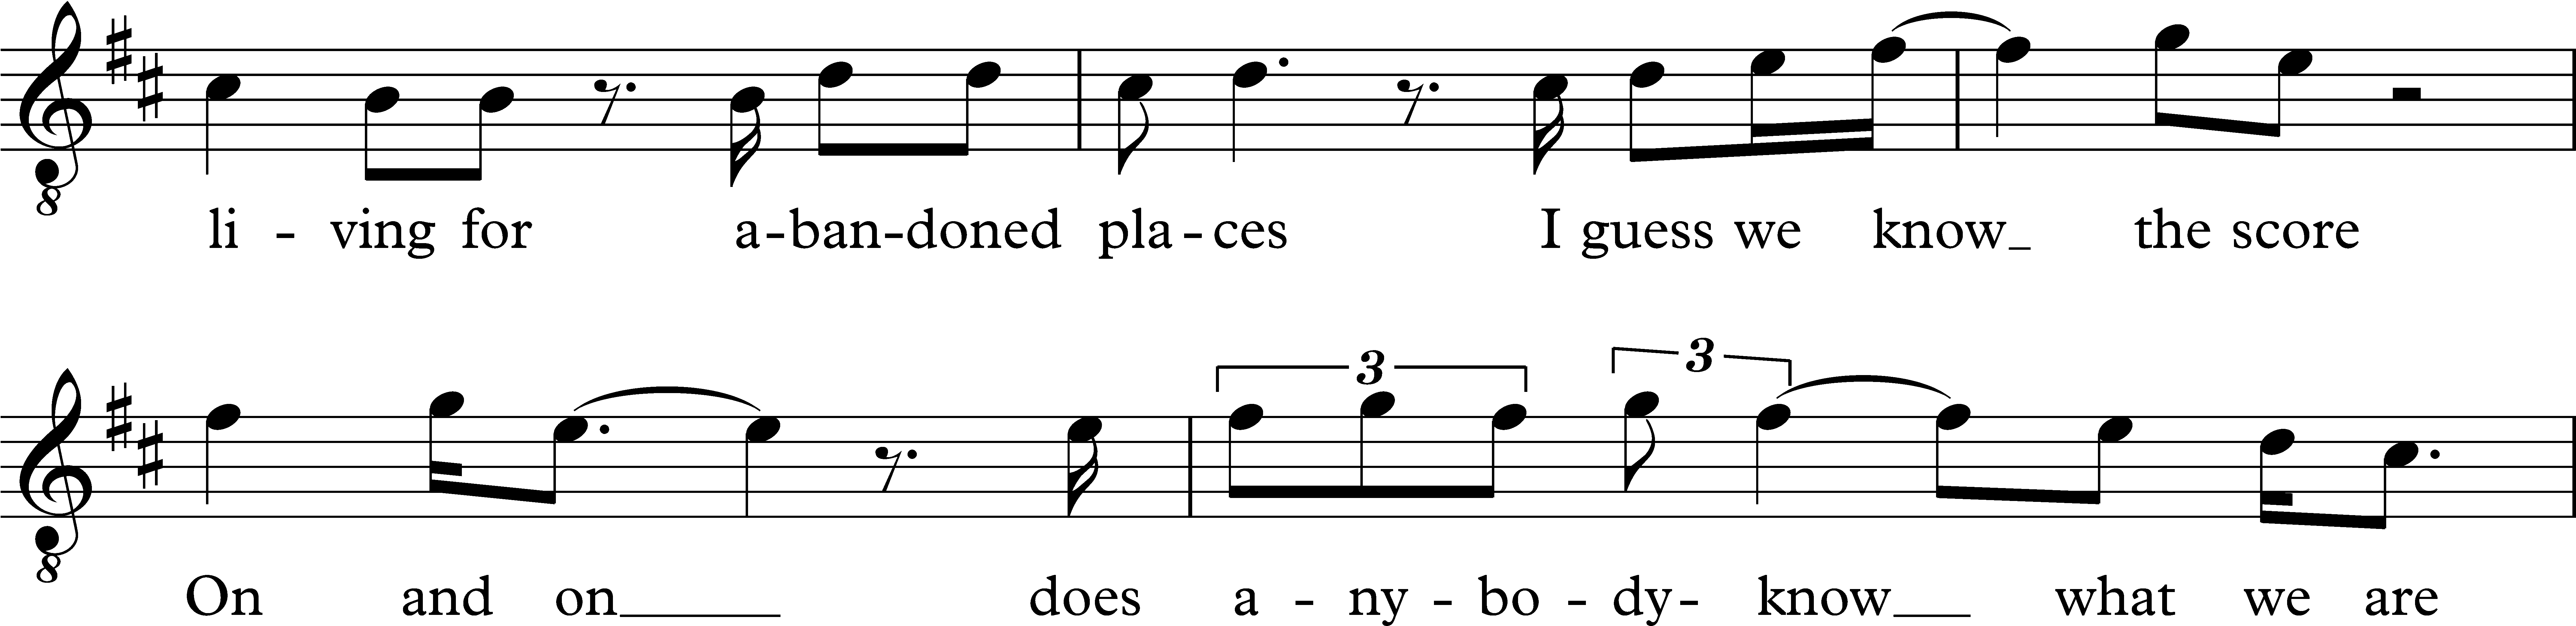
\includegraphics[width=\textwidth,keepaspectratio]{vox/voice1}
 \caption{Voce al minuto \(0:26\)}
 \label{fig:voice1}
\end{figure}

Da queste prime battute possiamo osservare anche un altro dettaglio importante circa la registrazione della traccia: se infatti ascoltiamo con attenzione la traccia isolata della voce (aiutandoci magari con un po' di compressione) e andiamo a \(0:22\), possiamo sentire come il respiro che segue a \emph{"empty spaces"} sia tagliato. Questo smentisce la famosa leggenda che Freddie abbia registrato il pezzo in una sola take dopo quel magico bicchierino di vodka, ma naturalmente non rende in alcun modo la tecnica del cantante meno pulita; il montaggio di numerose take per costruire la traccia finale per il disco, infatti, è una tecnica di produzione diffusa fin dai tempi dei Beatles, e i \emph{Queen} se n'erano serviti fin dagli inizi (per confronto, si ascolti quel \emph{"carry on"} che occorre al minuto \(1:39\) di Bohemian Rhapsody).

\begin{wrapfigure}{L}{0.35\textwidth}
 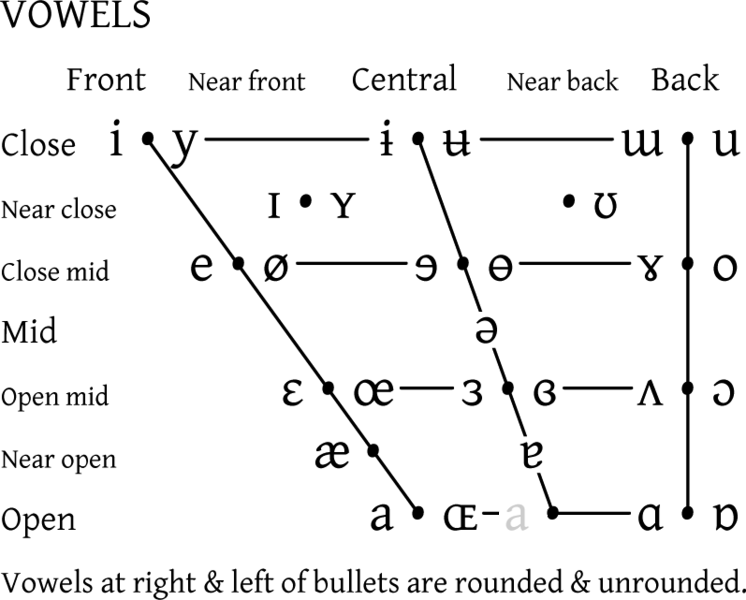
\includegraphics[width=\linewidth]{vox/vowels}
 \caption{Trapezio vocalico}
 \label{fig:vowels}
 \hspace{1cm}
 \centering
\end{wrapfigure}

Meritevole di attenzione è anche il segmento \emph{"Hold the line"} (\(0:52\)): quel LA\(_{4}\), oltre a essere una nota discretamente alta, è infatti presa con una vocale chiusa (quel \textipa{/U/} della figura~\ref{fig:vowels}, vocale molto comune soprattutto nell'inglese britannico), e le vocali di questo tipo tendono a indurre un passaggio alla voce di testa, dal momento che comportano un innalzamento del palato nel momento in cui vengono articolate. Questo passaggio non è necessariamente da evitare, anzi: riprendendo come esempio Bohemian Rhapsody, possiamo individuare quel tipo di passaggio al minuto \(2:29\), nella coda di quel \emph{"Mama, ooh"}, e in questo contesto risulta molto efficace. Ma la capacità di riuscire ad evitare il passaggio, come fatto da Mercury in questo passaggio della strofa, è prova di una grande padronanza della propria vocalità.

Più avanti nella traccia si trovano numerosi esempi di note ancora più alte di quel LA\(_{4}\): per cantare la famosa frase del ritornello, Freddie raggiunge infatti un SI\(_{4}\) articolando molto chiaramente ogni sillaba, nonostante in questo intervallo vocale sia difficile rendere intellegibili le parole a causa della grande apertura che la bocca deve tenere per raggiungere le note. Non solo: durante lo special, infatti, raggiunge di nuovo lo stesso SI\(_{4}\), che riesce a legare per un breve sedicesimo a un RE\(_{5}\). Questa è la nota più alta nel pezzo, e Freddie la riesce a toccare in un altro momento nell'ultimo ritornello; con buona approssimazione, si può dire che la zona intorno al RE\(_{5}\) costituisca il limite superiore che un tenore può raggiungere, e negli anni '\(80\) Mercury preferiva evitare di toccare note così alte durante i live; quindi, il fatto che sia riuscito a raggiungerla in questa registrazione dimostra ancora una volta di cosa fosse capace questo straordinario artista.

\begin{figure}[H]
 \centering
 \begin{minipage}{0.4\textwidth}
  \centering
  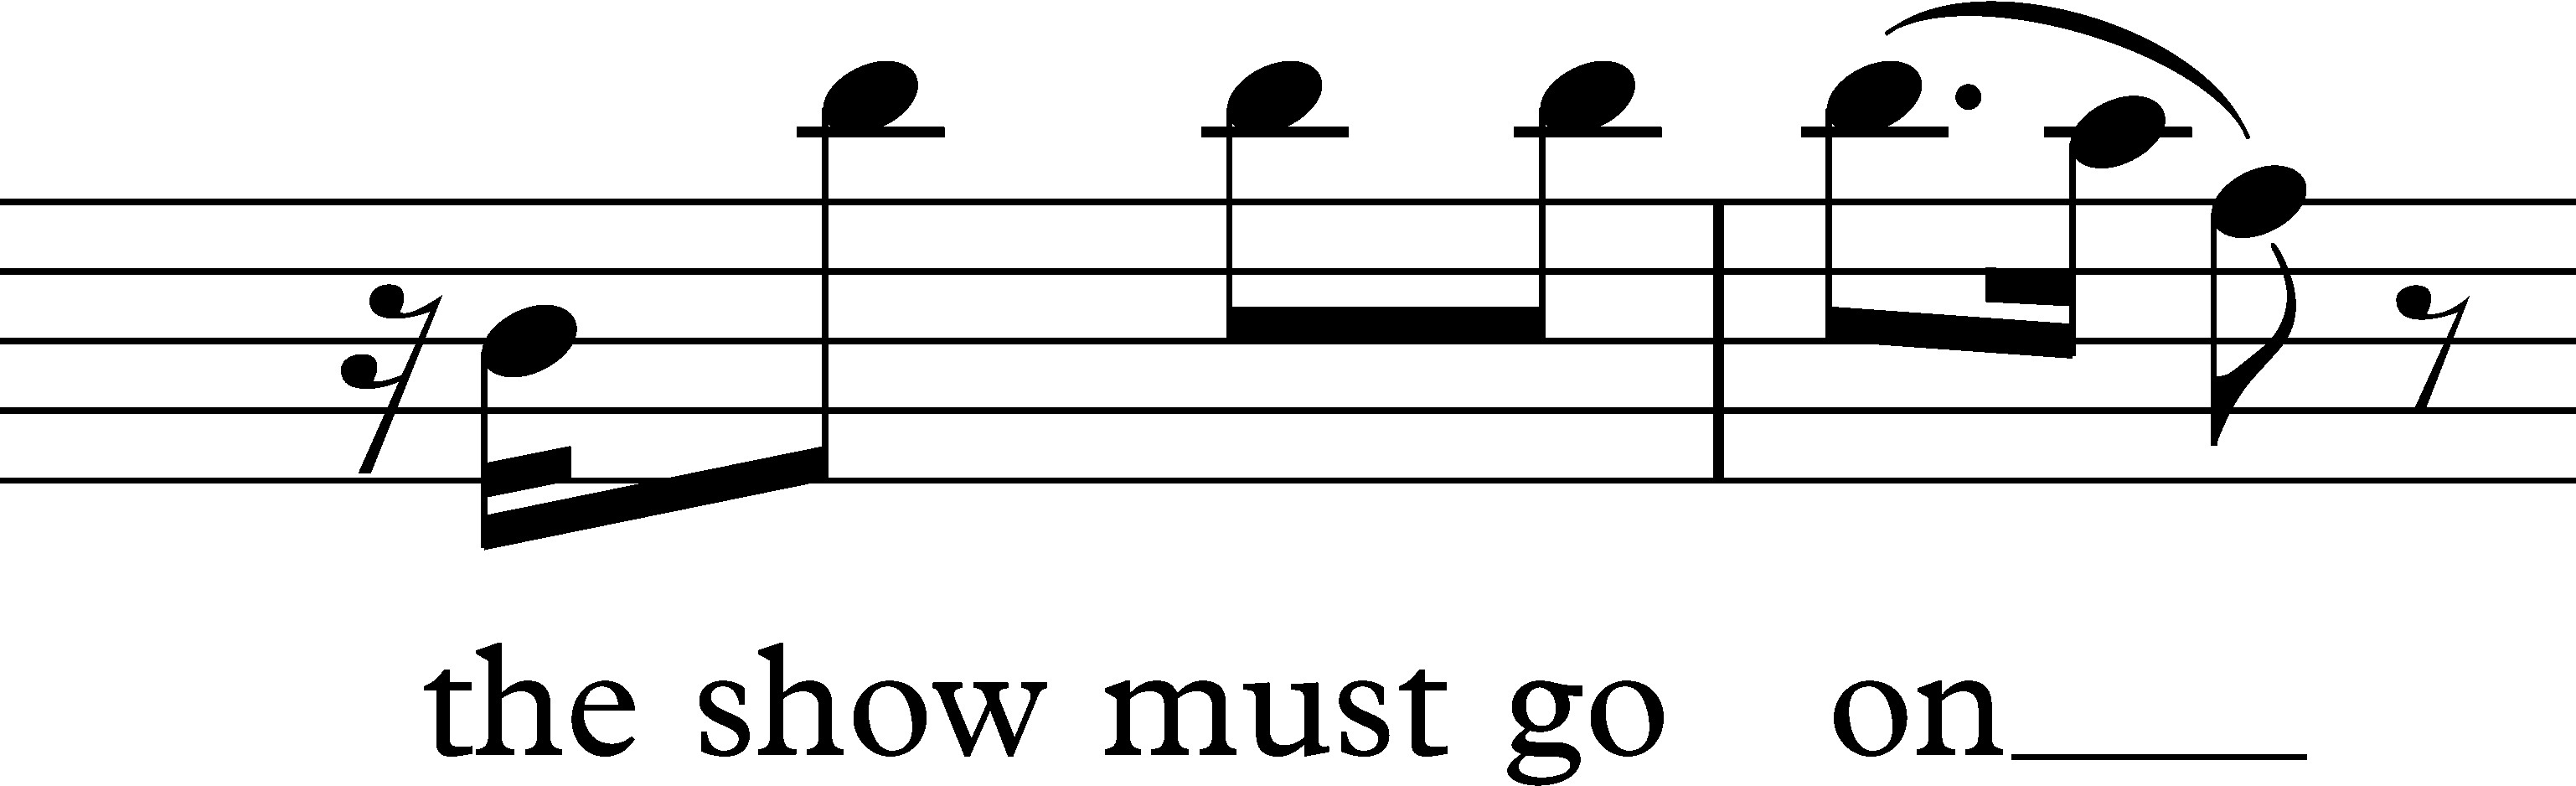
\includegraphics[width=\textwidth,keepaspectratio]{vox/voice2}
  \subcaption{Minuto \(0:59\)}
 \end{minipage}
 \hfill
 \begin{minipage}{0.4\textwidth}
  \centering
  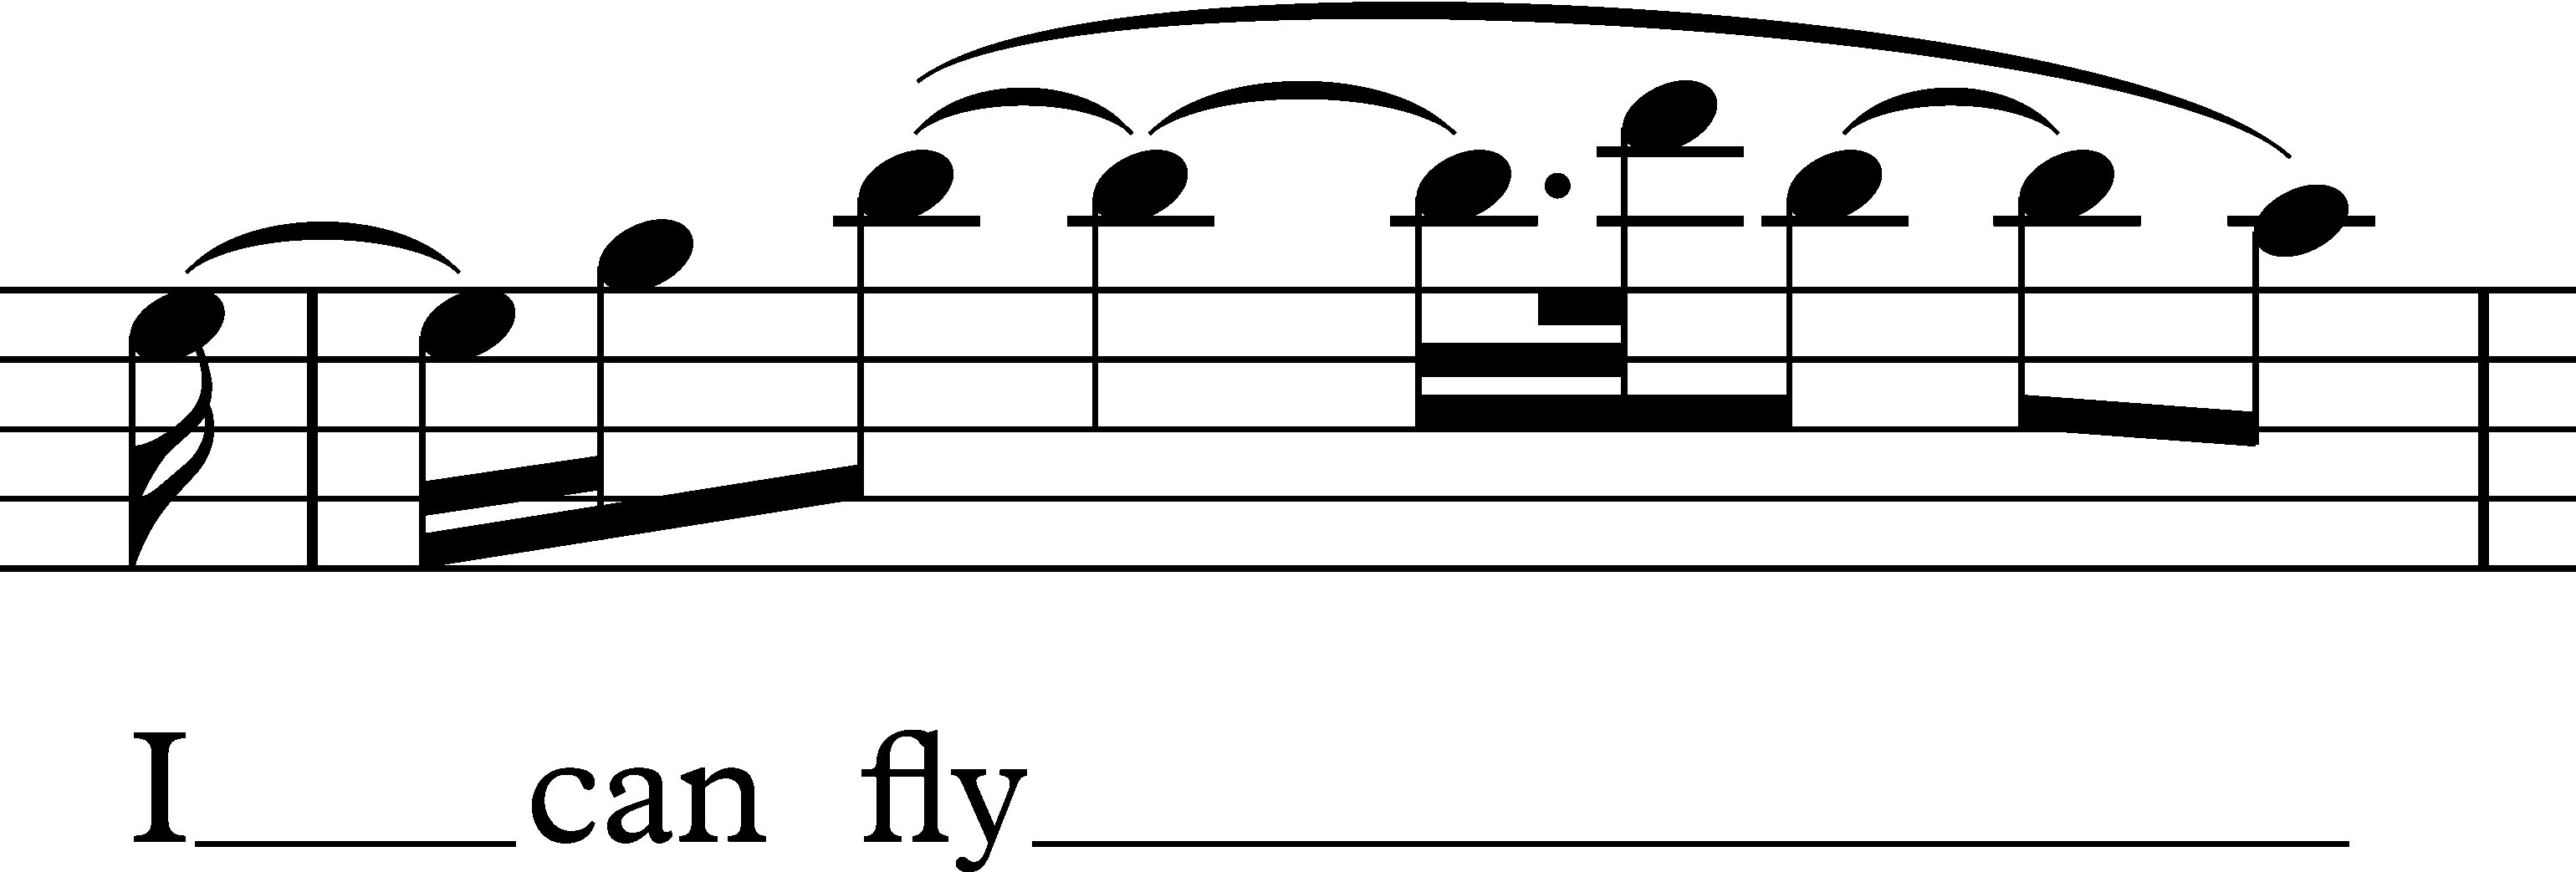
\includegraphics[width=\textwidth,keepaspectratio]{vox/voice3}
  \subcaption{Minuto \(3:00\)}
 \end{minipage}

 \begin{minipage}{0.4\textwidth}
  \centering
  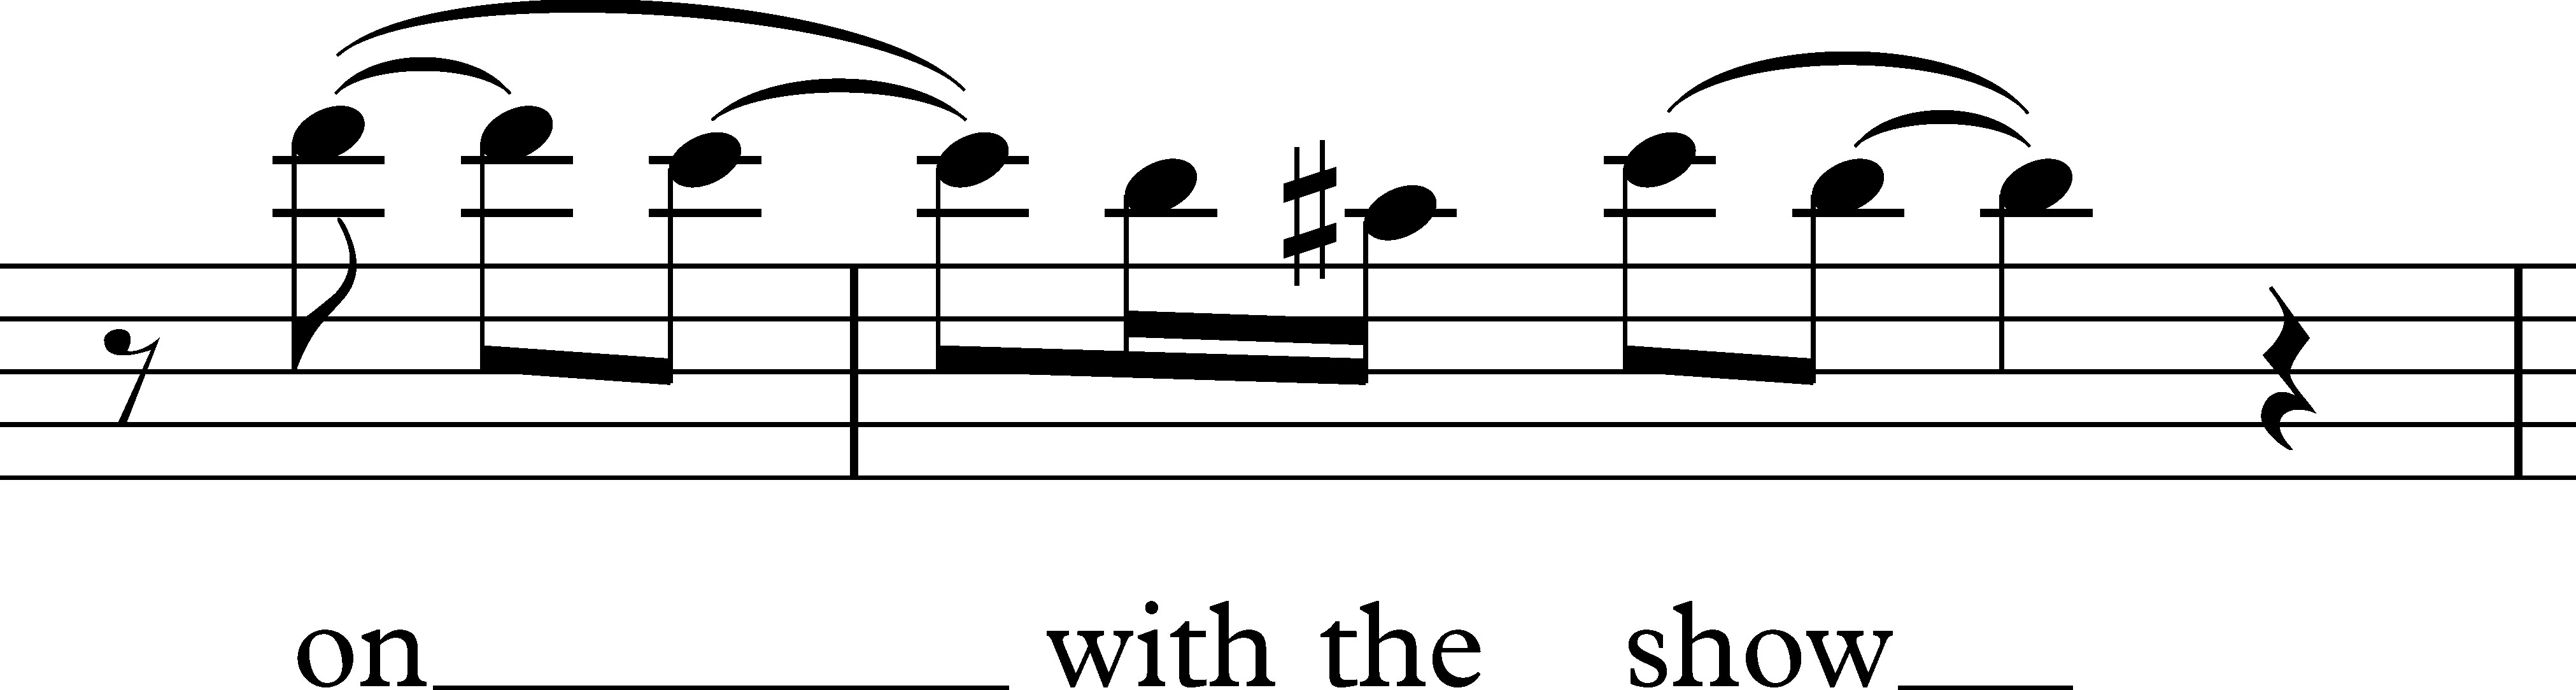
\includegraphics[width=\textwidth,keepaspectratio]{vox/voice4}
  \subcaption{Minuto \(2:22\)}
 \end{minipage}

 \caption{Esempi significativi delle note toccate da Mercury nel pezzo}
 \label{fig:guitSolo}
\end{figure}

\subsubsection{Seconde voci e cori}
Rispetto ad altri pezzi dei Queen, in questo i cori e le seconde voci hanno un ruolo molto ridotto; è plausibile ipotizzare che sia stato deciso così per lasciare che la voce solista di Mercury si prendesse tutto lo spazio di cui aveva bisogno.

I cori infatti non compaiono fino alla metà della seconda strofa, al minuto \(1:47\), dove vanno a ripetere le frasi della voce solista \emph{"I'm learning"} e \emph{"turning"}; ogni ripetizione viene posizionata, alternativamente, a sinistra e destra dell'immagine stereo, in modo da simulare un effetto di ping-pong delay, che ricorda un po' l'idea su cui Brian May aveva costruito la sezione centrale del brano \emph{The Prophet's Song}.

Quest'idea viene ripresa anche per l'ultimo ritornello, quello dopo lo special. In questo è presente una prima traccia di cori che, come nel secondo ritornello, armonizza la linea vocale con un accordo completo di Bm in secondo rivolto, mentre invece una seconda traccia le backing vocals (campionate da quelle della prima traccia) ripetono questa figura, e quella che presumibilmente è un'automazione di pan fa attraversare a questa traccia l'immagine stereo partendo dal canale sinistro.

\begin{figure}[H]
 \centering
 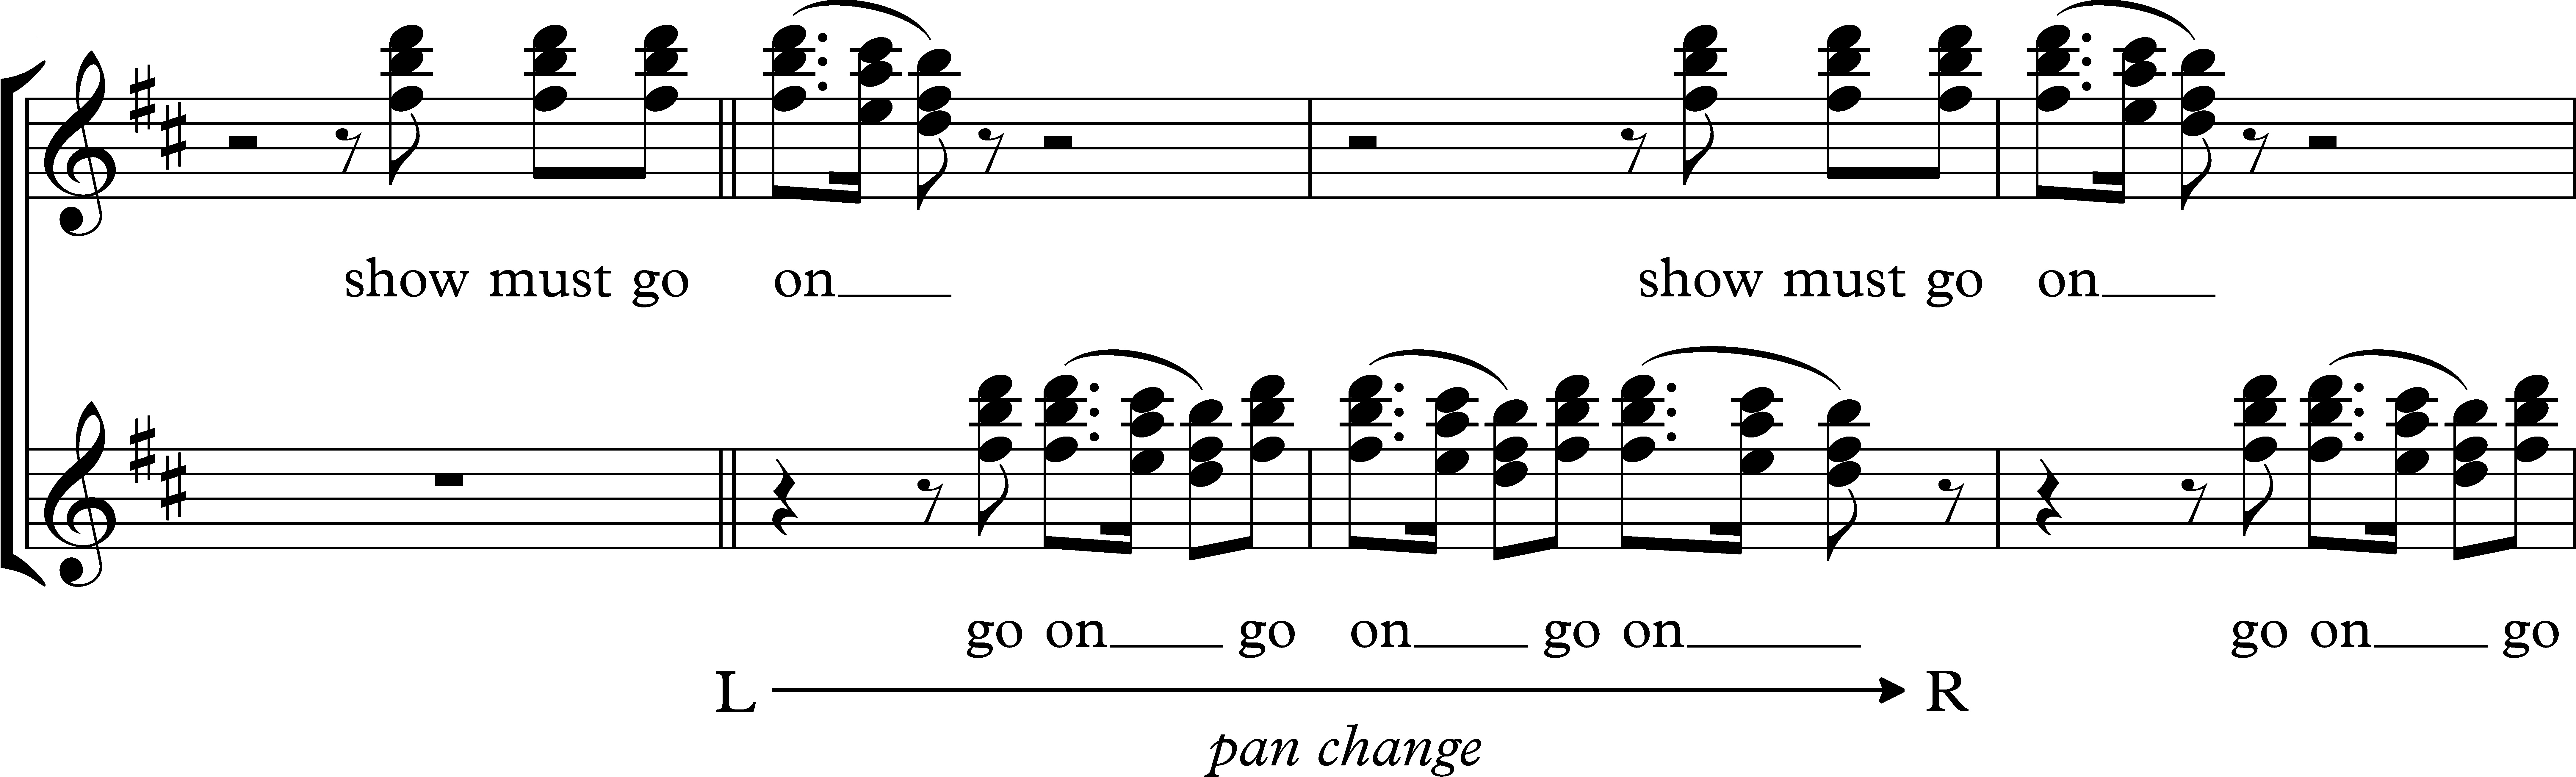
\includegraphics[width=\textwidth,keepaspectratio]{back_vox/choir1}
 \caption{Ultimo ritornello, minuto \(3:05\)}
 \label{fig:choir1}
\end{figure}

In modo simile viene anche costruita la coda del pezzo, eseguita solamente dai cori a cappella. La prima traccia esegue un accordo di Bm, inizialmente in secondo rivolto, successivamente in primo rivolto e infine in posizione fondamentale; i cambi tra questi sono raccordati da delle brevi istanze di A. Una seconda traccia, che di nuovo utilizza dei campionamenti della prima, ripete indefinitamente quel \emph{"go on"} nell'attesa che il fade out termini il pezzo (si veda lo spartito in figura~\ref{fig:choir2} per chiarimenti).

\begin{figure}[H]
 \centering
 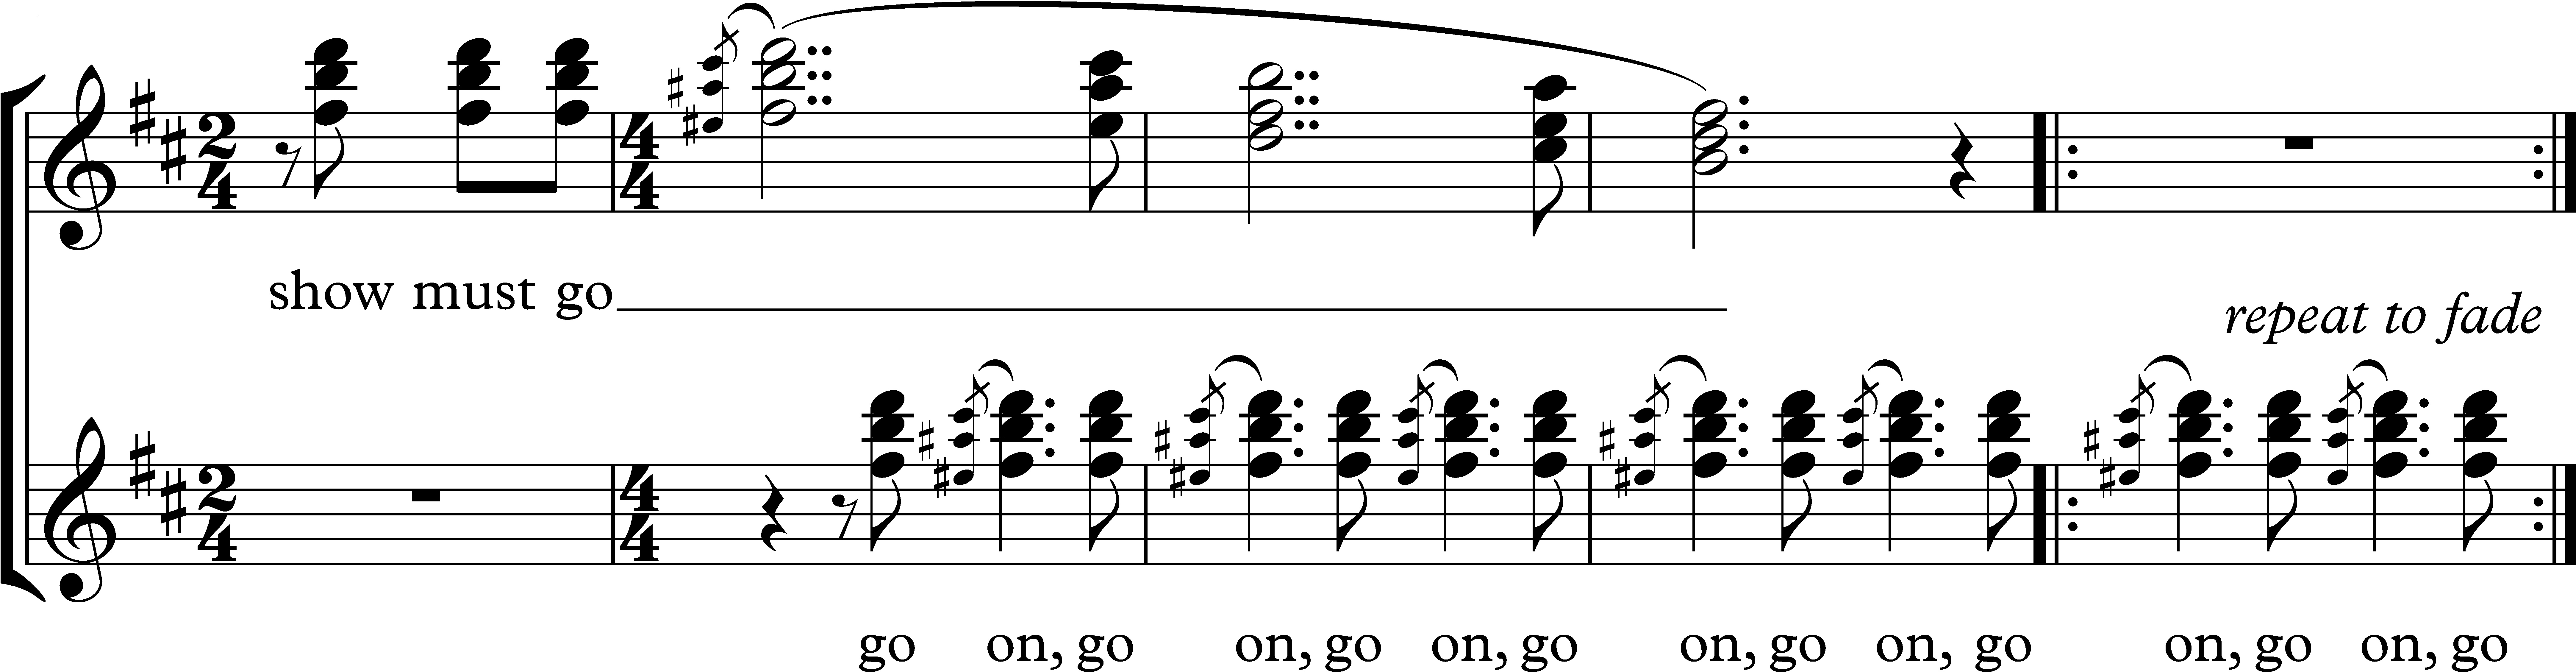
\includegraphics[width=\textwidth,keepaspectratio]{back_vox/choir2}
 \caption{Coda del brano, minuto \(3:52\)}
 \label{fig:choir2}
\end{figure}

\subsubsection{Tastiere}
Nel pezzo sono presenti due distinte tracce di tastiera, entrambe suonate dal chitarrista Brian May su un \emph{Korg M1}.

Nella prima traccia una patch che sembra un ensamble di archi esegue il tema in ottavi ribattuti costruito sul giro di accordi, che costituisce una solida ossatura su cui vengono disposti i restanti elementi del brano e in cui viene costruito il groove della batteria (figura~\ref{fig:key1}). L'idea di un giro costruito su degli ottavi ribattuti non si può certamente definire un tratto stilistico, ma nemmeno è un caso isolato nella discografia dei Queen. Molto spesso il gruppo è ricorso a uno stile di accompagnamento simile, soprattutto nel periodo degli anni '\(80\). Questo schema possiamo ritrovarlo, ad esempio, nell'introduzione della versione del singolo della celeberrima \emph{I Want to Break Free}, in cui viene suonato da un synth, oppure anche al minuto \(2:54\) di \emph{Hammer To Fall}.

\begin{figure}[H]
 \centering
 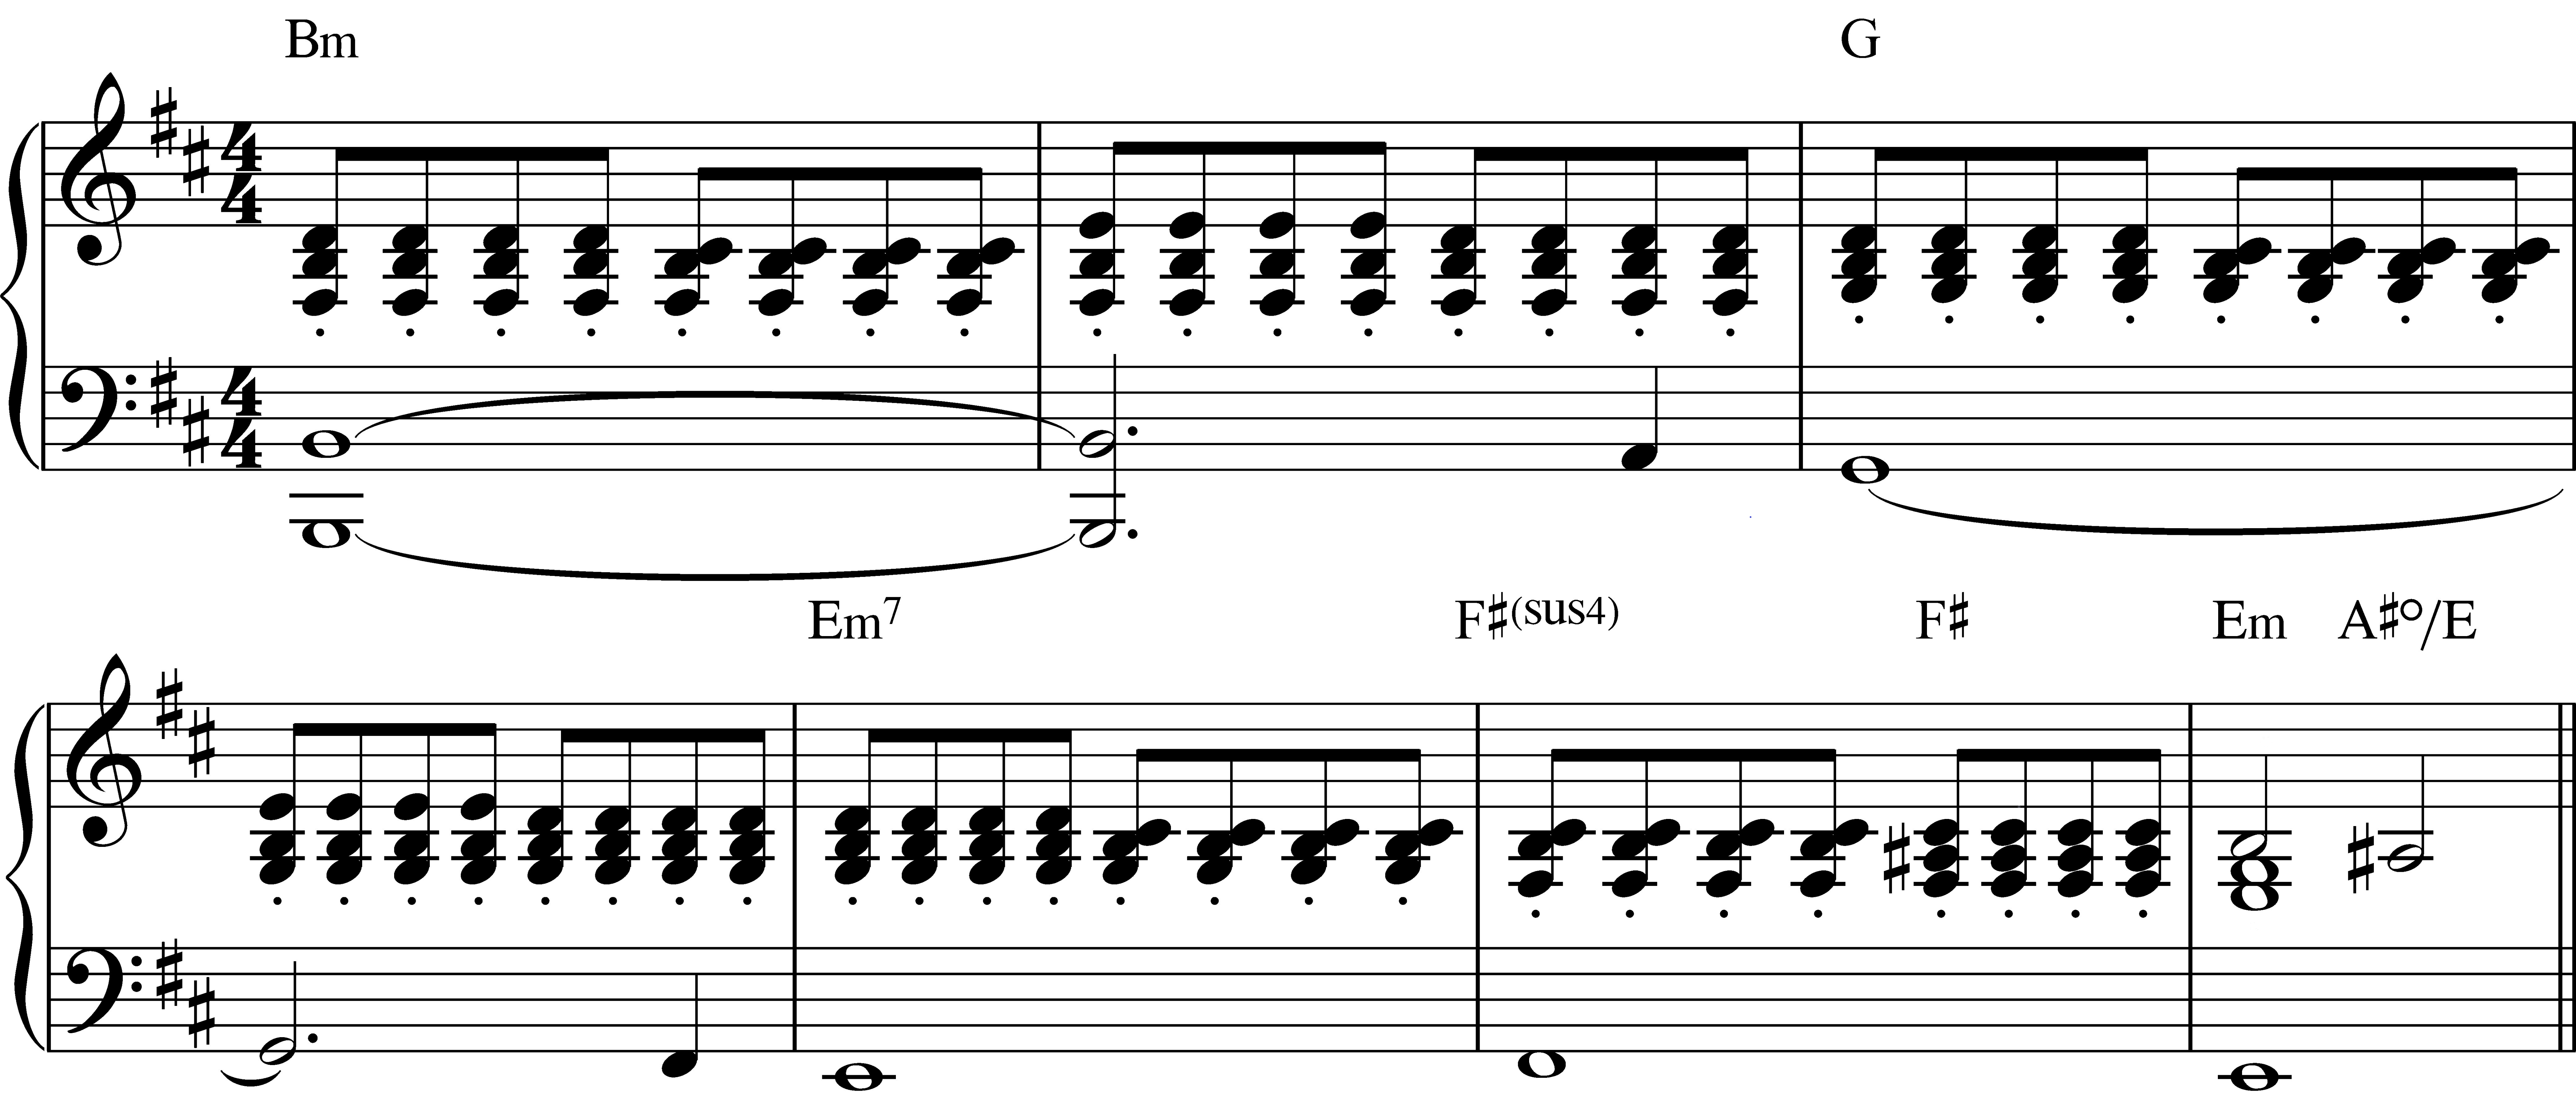
\includegraphics[width=\textwidth,keepaspectratio]{keys/key1}
 \caption{Intro completa del brano}
 \label{fig:key1}
\end{figure}

L'uso degli archi nelle ballate rock è diffuso fin dai tempi dei Beatles: si pensi ad esempio al quartetto d'archi che ha preso parte alla registrazione di \emph{Yesterday} assieme a Paul McCartney nel \(1965\), o addirittura a \emph{Eleanor Rigby}, la cui componente strumentale è costituita esclusivamente da una sezione di \(8\) archi. Un arrangiamento d'archi e una sezione che lo suonassero, però, rimasero a lungo appannaggio esclusivo di grandi produzioni; ma con l'uscita negli anni '\(70\) dei primi strumenti capaci di fornire campionamenti di fiati e archi di qualità soddisfacente (affermazione controversa, ma in questa sede non ci interessa approfondire l'argomento) a prezzi abbordabili, come il \emph{mellotron}, molti più gruppi riuscirono ad inserire suoni orchestrali nei pezzi. Ne sono esempio l'intro della celeberrima \emph{Stairway to Heaven}, che presenta una linea di flauto suonata da John Paul Jones su un mellotron, l'intro di \emph{Watcher of the Skies} dei Genesis, oppure ancora \emph{Dream On} degli Aerosmith. Con l'introduzione delle prime workstation negli anni '\(80\), ancora più economiche e versatili e, soprattutto, in linea con le sonorità tipiche dell'epoca, l'uso degli archi nela musica pop e rock si diffuse ulteriormente, nonostante la qualità timbrica fosse sensibilmente inferiore anche rispetto al mellotron; lo stesso Brian May, durante il Live Aid, suonò \emph{Who Wants to Live Forever} su una Yamaha DX7.

La seconda traccia invece è un pad di archi, più morbido del suono della traccia principale, e funge sostanzialmente da rinforzo al muro sonoro. Durante le strofe e i ritornelli infatti in questa traccia non vengono suonati bassi, che avrebbero rischiato di intasare la zona delle frequenze medio-basse, e non vengono nemmeno ribattuti gli ottavi; viene semplicemente cambiata la voce dell'accordo, in modo da seguire il tema principale.\\
Durante lo special questo pad si muove un'ottava sopra rispetto alla tastiera principale, in modo da irrobustire lo spessore del suono per avvicinarsi quanto più possibile alla potenza generata da una vera sezione orchestrale.

\subsubsection{Chitarre}
Le tracce di chitarra sono ancora due: una esegue principalmente le parte soliste, quindi i soli ed alcuni fills, e la seconda esegue un accompagnamento.

La chitarra entra nel pezzo al minuto \(0:34\) suonando un MI con la tecnica del volume swell: questa consiste nel plettrare una corda tenendo il potenziometro del volume (o alternativamente un pedale volume) a \(0\) e aumentarlo gradualmente fino a raggiungere il valore massimo, in modo da ridurre l'attacco e rendere l'articolazione simile a quella di uno strumento ad arco suonato con archetto; esempi di questa tecnica si possono ritrovare anche nei Beatles (\emph{I Need You}, \emph{Yes It Is}, \emph{Wait}), anche se è più probabile che May l'abbia mutuata da Steve Hackett, avendola utilizzata anch'esso a più riprese.

Per quanto riguarda l'accompagnamento delle strofe, May sceglie di suonare bicordi di prima e quinta (schema che nell musica rock è colloquialmente noto come powerchord), smorzandone il sustain con il palm muting. Nonostante questa scelta sia molto semplice e non sia certo considerabile un tratto caratteristico, risulta molto funzionale al pezzo, in quanto accentua l'atmosfera solenne evocata dal pattern ritmico in ottavi del synth principale.

Nei ritornelli invece May abbandona la cadenza a ottavi suona accordi completi a \(3\) o \(4\) voci, più larghi; l'uso di accordi completi con la distorsione è un retaggio del rock degli anni '\(70\) e se ne possono trovare esempi nei Beatles, Led Zeppelin e in quasi tutti i gruppi dell'epoca, oltre che negli stessi Queen (in figura~\ref{fig:mother} Tie Your Mother Down, pezzo dal disco \emph{A Day At the Races} del \(1976\)). Per ingrossare ulteriormente il suono, aggiunge alla distorsione della chitarra un effetto phaser/flanger, molto in voga nelle produzioni hard rock anni '\(80\).

\begin{figure}[H]
 \centering
 
\includegraphics[width=\textwidth,keepaspectratio]{guitars/mother}
 \caption{Riff principale di Tie Your Mother Down, si osservi in particolare la quarta battuta}
 \label{fig:mother}
\end{figure}

Nello special, invece, May riduce la distorsione e accompagna con degli arpeggi (figura~\ref{fig:guitArp}); anche questa è un'idea ricorrente nelle parti di chitarra dei Queen, si veda ad esempio il riff principale di \emph{Under Pressure} (figura~\ref{fig:guitPres}).

\begin{figure}[H]
 \centering
 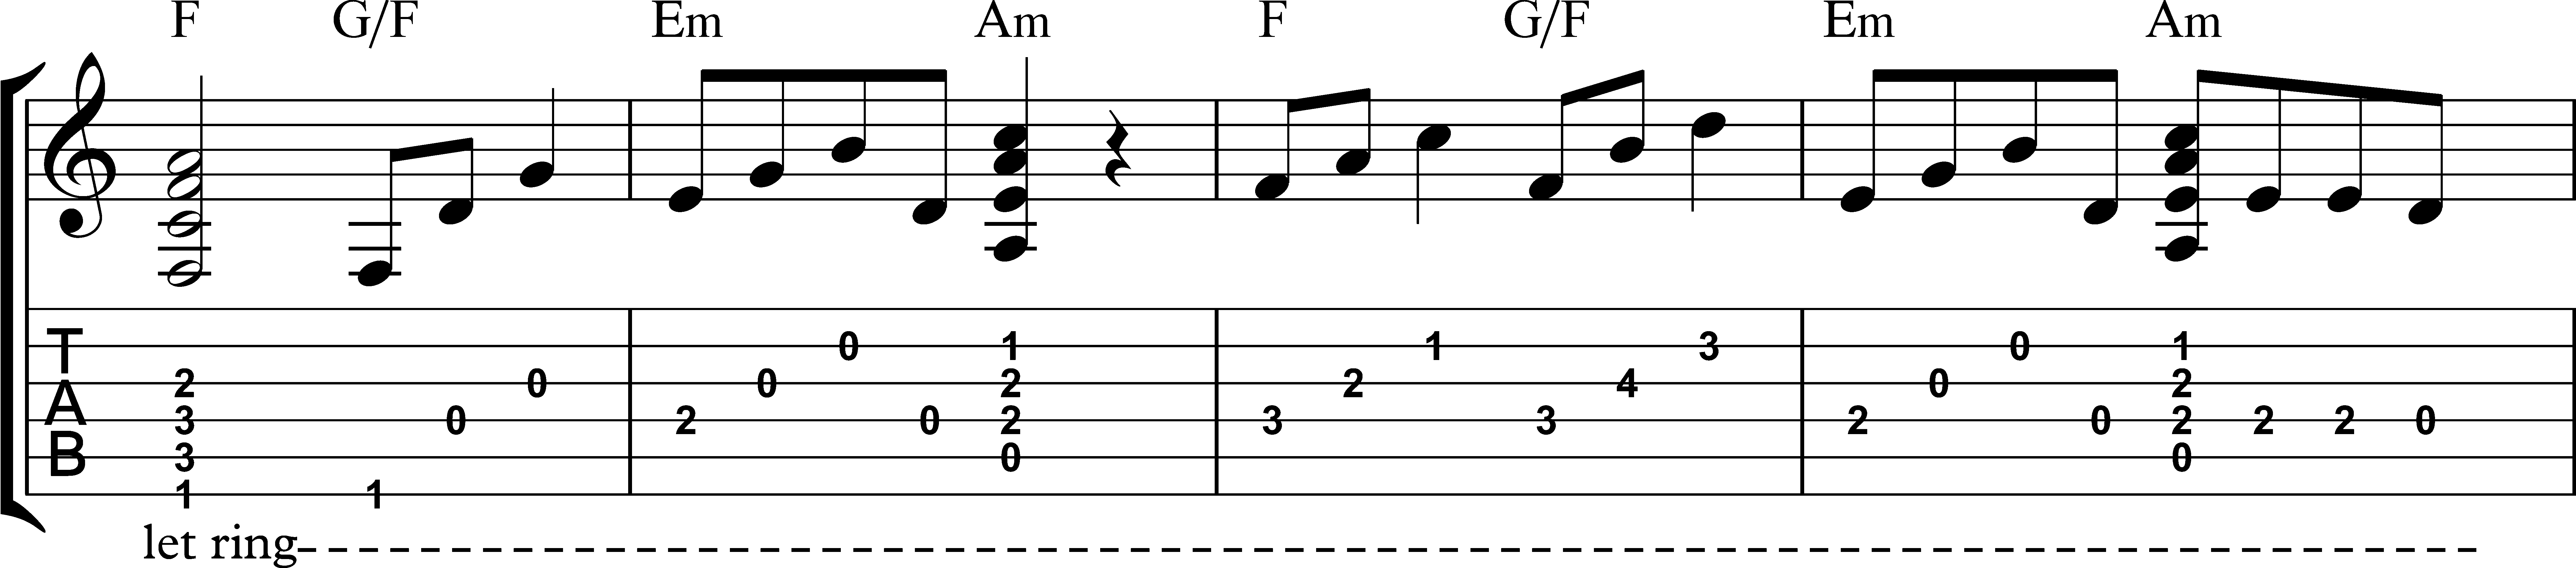
\includegraphics[width=\textwidth,keepaspectratio]{guitars/guit1}
 \caption{Chitarra, dal minuto \(2:48\)}
 \label{fig:guitArp}
\end{figure}

\begin{figure}[H]
 \centering
 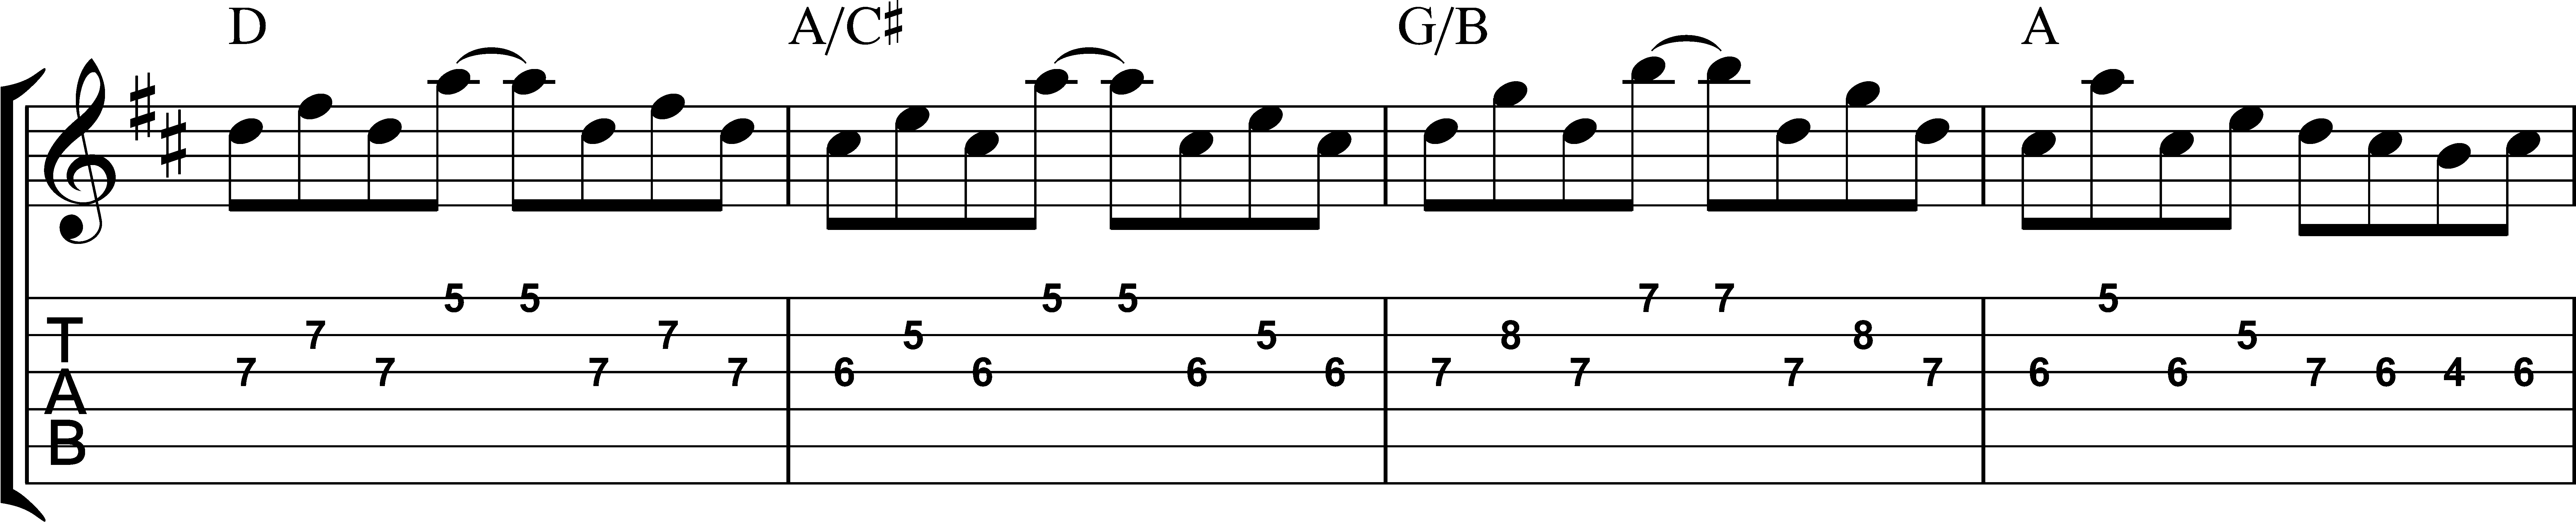
\includegraphics[width=\textwidth,keepaspectratio]{guitars/pressure}
 \caption{Riff di chitarra di Under Pressure}
 \label{fig:guitPres}
\end{figure}

Nonostante in questo pezzo ci siano solamente un paio di parti soliste molto brevi (minuti \(2:29\) e \(3:25\)) si può comunque riconoscere alcuni tratti distintivi dello stile di Brian May, come ad esempio la ripresa della linea vocale come incipit del secondo solo o l'uso di gruppi irregolari nelle parti più virtuosistiche (figura~\ref{fig:guitSolo}).

\begin{figure}[H]
 % \centering
 % \begin{minipage}{0.4\textwidth}
 %  \centering
 %  \includegraphics[width=\textwidth,keepaspectratio]{guitars/guit2}
 % 	 \subcaption{Minuto \(2:31\)}
 % \end{minipage}
 % \hfill
 \begin{minipage}{0.4\textwidth}
  \centering
  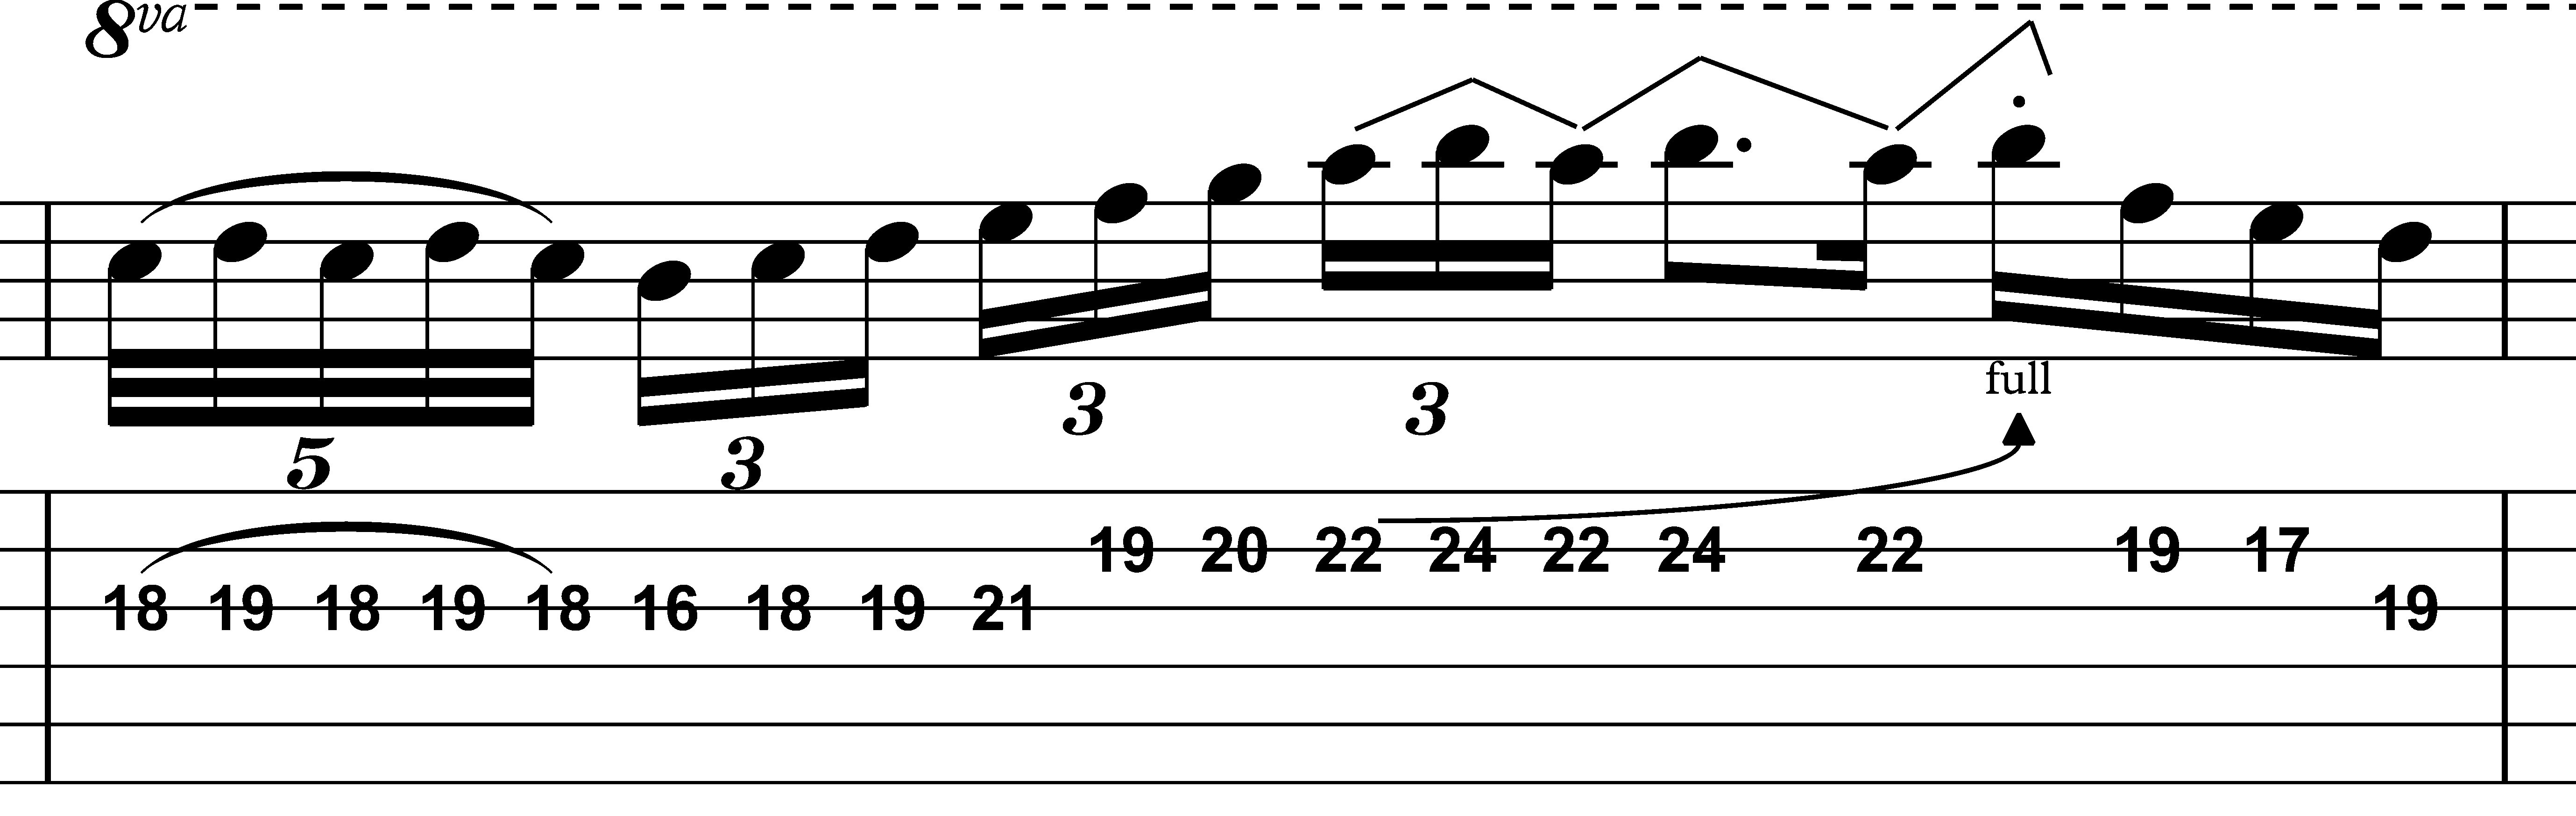
\includegraphics[width=\textwidth,keepaspectratio]{guitars/guit3_2}
  \subcaption{The Show Must Go On, minuto \(3:29\)}
 \end{minipage}
 \hfill
 \begin{minipage}{0.4\textwidth}
  \centering
  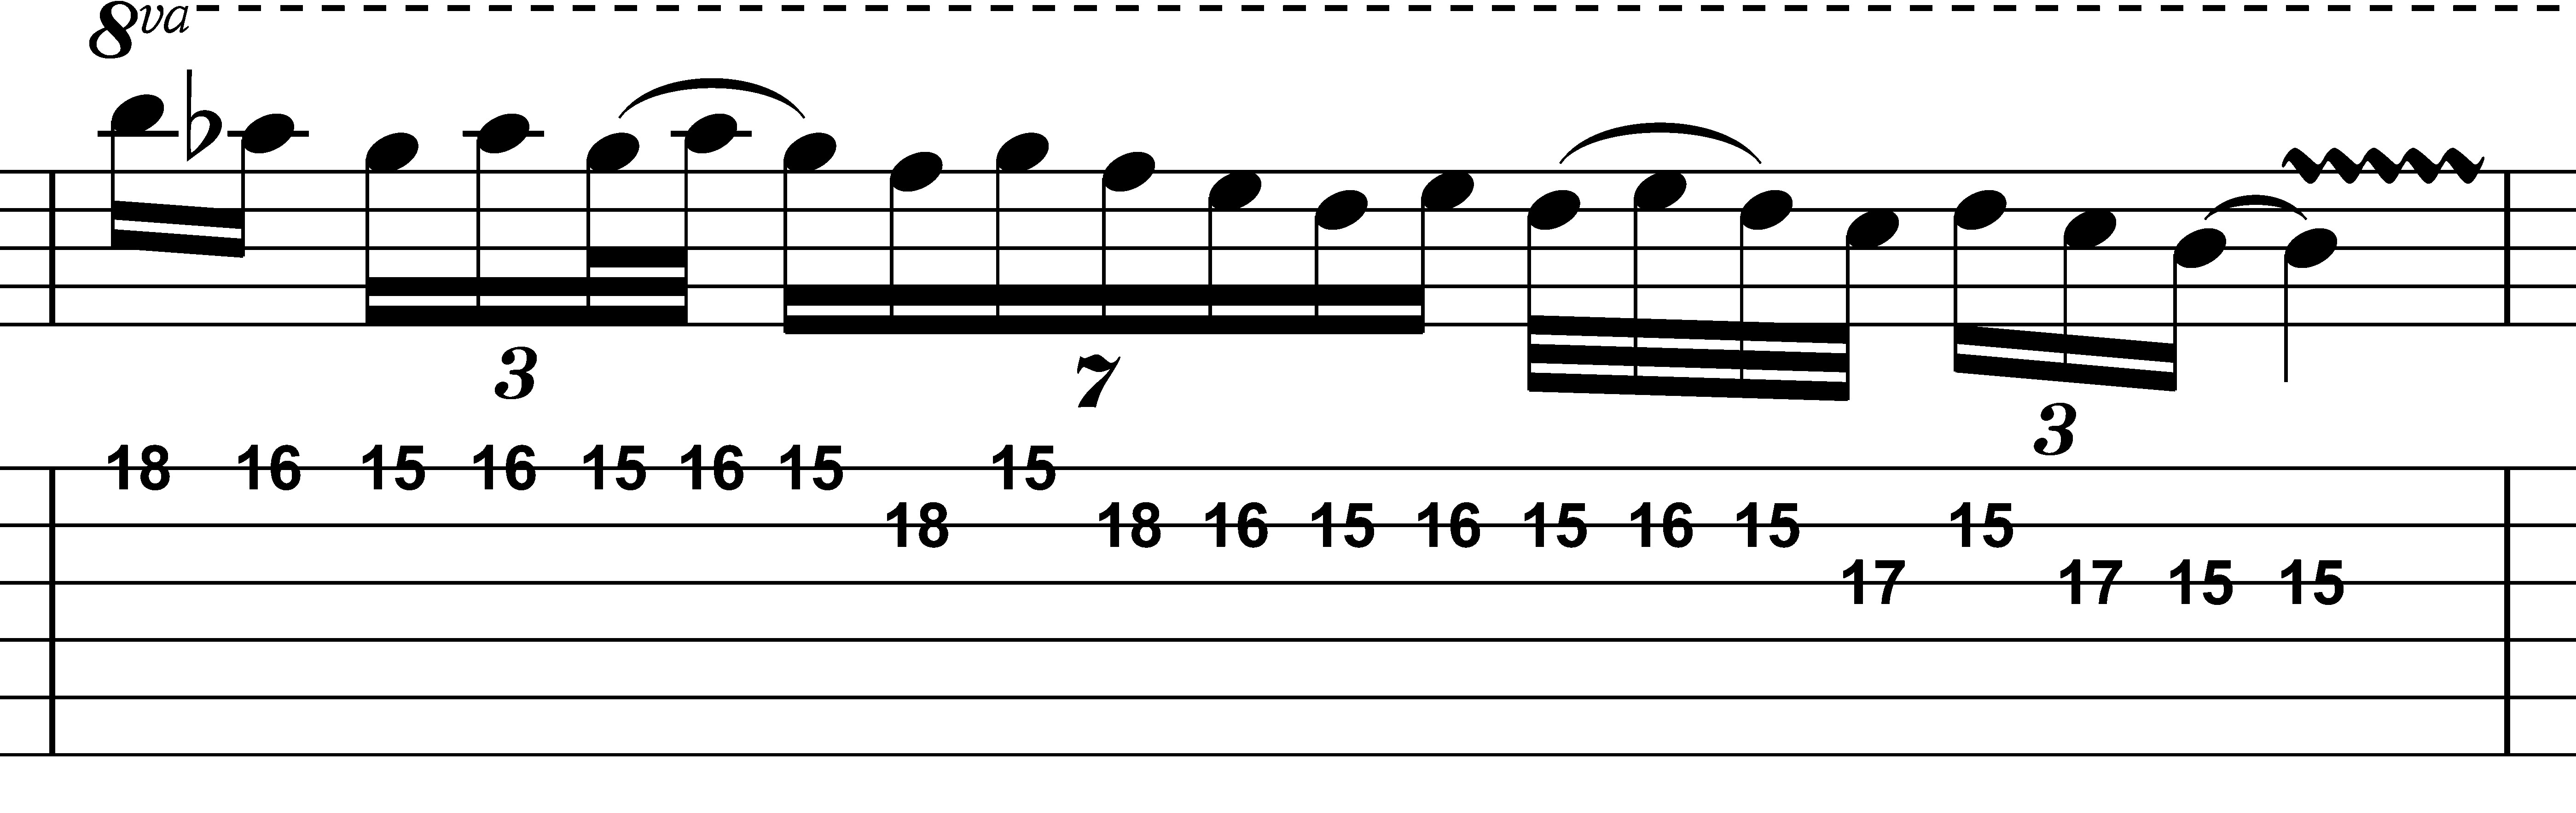
\includegraphics[width=\textwidth,keepaspectratio]{guitars/rhap}
  \subcaption{Bohemian Rhapsody, minuto \(2:47\)}
 \end{minipage}

 \caption{Alcuni esempi di uso di gruppi irregolari nei soli}
 \label{fig:guitSolo}
\end{figure}

Molto interessante anche la chiusura del primo solo, che presenta una linea discendente suonata con una tecnica per sporcare i bending ancora ripresa dagli anni '\(70\): May infatti plettra una nota sulla prima corda e un'altra, un tono più bassa, sulla seconda corda, e successivamente esegue un bending su quest'ultima per portarla alla stessa altezza di quella sulla prima corda. Questo naturalmente produce una piacevole "sporcatura" iniziale della nota, ma ha anche un secondo effetto: dal momento che, per quanto preciso possa essere un chitarrista, le due note non saranno mai del tutto equivalenti in termini di frequenza, ma questa differenza di pochi centesimi di tono contribuisce a rendere il suono molto più spesso; una tecnica simile si usa anche nei sintetizzatori quando si vanno ad accendere due o più oscillatori, ciascuno con un leggermente diverso valore di detune (figura~\ref{fig:bendSolo}).

\begin{figure}[H]
 \centering
 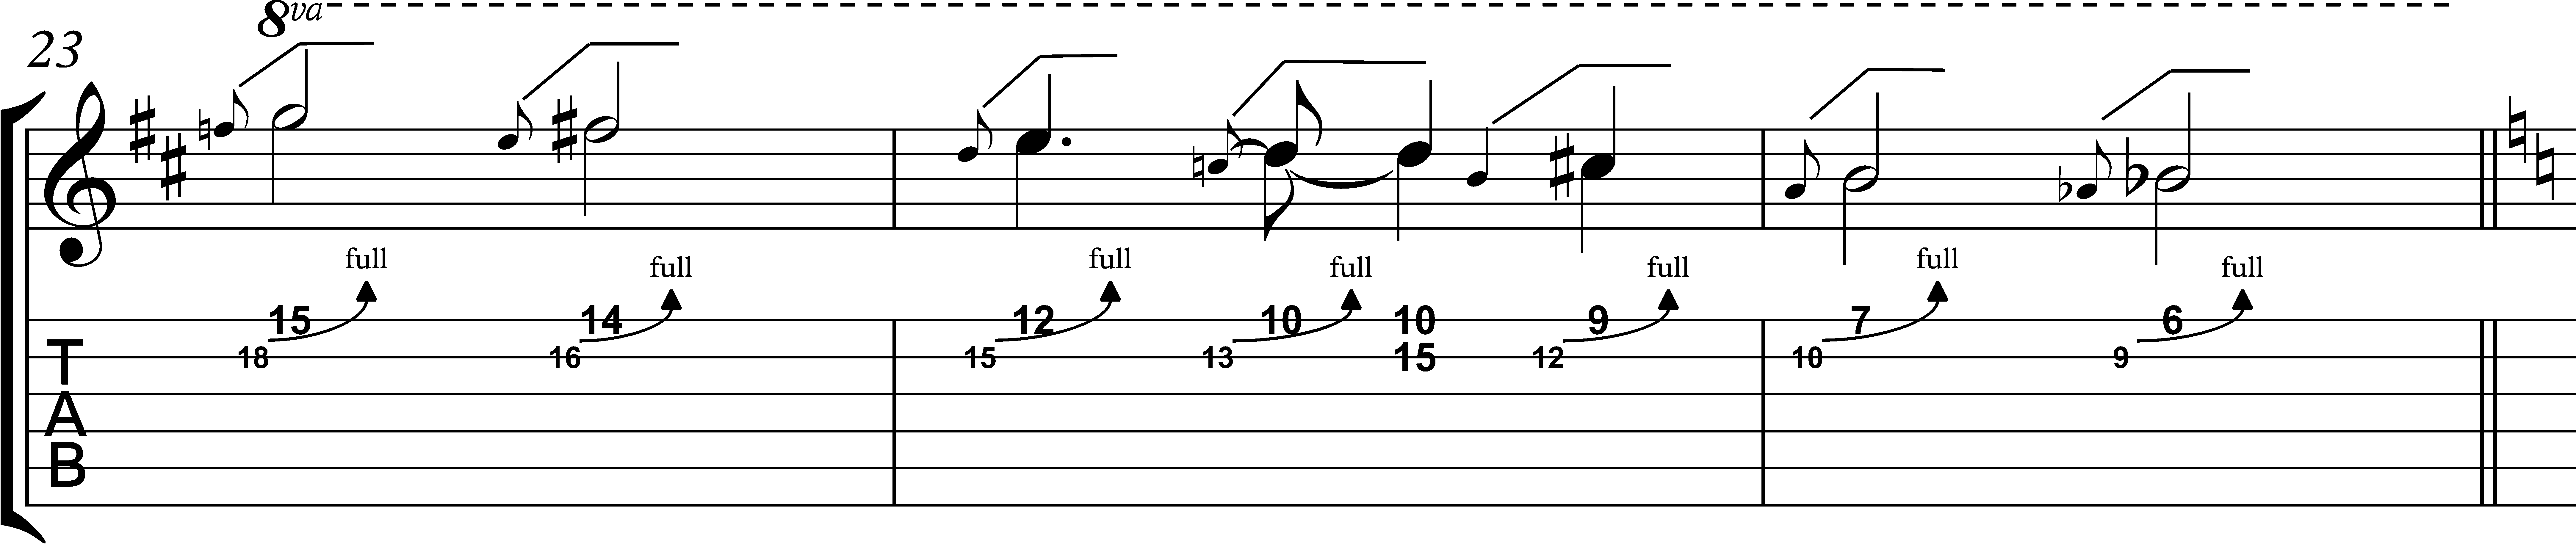
\includegraphics[width=\textwidth,keepaspectratio]{guitars/guit5}
 \caption{La sezione coi bend all'unisono, minuto \(2:40\)}
 \label{fig:bendSolo}
\end{figure}

In ultimo, non possiamo non notare come l'ultimo solo presenti uno dei tratti stilistici più riconoscibili degli arrangiamenti di chitarra di Brian May, ossia l'uso di numerose sovraincisioni per creare effetti orchestrali. Nel lancio di questo solo, infatti, la chitarra solista riprende l'idea della linea vocale, suonando però dei Fa\(\sharp\) anziché dei SI e  prendendo ogni nota con un bending per renderne l'articolazione più viva e simile a quella della voce umana; dietro a questa sono registrate altre tre tracce di chitarra, che vanno ad armonizzare quella frase con un accordo di Bm in secondo rivolto, esattamente la stessa parte eseguita dai cori nei normali ritornelli.

\begin{figure}[H]
 \begin{minipage}{0.4\textwidth}
  \centering
  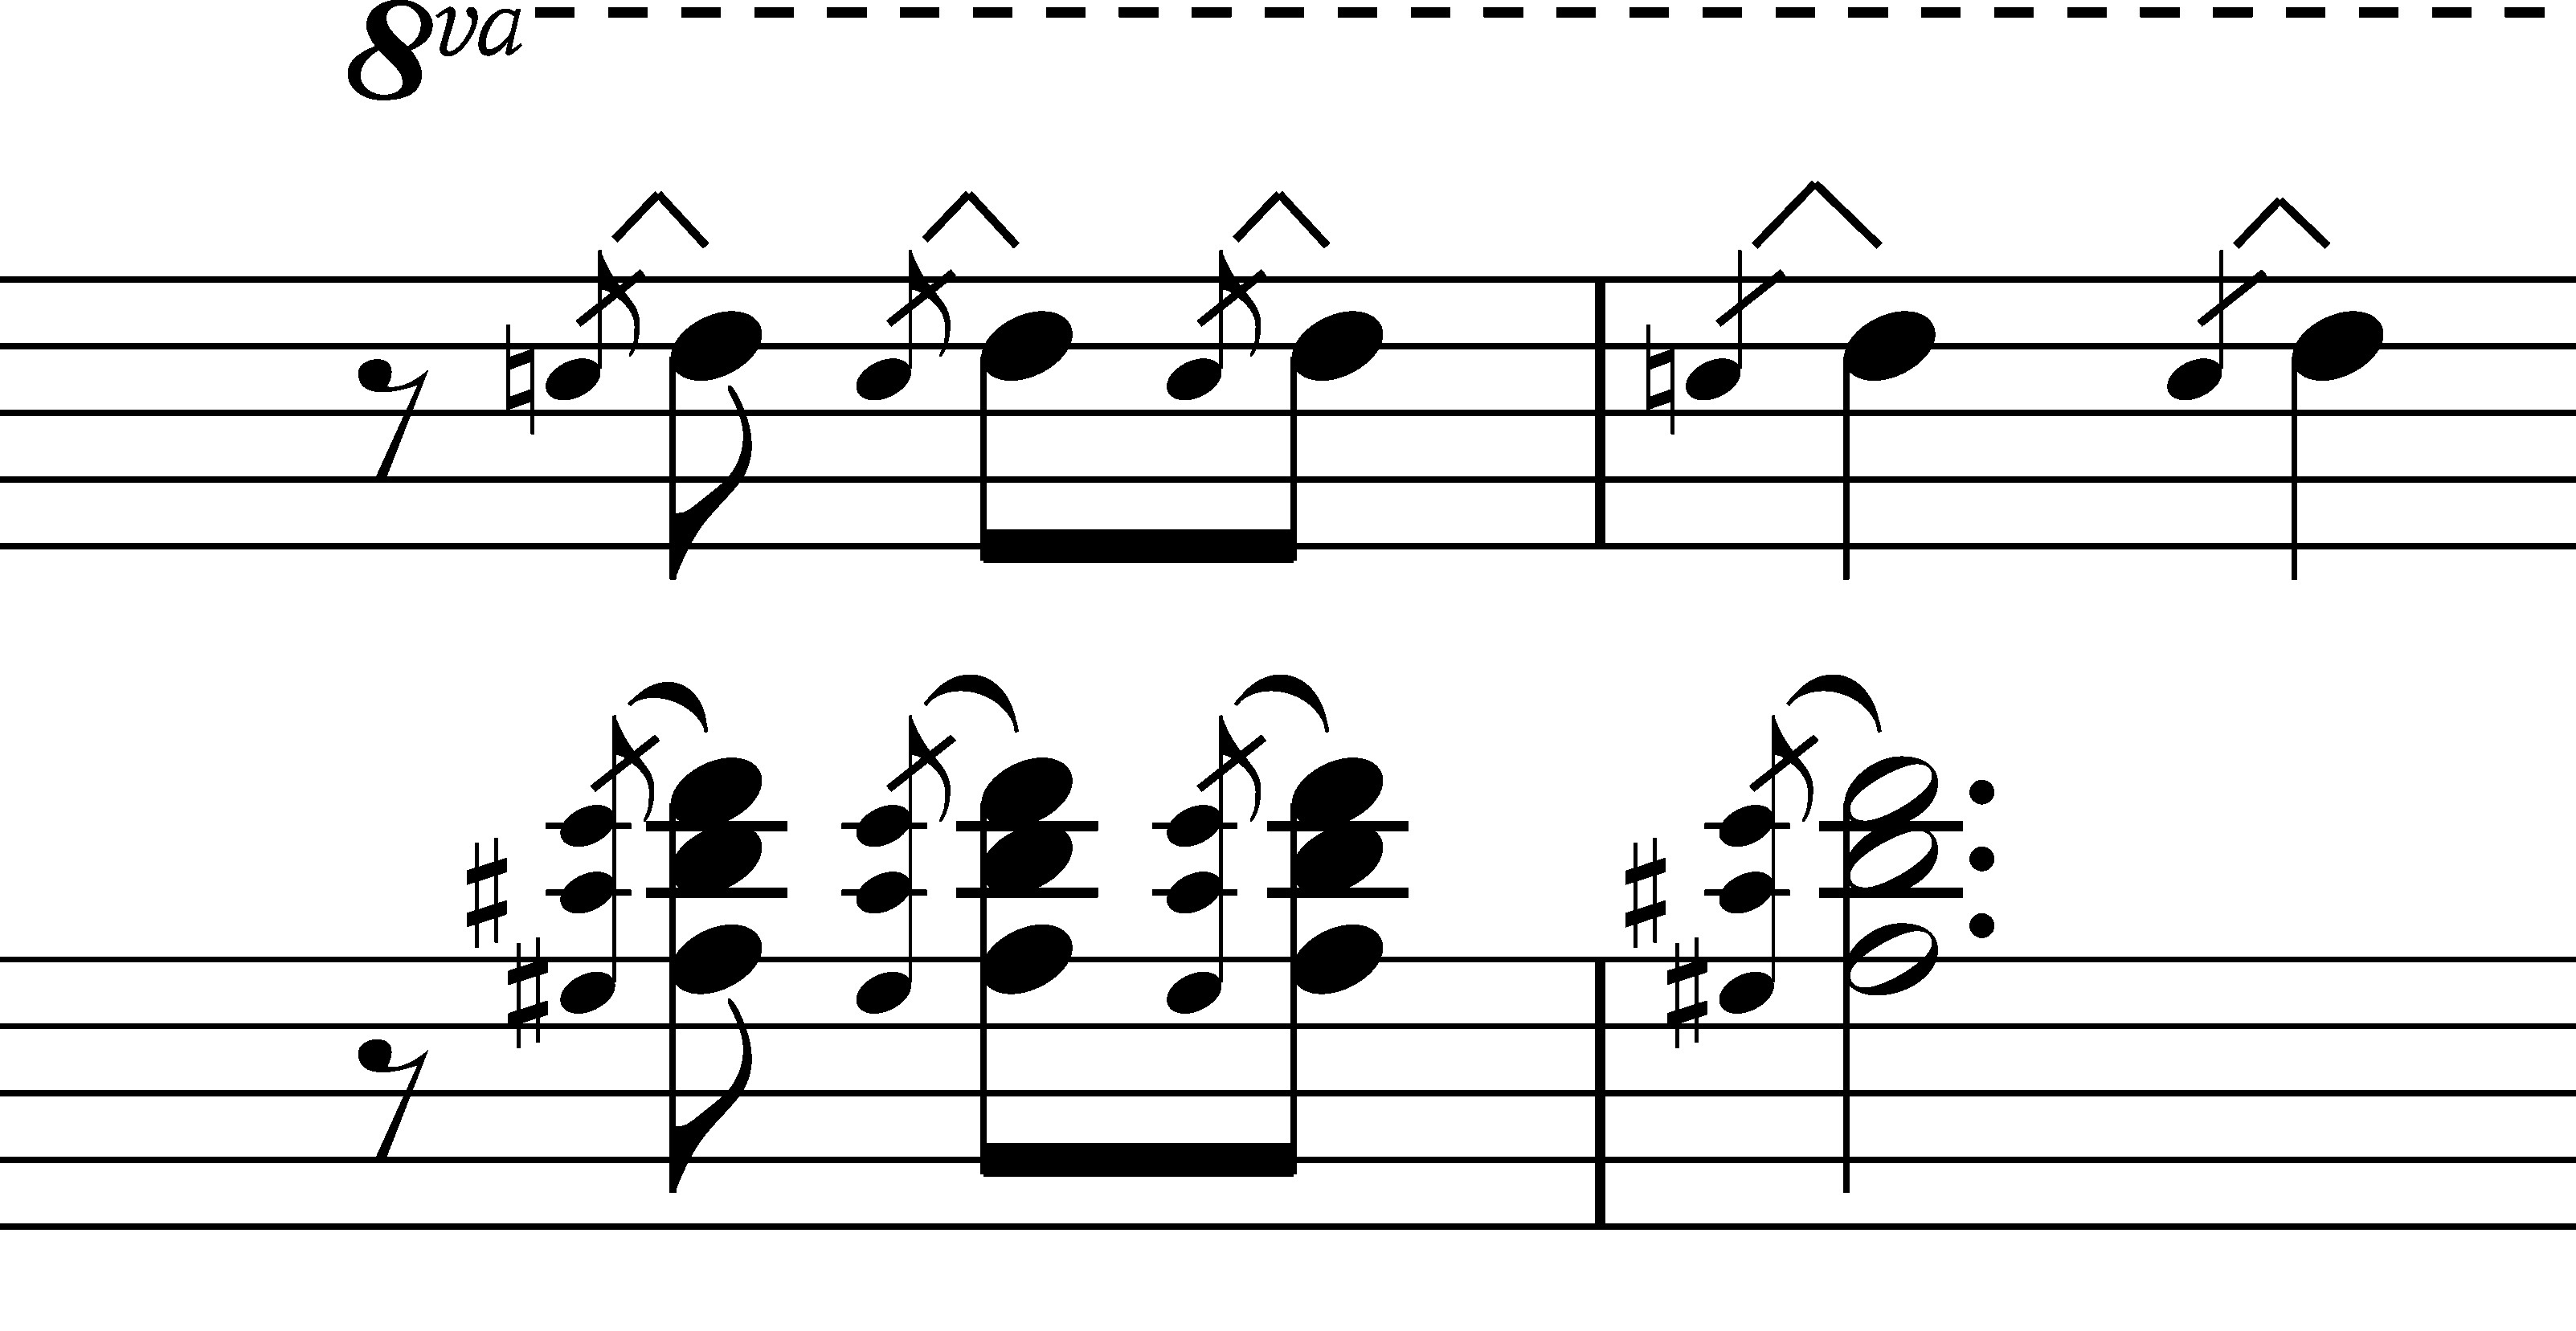
\includegraphics[width=\textwidth,keepaspectratio]{guitars/guitChoir}
  \subcaption{Lancio del solo, minuto \(3:25\)}
 \end{minipage}
 \hfill
 \begin{minipage}{0.4\textwidth}
  \centering
  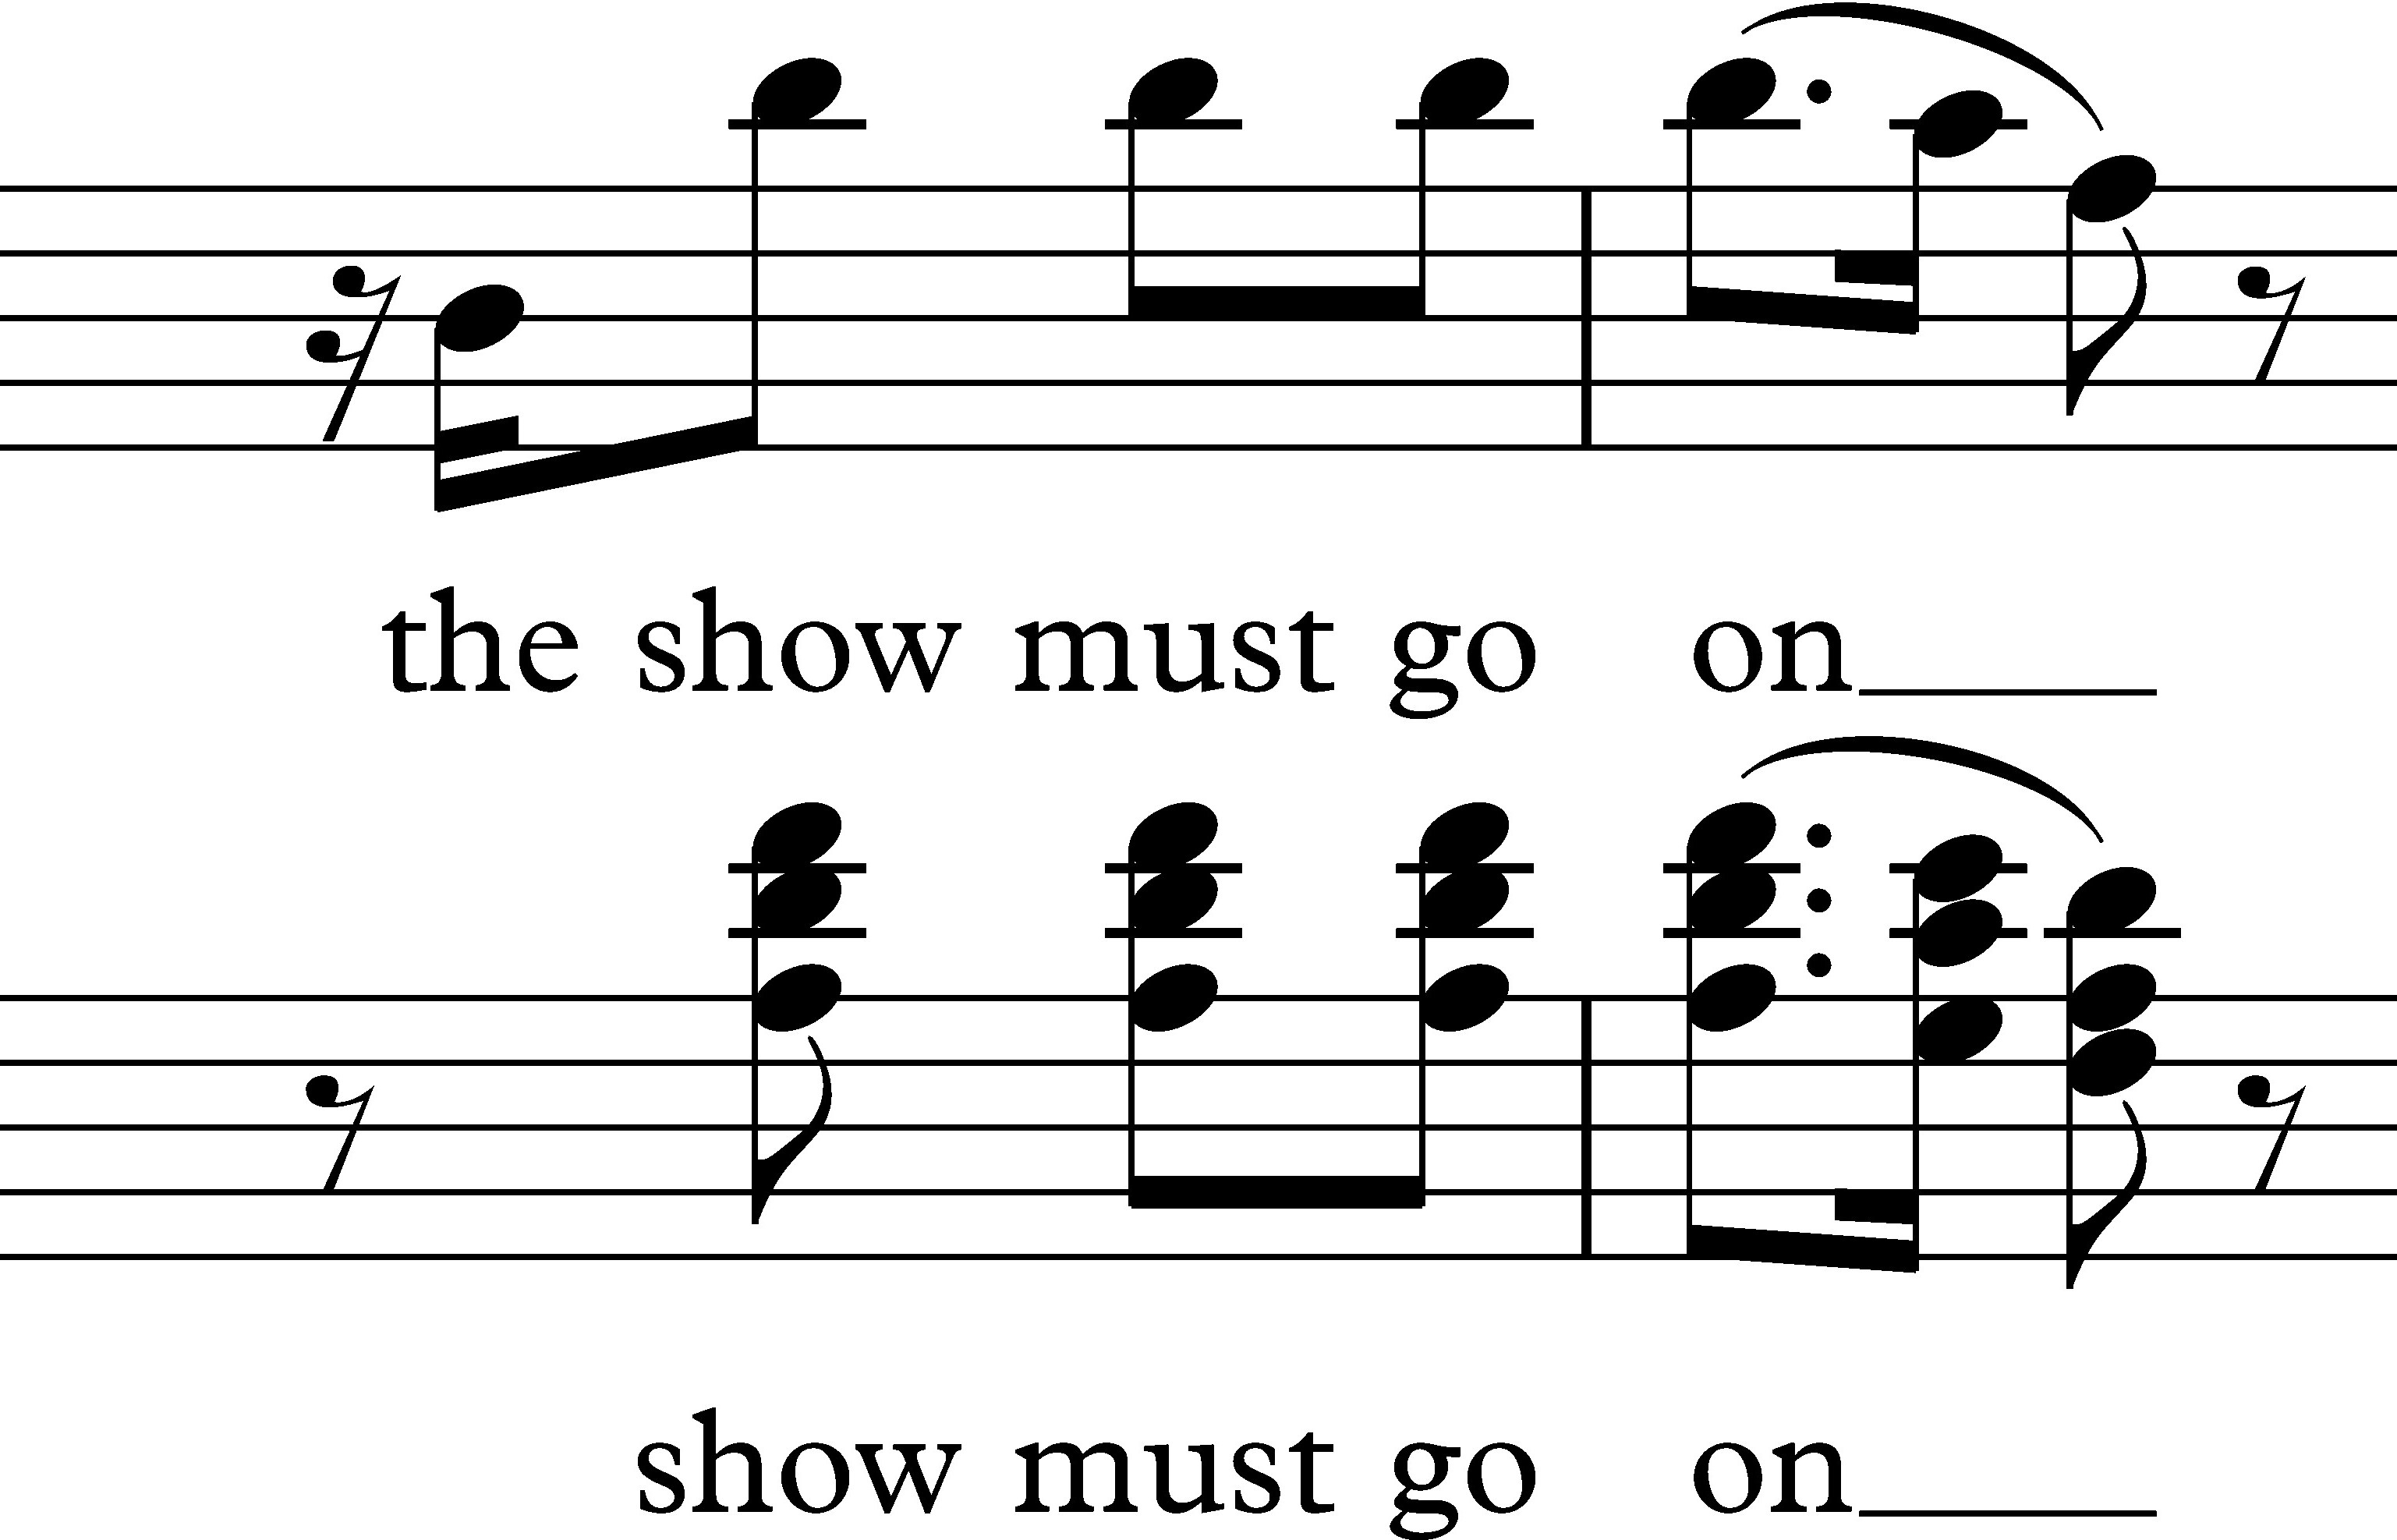
\includegraphics[width=\textwidth,keepaspectratio]{guitars/ch_guit}
  \subcaption{Voce e cori all'inizio del ritornello}
 \end{minipage}
\end{figure}

\subsubsection{Basso}
Già dalla prima strofa possiamo trovare un esempio di come John Deacon, in assenza di un groove di batteria, cercasse un approccio melodico per la linea di basso, come già detto in~\ref{par:jdtech}; dallo spartito in figura~\ref{fig:bass1} si può notare l'uso della scala minore naturale e di accordi sospesi per i movimenti più ampi.

\begin{figure}[H]
 \centering
 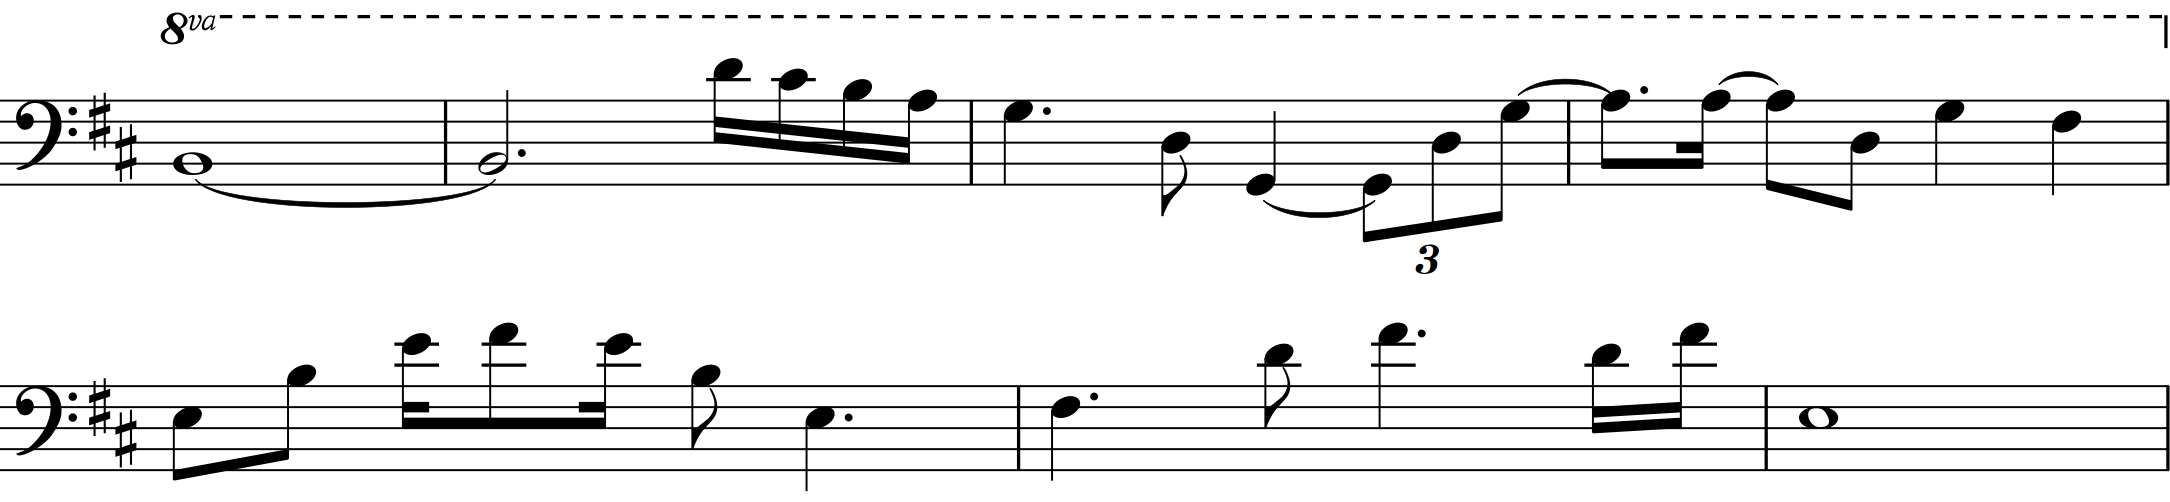
\includegraphics[width=\textwidth,keepaspectratio]{bass/bass1}
 \caption{Linea di basso, da \(0:19\)}
 \label{fig:bass1}
\end{figure}

Con l'ingresso del groove di batteria nel ritornello, Deacon decide di supportarlo ribattendo le toniche (o anche le ottave) a quartine di ottavi, talvolta colpendo solamente l'ultimo elemento della quartina; è un accompagnamento molto semplice che tuttavia risulta efficace e ben si presta a servire la parte di tastiera che, come abbiamo visto, presenta la medesima figura ritmica.

Deacon non dimentica di fare dei piccoli fill in sedicesimi di quando in quando, e nei momenti più concitati e virtuosistici dei soli di chitarra si assicura di tenere alto il tiro raddoppiando il groove e andando in quartine di sedicesimi (figura~\ref{fig:bass2-3}).

\begin{figure}[H]
 \centering
 \begin{minipage}{0.4\textwidth}
  \centering
  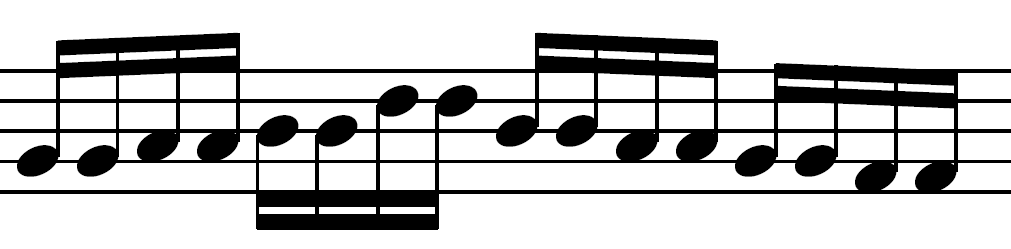
\includegraphics[width=\textwidth,keepaspectratio]{bass/bass2}
  \subcaption{Minuto \(2:37\)}
 \end{minipage}
 \hfill
 \begin{minipage}{0.4\textwidth}
  \centering
  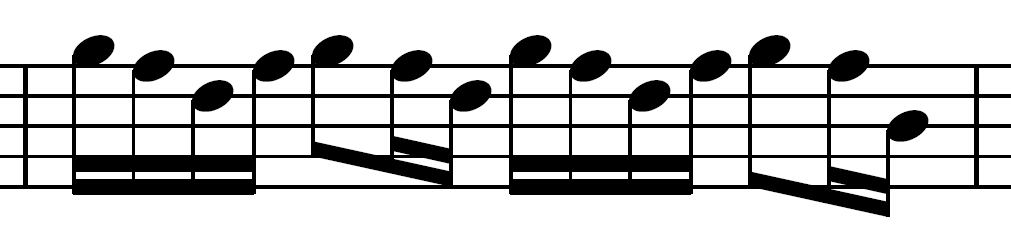
\includegraphics[width=\textwidth,keepaspectratio]{bass/bass3}
  \subcaption{Minuto \(3:34\)}
 \end{minipage}

 \caption{Esempi di linee di basso durante i soli}
 \label{fig:bass2-3}
\end{figure}

\subsubsection{Batteria}
Uno degli elementi più notevoli legati alla traccia di batteria è certamente la scelta dei suoni di produzione. È subito evidente infatti, anche senza l'ausilio di un multitraccia, l'uso fatto sui rullanti di riverberi estremamente ampi e lunghi, quasi da cattedrale, per ottenere un suono spesso e potente. Questo era un tratto ampiamente diffuso nelle produzioni rock e hard rock degli anni '\(80\), ed è certamente uno degli elementi che più distingue il suono del genere in quel periodo: basti pensare alle batterie dei dischi di artisti come Bryan Adams, Bon Jovi, Def Leppard, Europe, Skid Row e moltissimi altri.

In questo pezzo Roger Taylor sceglie di usare un pattern ritmico molto semplice, che mantiene per per l'intera durata del brano senza variazioni sostanziali. Possiamo ipotizzare che questa decisione sia stata presa con l'intento di servire al massimo la canzone e lasciare quanto più spazio possibile alla voce di Mercury: se infatti Taylor si fosse avventurato in fill importanti e pattern ritmici esotici, forse sarebbe andato a oscurare la traccia vocale. indipendentemente da quale possa essere stato il motivo della scelta di Taylor, questo si traduce in un groove solido e definito, una perfetta ossatura ritmica arricchita dalle trame del basso e dei synth.

Tra i pochi sgarri che Taylor si concede il più notevole è senza dubbio il fill che occorre nella terza misura del pezzo (figura~\ref{fig:drums}). Di per sé sono quattro colpi sui tom, ciascuno della durata di un ottavo puntato, ma ciò che li trasforma una perfetta \emph{ouverture} per il pezzo è che il primo colpo cade sul secondo elemento della seconda quartina di sedicesimi della misura. Il levare del sedicesimo, infatti, richiama subito l'attenzione dell'ascoltatore, e al contempo gli veicola efficacemente la solennità del brano che sta per apprezzare.

\begin{figure}[H]
 \centering
 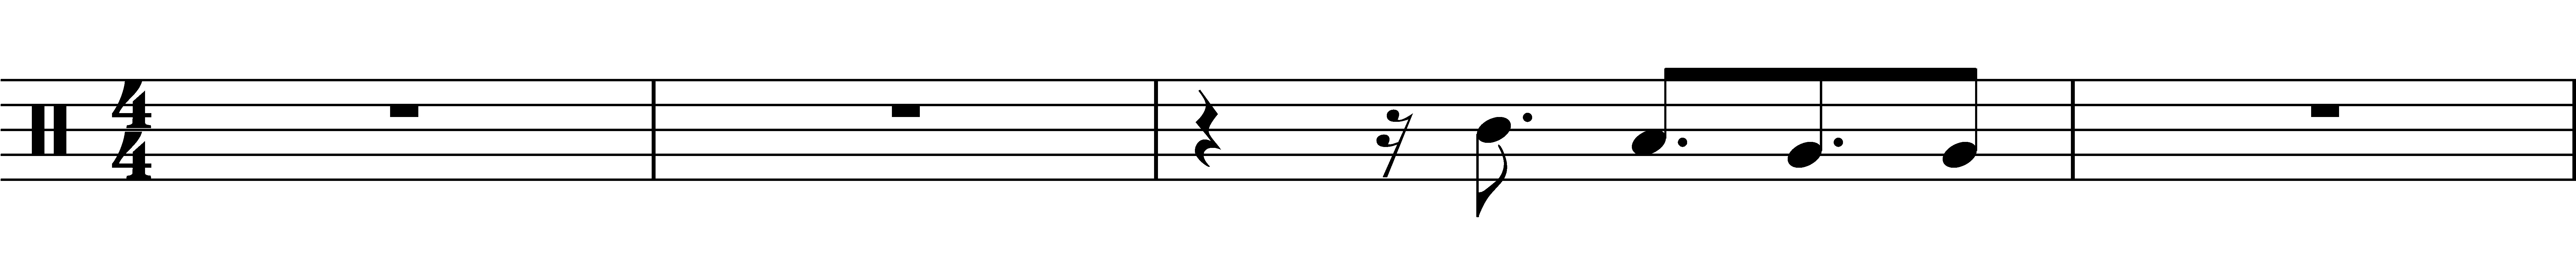
\includegraphics[width=\textwidth,keepaspectratio]{drums/drums}
 \caption{Fill iniziale, minuto \(0:06\)}
 \label{fig:drums}
\end{figure}

\section{Analisi armonica}
The Show Must Go On presenta uno sviluppo armonico di per sé relativamente semplice, dal momento che il pezzo è costruito in quasi la sua interezza attorno a un unico giro armonico. Ciononostante, questo singolo giro armonico, se visto attraverso occhi sufficientemente curiosi, può rivelare numerosi particolari degni di nota. Inoltre, come da tradizione Queen, sono presenti ben due piccole modulazioni, che contribuiscono a rendere il pezzo meno armonicamente statico.

\subsection{Generalità}

Iniziamo dicendo che il brano è scritto nella scala di \emph{SI minore naturale}, con numerosi prestiti da \emph{SI minore armonico}, ed è marcatamente tonale.

L'introduzione del pezzo presenta, fin da subito, il giro armonico principale del pezzo che, semplificando, presenta una progressione di questo tipo: Im | Im | \(\flat\)VI | \(\flat\)VI | IVm\(^{7}\) | V | IVm VII\textsuperscript{o}/IV, anche se avremo molto da dire soprattutto su quell'ultimo accordo.

\subsection{Il movimento delle voci}
La prima idea che sentiamo nella progressione è il marcato movimento interno agli accordi. Osserviamo subito come le prime due battute, entrambe un Bm in primo rivolto, ogni \(\frac{2}{4}\) muovano la voce: inizialmente scende di un semitono e colpisce la sopratonica/seconda, successivamente sale di un tono e mezzo per colpire la sottodominante/quarta, per poi tornare nelle ultime due pulsazioni sulla voce di partenza. Quando, nella terza e quarta battuta del giro, si passa a un G, la figura e le note colpite restano invariate, e quindi la voce mobile in questo caso diventa la dominante/quinta dell'accordo. La figura si ripete immutata anche nella quinta misura con un Em7, con la voce sulla settima di dominante (quindi, di nuovo, da un RE si passa a un DO\(\sharp\)); nella sesta misura, invece, vengono mosse delle voci interne all'accordo, in modo da comporre prima un F\(\sharp\)\textsuperscript{(sus\(4\))} e, conseguentemente, un F\(\sharp\). Un ultimo movimento lo abbiamo nella settima misura del giro, quando la voce sulla dominante del Em viene abbassata di un semitono, formando un accordo che, per questioni di spelling, andrebbe correttamente notato come A\(\sharp\)\textsuperscript{dim}/E.

\begin{figure}[H]
 \centering
 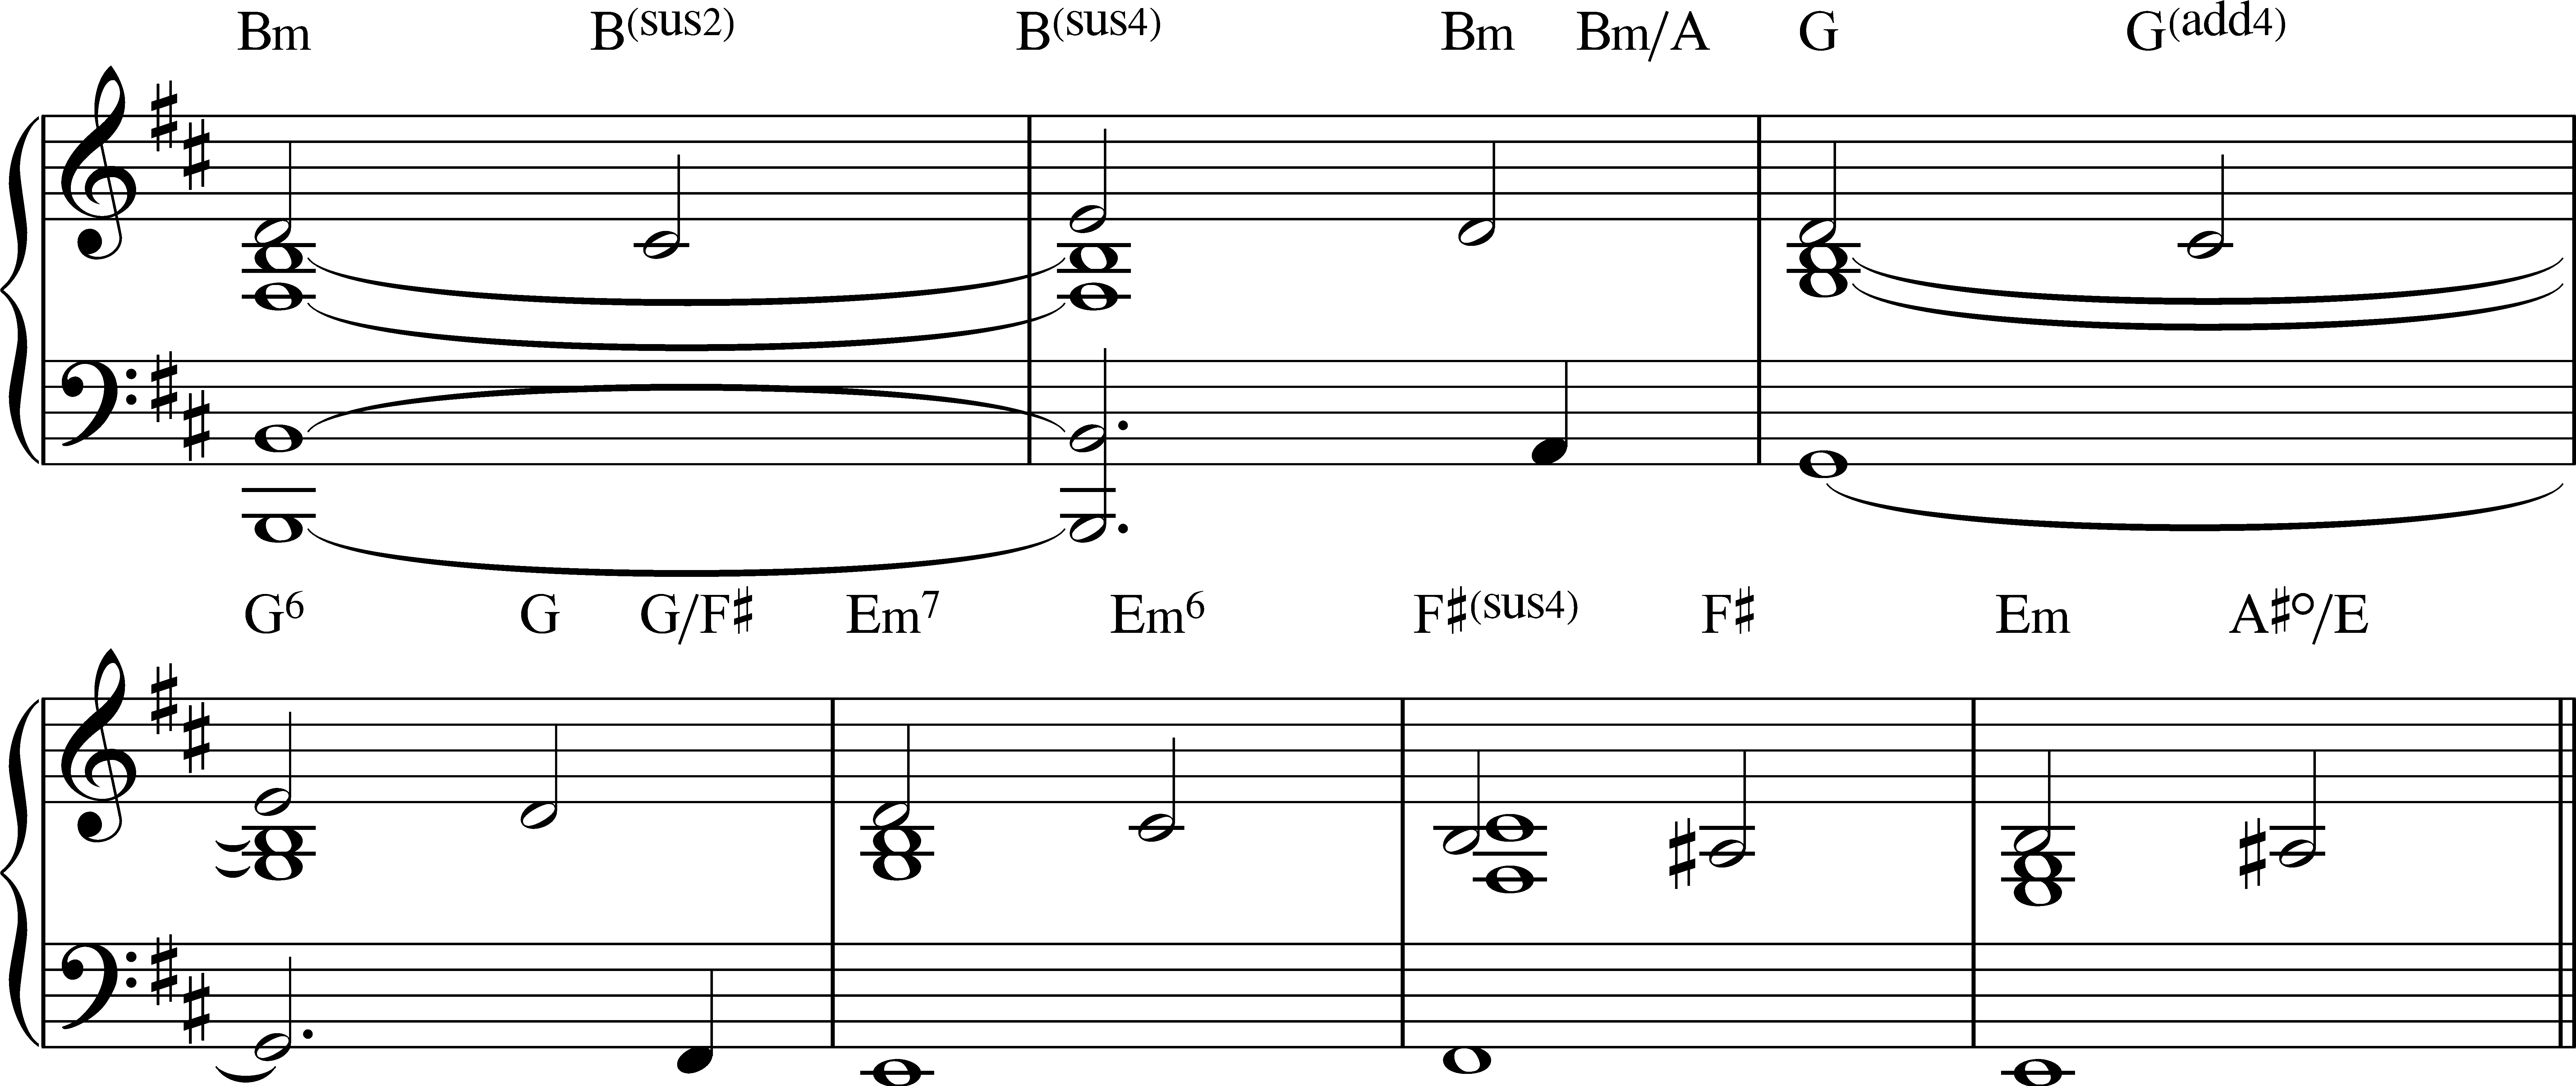
\includegraphics[width=\textwidth,keepaspectratio]{aa/main-progression}
 \caption{Progressione principale del brano}
 \label{fig:progression}
\end{figure}

Quest'idea è molto utile per rendere più mobili e interessanti situazioni armoniche che, altrimenti, risulterebbero molto statiche, dal momento che si parla di accordi che ricoprono intereramente due misure a una velocità relativamente bassa (circa \(84\) bpm). Non è certamente nuova: di nuovo, la si può ritrovare nei Beatles in \emph{Norwegian Wood}, dove in realtà vediamo lo sviluppo di una vera e propria linea melodica sopra a un accordo che funge quasi da pedale. È stata ripresa e usata estensivamente nella musica folk e in generale in tutti i generi prevedessero l'uso di una chitarra acustica, considerata la semplicità con cui un chitarrista può eseguire questi passaggi con gli accordi D e A in prima posizione. Negli anni '\(80\) la troviamo, tra gli altri, nel ritornello della celeberrima \emph{Summer of '69} di Bryan Adams, in \emph{Runaway} dei Bon Jovi e in \emph{Prisoners in Paradise} degli Europe. La si può trovare anche in alcuni contesti metal, come in \emph{Mary Lou} dei Sonata Arctica.

\subsection{Analisi funzionale}
Parallelamente al movimento delle voci avviene la progressione coi macromovimenti armonici veri e propri. Questi sono raccordati dalla linea di basso che, nella pulsazione che precede i cambi, suona quella che sarebbe stata la fondamentale dell'accordo di passaggio. Questo moto discendente dona alla progressione una forte direzionalità.

La progressione inizia con un Im, accordo di tonica e che stabilisce subito il centro tonale in SI minore, anche se naturalmente non possiamo ancora essere certi che il brano sia costruito in modo tonale; ad ogni modo, quando durante lo sviluppo del brano vengono cercate delle risoluzioni, queste cadranno sempre sul Bm (ad esempio nella chiusura del primo ritornello o nel finale stesso), e in tutti quei contesti possiamo inequivocabilmente rilevare che quell'accordo veicola all'ascoltatore un senso di relativo riposo ed equilibrio, nonostante naturalmente un accordo minore risulti meno stabile di uno maggiore.

Muovendosi dalla tonica, gli accordi che vengono successivamente colpiti sono un \(\flat\)VI e un IVm\(^{7}\); questi due accordi, entrambi sottodominanti, portano l'ascoltatore via via più lontano dal luogo di riposo e, a causa del moto discendente del basso, questo viaggio assume una forte aura di gravità e oppressione, quasi come se la progressione armonica stesse cercando di trasportare l'ascoltatore nell'abisso fisico ed emotivo in cui la malattia aveva verosimilmente gettato Mercury stesso.

A seguito del IVm\(^{7}\) troviamo un V\textsuperscript{(sus\(4\))}, seguito immediatamente da un V; questo è un'istanza di interscambio modale dalla scala minore armonica di SI, dal momento che l'accordo costruito sul quinto grado di una scala minore naturale dovrebbe essere minore, ma il settimo grado aumentato di un semitono (un LA\(\sharp\) al posto di un LA) rende l'accordo maggiore. Questo schema è stato usato fin dalle origini della musica occidentale proprio a causa della grande tensione che genera, perfetta per chiamare la risoluzione di un giro armonico; nella musica leggera la troviamo spesso come antecedente in una sorta di variazione di una cadenza d'inganno (V - Im in scala minore armonica al posto di V - VIm in scala maggiore), mentre invece in molti pezzi classici, a partire da Bach e poi estensivamente nei contesti ecclesiastici, era molto diffuso l'uso della cadenza piccarda, che consiste nel terminare una progressione in modo minore con un accordo di primo grado con la terza maggiore (per citare alcuni esempi moderni, si senta la cover di \emph{Black Betty} dei Ram Jam a \(0:31\) o \emph{Foreplay} dei Boston a \(1:23\)).

Ma in questo caso al V non segue una risoluzione, bensì l'armonia scende di nuovo di un tono e colpisce nuovamente un IVm, che normalmente ha una funzione sottodominante e riduce quindi la tensione creata dal precedente accordo. A questo punto ci si potrebbe aspettare una variante minore della cadenza plagale e quindi una soluzione dal IVm al Im, ma le aspettative dell'ascoltatore sono nuovamente sconvolte, perché prima dell'agognata soluzione compare un ultimo movimento: la voce in SI dell'accordo di Em viene abbassata di un semitono  a un LA\(\sharp\), producendo in questo modo che noi notiamo formalmente come un A\(\sharp\)\textsuperscript{o}/E. Le osservazioni su quest'ultimo movimento sono tali da meritare di essere approfondite in un paragrafo dedicato.

\subsection{Interpretazioni sulla funzione di A\(\sharp\)\textsuperscript{o}/E}
Normalmente, gli accordi costruiti sul IVm in una tonalità minore (o il IIm della relativa maggiore) hanno una funzione sottodominante, ed è con questa funzione che già li abbiamo incontrati precedentemente in quest'analisi. Ma nonostante questo, il compositore ha scelto di costruire qui l'apex della tensione del giro armonico del pezzo, e all'ascoltatore risulta efficace, poiché quest'accordo assolve perfettamente la funzione dominante e ci riporta nella situazione di riposo della tonica Bm. Una prima spiegazione semplice si individua facilmente se si conosce come sono costruite le triadi diminuite.

% \paragraph{Sostituzione di F\(\sharp^{7(\flat9)}\)}
Nonostante l'uso di accordi diminuiti non sia molto diffuso nella musica leggera, i Queen ne avevano già usati in numerose occasioni, soprattutto nei pezzi armonicamente più interessanti (si veda, tra tutti, \emph{Bohemian Rhapsody} e \emph{We Are the Champions}).

Una triade diminuita è costituita dalla fondamentale, una terza minore e una quinta diminuita; nel nostro caso non è presente la terza minore, ma è presente la settima diminuita, sicché la funzione dell'accordo risulta molto simile (di fatto, si può dire che la nostra triade sia in realtà una quadriade diminuita senza la terza, infatti l'abbiamo notata come A\(\sharp\)\textsuperscript{o}/E anziché A\(\sharp\)\textsuperscript{dim}/E). In particolare, la quinta diminuita e la fondamentale formano il tritono, un intervallo particolarmente instabile, ed è proprio questo a creare la tensione nella triade diminuita. Se poi osserviamo le singole voci ci accorgiamo che il LA\(\sharp\) vuole risolvere in alto sul SI, il SOL chiama il FA\(\sharp\) in basso e il MI in basso verso il RE.

Di fatto, questo accordo sostituisce un F\(\sharp^{7(\flat9)}\). Se infatti prendiamo un F\(\sharp\), possiamo estenderlo e trovare prima una MI (settima) e successivamente un SOL (bemol nona); opportunamente rivoltato, possiamo spostare il MI al basso ed eliminare dall'accordo il DO\(\sharp\) (quinta) e il FA\(\sharp\), rimanendo così con le tre note che compongono il nostro A\(\sharp\)\textsuperscript{o}/E. Quindi, secondo questa visione, altro non si tratterebbe che di una cadenza d'inganno.

L'idea funziona, ma c'è una seconda interpretazione che possiamo elaborare sfruttando un espediente compositivo recentemente comparso nella scena jazz: l'armonia negativa.

\subsubsection{Cos'è l'armonia negativa}
L'armonia negativa (tradotto letteralmente dall'inglese \emph{negative harmony}), nonostante il nome esotico, altro non è che un interessante approccio all'armonia portato in scena recentemente dal musicista britannico \emph{Jacob Collier}; in particolare Collier sostiene di averlo ripreso dal libro \emph{A Theory of Harmony} del compositore e musicologo svizzero \emph{Ernst Levy}, nel \(1985\).

Semplificando molto il discorso teorico di Levy, possiamo affermare che l'idea che sta dietro all'armonia negativa è che, data un determinato centro tonale, si possa individuare una forte polarità tra uno sviluppo "positivo" - per così dire - delle frequenze appartenenti a quel centro tonale, e uno sviluppo invece "negativo". La natura di questa polarità sarebbe pervasiva e molto profonda, dal momento che Levy arriva ad applicarla anche alla serie degli ipertoni e a quella degli ipotoni come sua rifrazione negativa (si può individuare un curioso parallelismo tra i concetti di \emph{Otonality} e \emph{Utonality} elaborati da \emph{Harry Partch}), ma in questa sede non abbiamo spazio per approfondire un argomento così complesso.

\paragraph{Come applicare la rifrazione}
\begin{wrapfigure}{L}{.4\textwidth}
 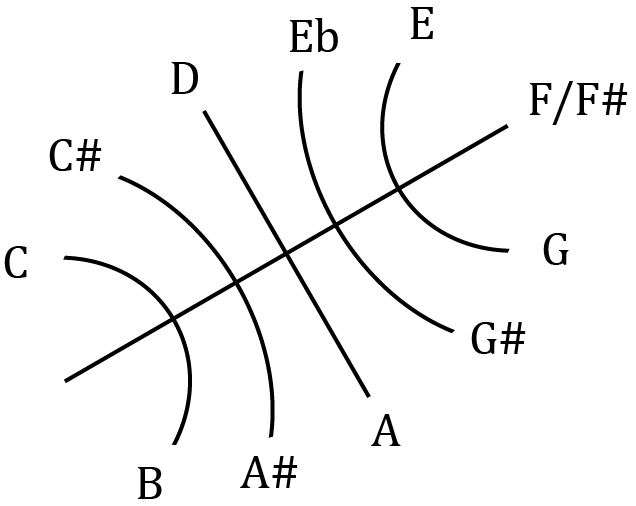
\includegraphics[width=\linewidth]{aa/na-circle}
 \caption{Asse di rifrazione in RE maggiore}
 \label{fig:na}
 \centering
\end{wrapfigure}

Quindi, usando il RE maggiore come nostro riferimento, possiamo individuare la rifrazione negativa di ogni elemento della scala tracciando un ipotetico asse di rifrazione tra la tonica  - RE - e la dominante - LA - nel circolo delle quinte, dividendolo così in due semicerchi, ciascuno la rifrazione dell'altro. Una rappresentazione visiva alternativa è presentata in figura~\ref{fig:na}. È interessante notare come l'insieme di note che costituisce la rifrazione negativa del nostro RE maggiore si rivela essere, una volta opportunemente riordinato, un LA frigio; ancora più interessante, Levy stesso fa notare che se partiamo dalla nota LA (dominante di RE) e andiamo a scendere seguendo la stessa struttura intervallare della scala maggiore (T - T - ST - T - T - T - ST), otteniamo la stessa scala di LA frigio, come si può vedere in figura~\ref{fig:m-ph}.

\begin{figure}[H]
 \centering
 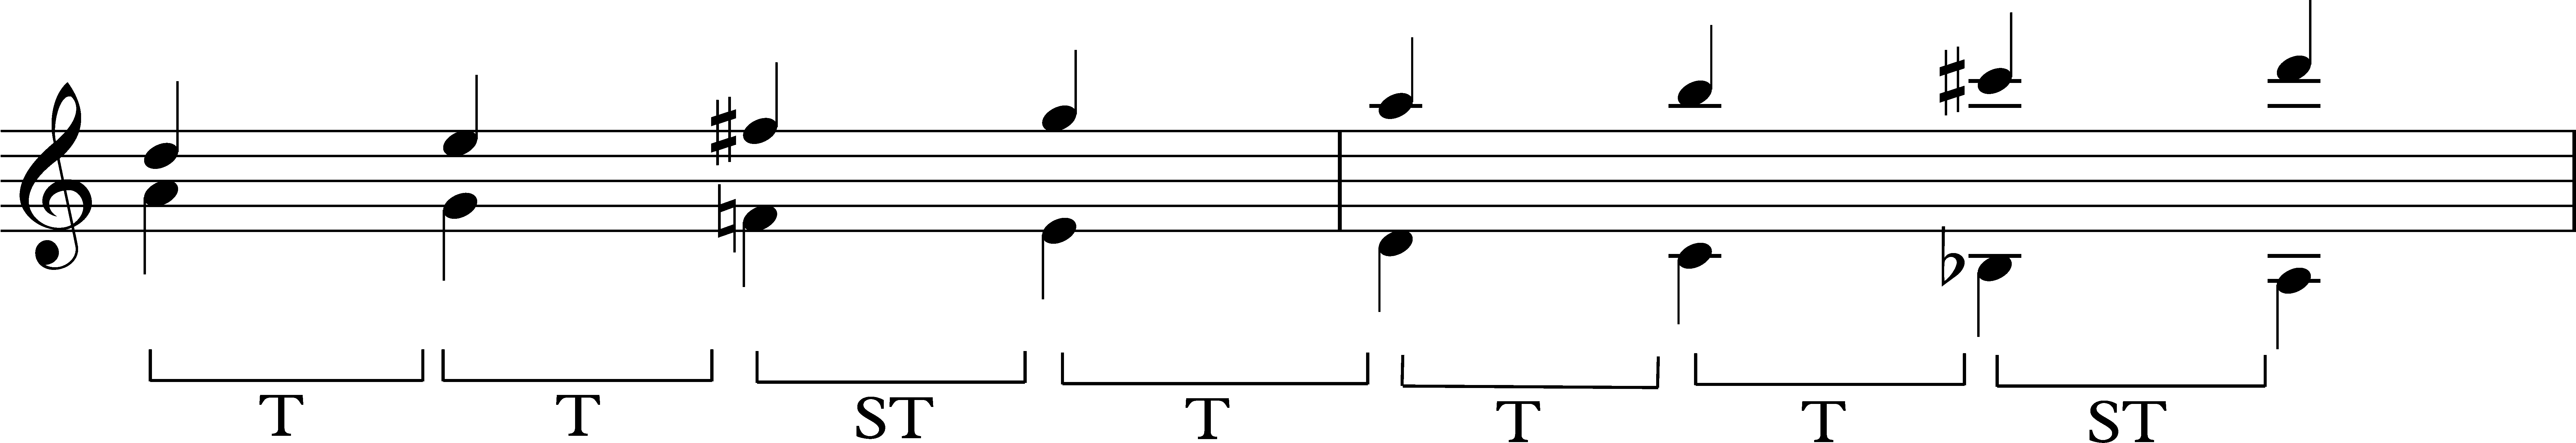
\includegraphics[width=\textwidth,keepaspectratio]{aa/major-phrygian}
 \caption{RE maggiore (sopra) e LA frigio (sotto) a confronto}
 \label{fig:m-ph}
\end{figure}

\paragraph{Applicazioni}
% \begin{wrapfigure}{R}{.45\textwidth}
%  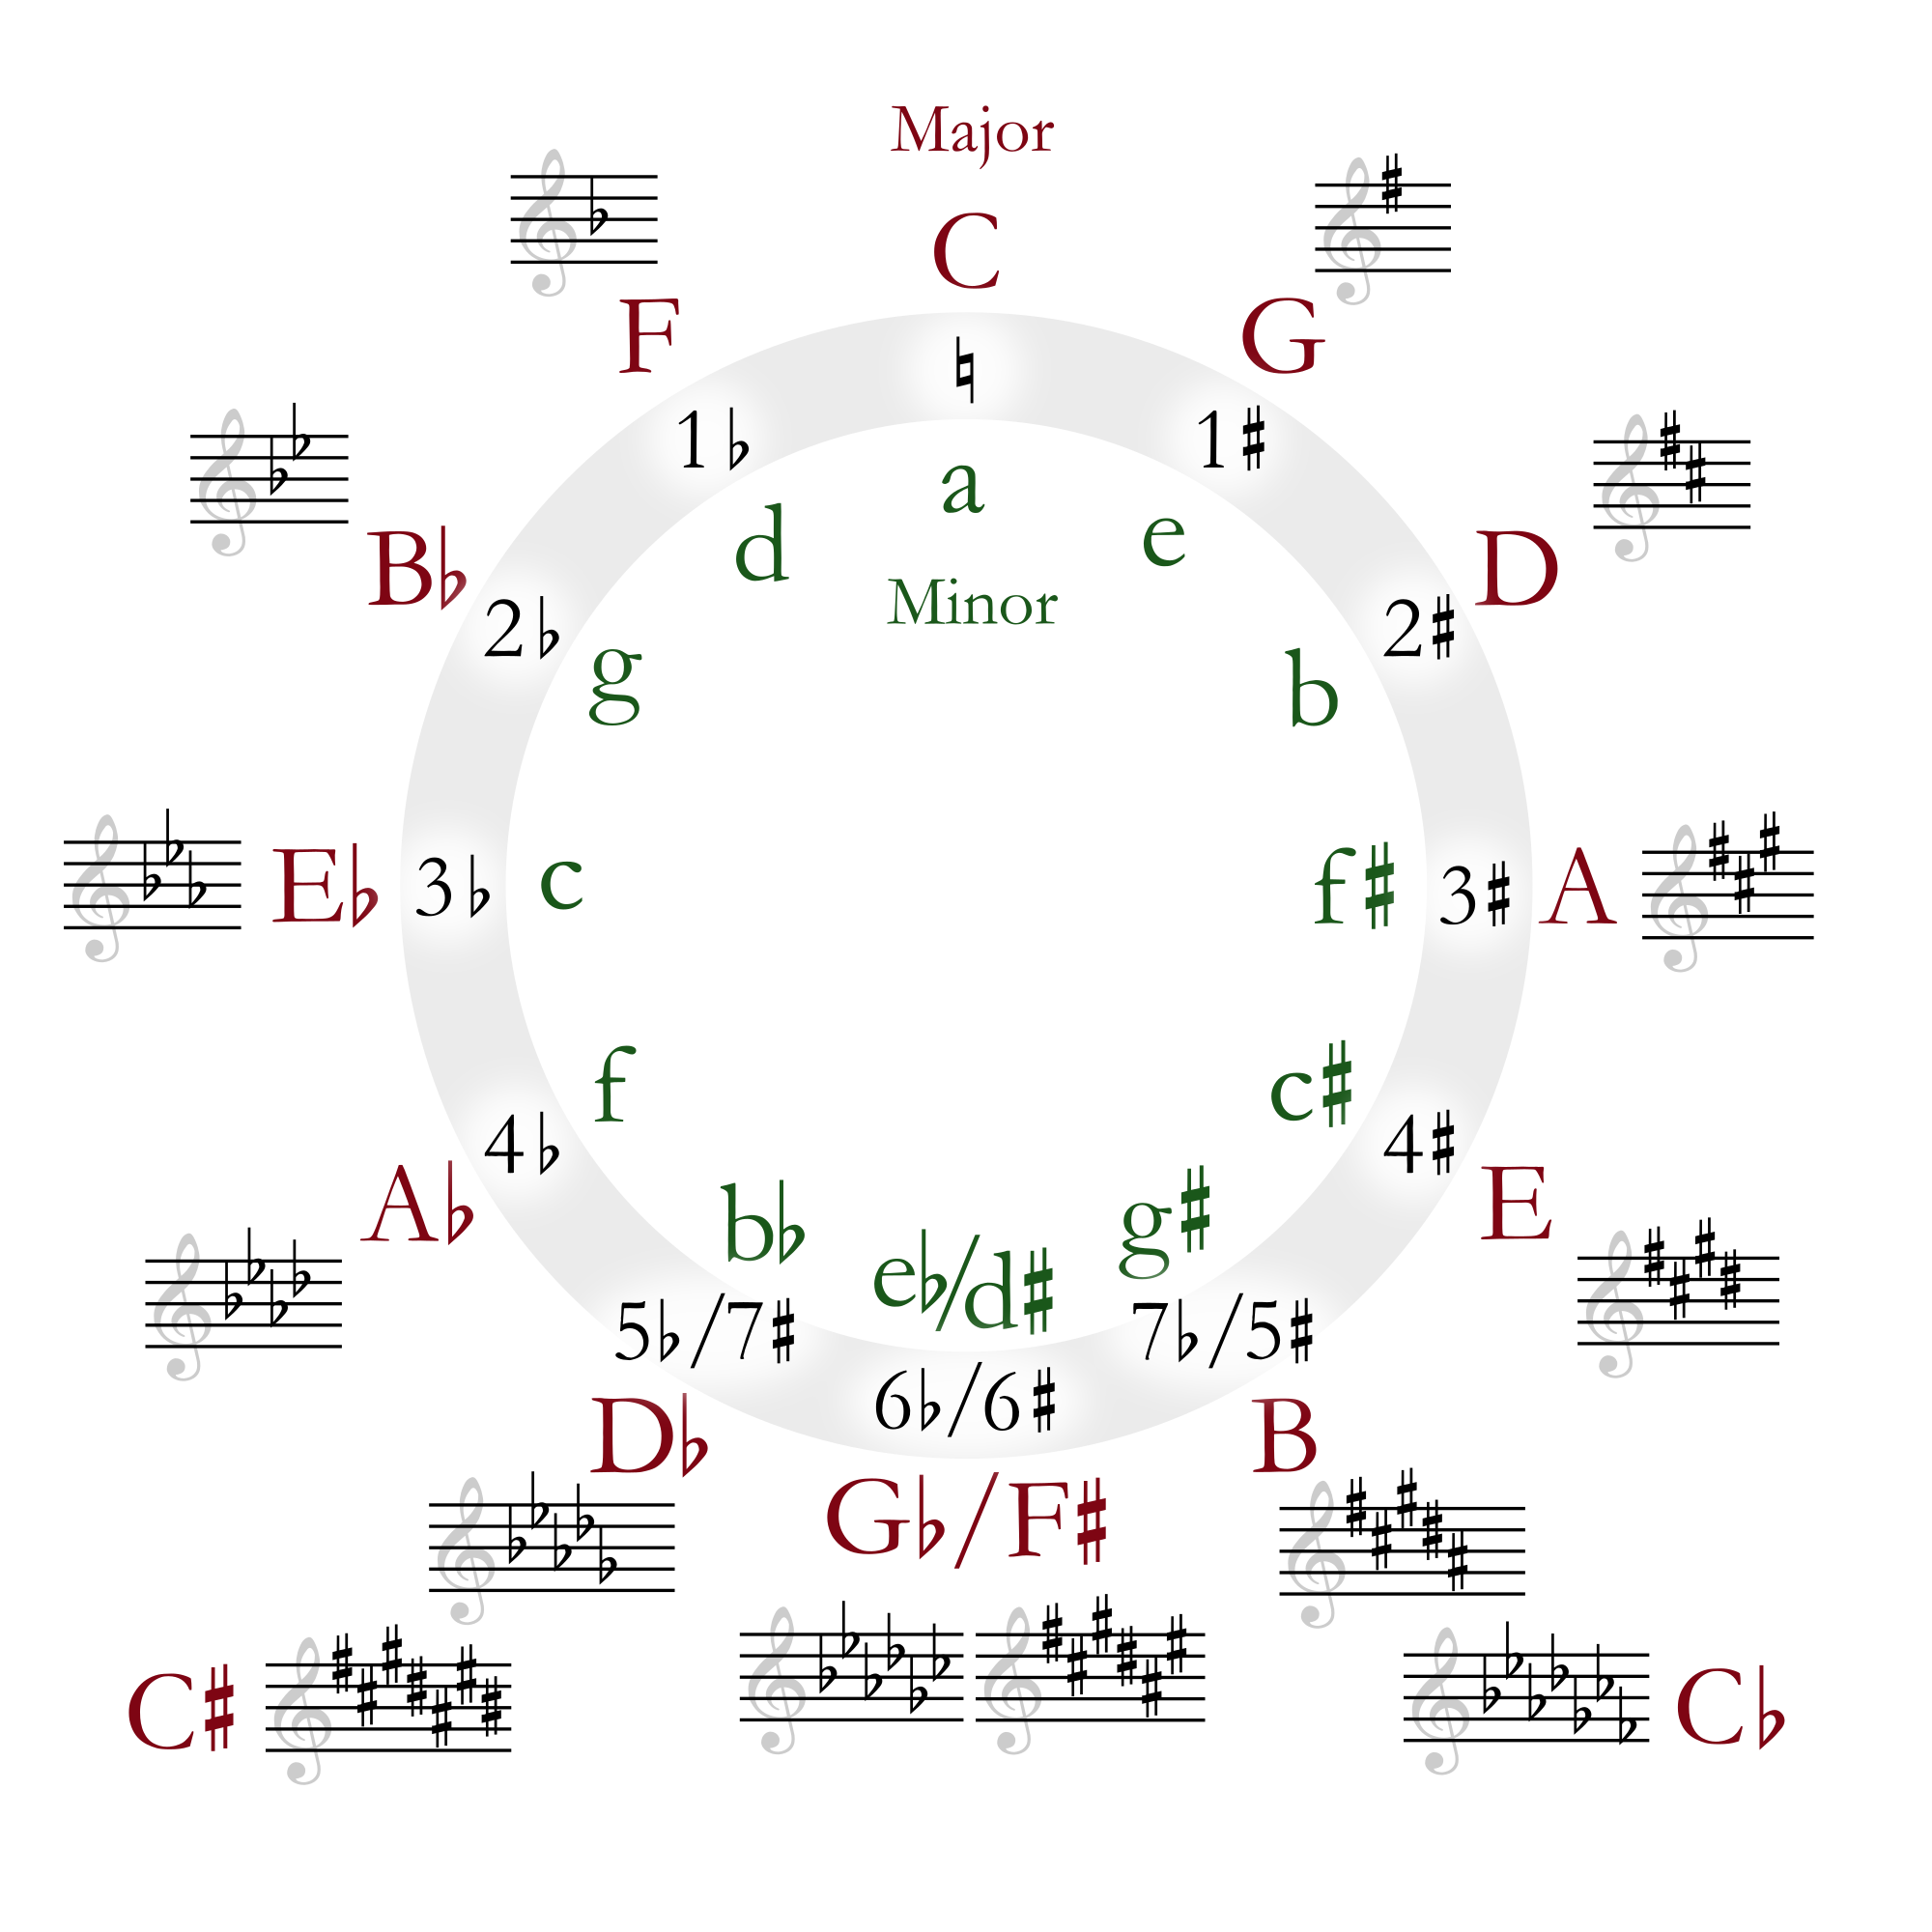
\includegraphics[width=\linewidth]{aa/circle}
%  \caption{Circolo delle quinte}
%  \label{fig:circle}
%  \centering
% \end{wrapfigure}

Quindi, l'applicazione pratica di questo interessante esercizio teorico sta nel fatto che è possibile raggiungere il medesimo obiettivo armonico (ad esempio una risoluzione) equialentemente sia dall'immagine positiva sia dalla sua rifrazione negativa: ad esempio, se consideriamo una progressione VI\(^{7}\) - II\(^{7}\) - V\(^{7}\) - I (una successione di cadenze perfette) in una qualsiasi tonalità notiamo che, sostituendo ogni nota alla corrispettiva rifrazione negativa, otteniamo il seguente risultato: \(\flat\)IIIm\(^{6}\) - \(\flat\)VIIm\(^{6}\) - IVm\(^{6}\) - I, una successione di cadenze plagali (si veda figura~\ref{fig:circle} per avere un riferimento visivo).

\begin{wrapfigure}{R}{.45\textwidth}
 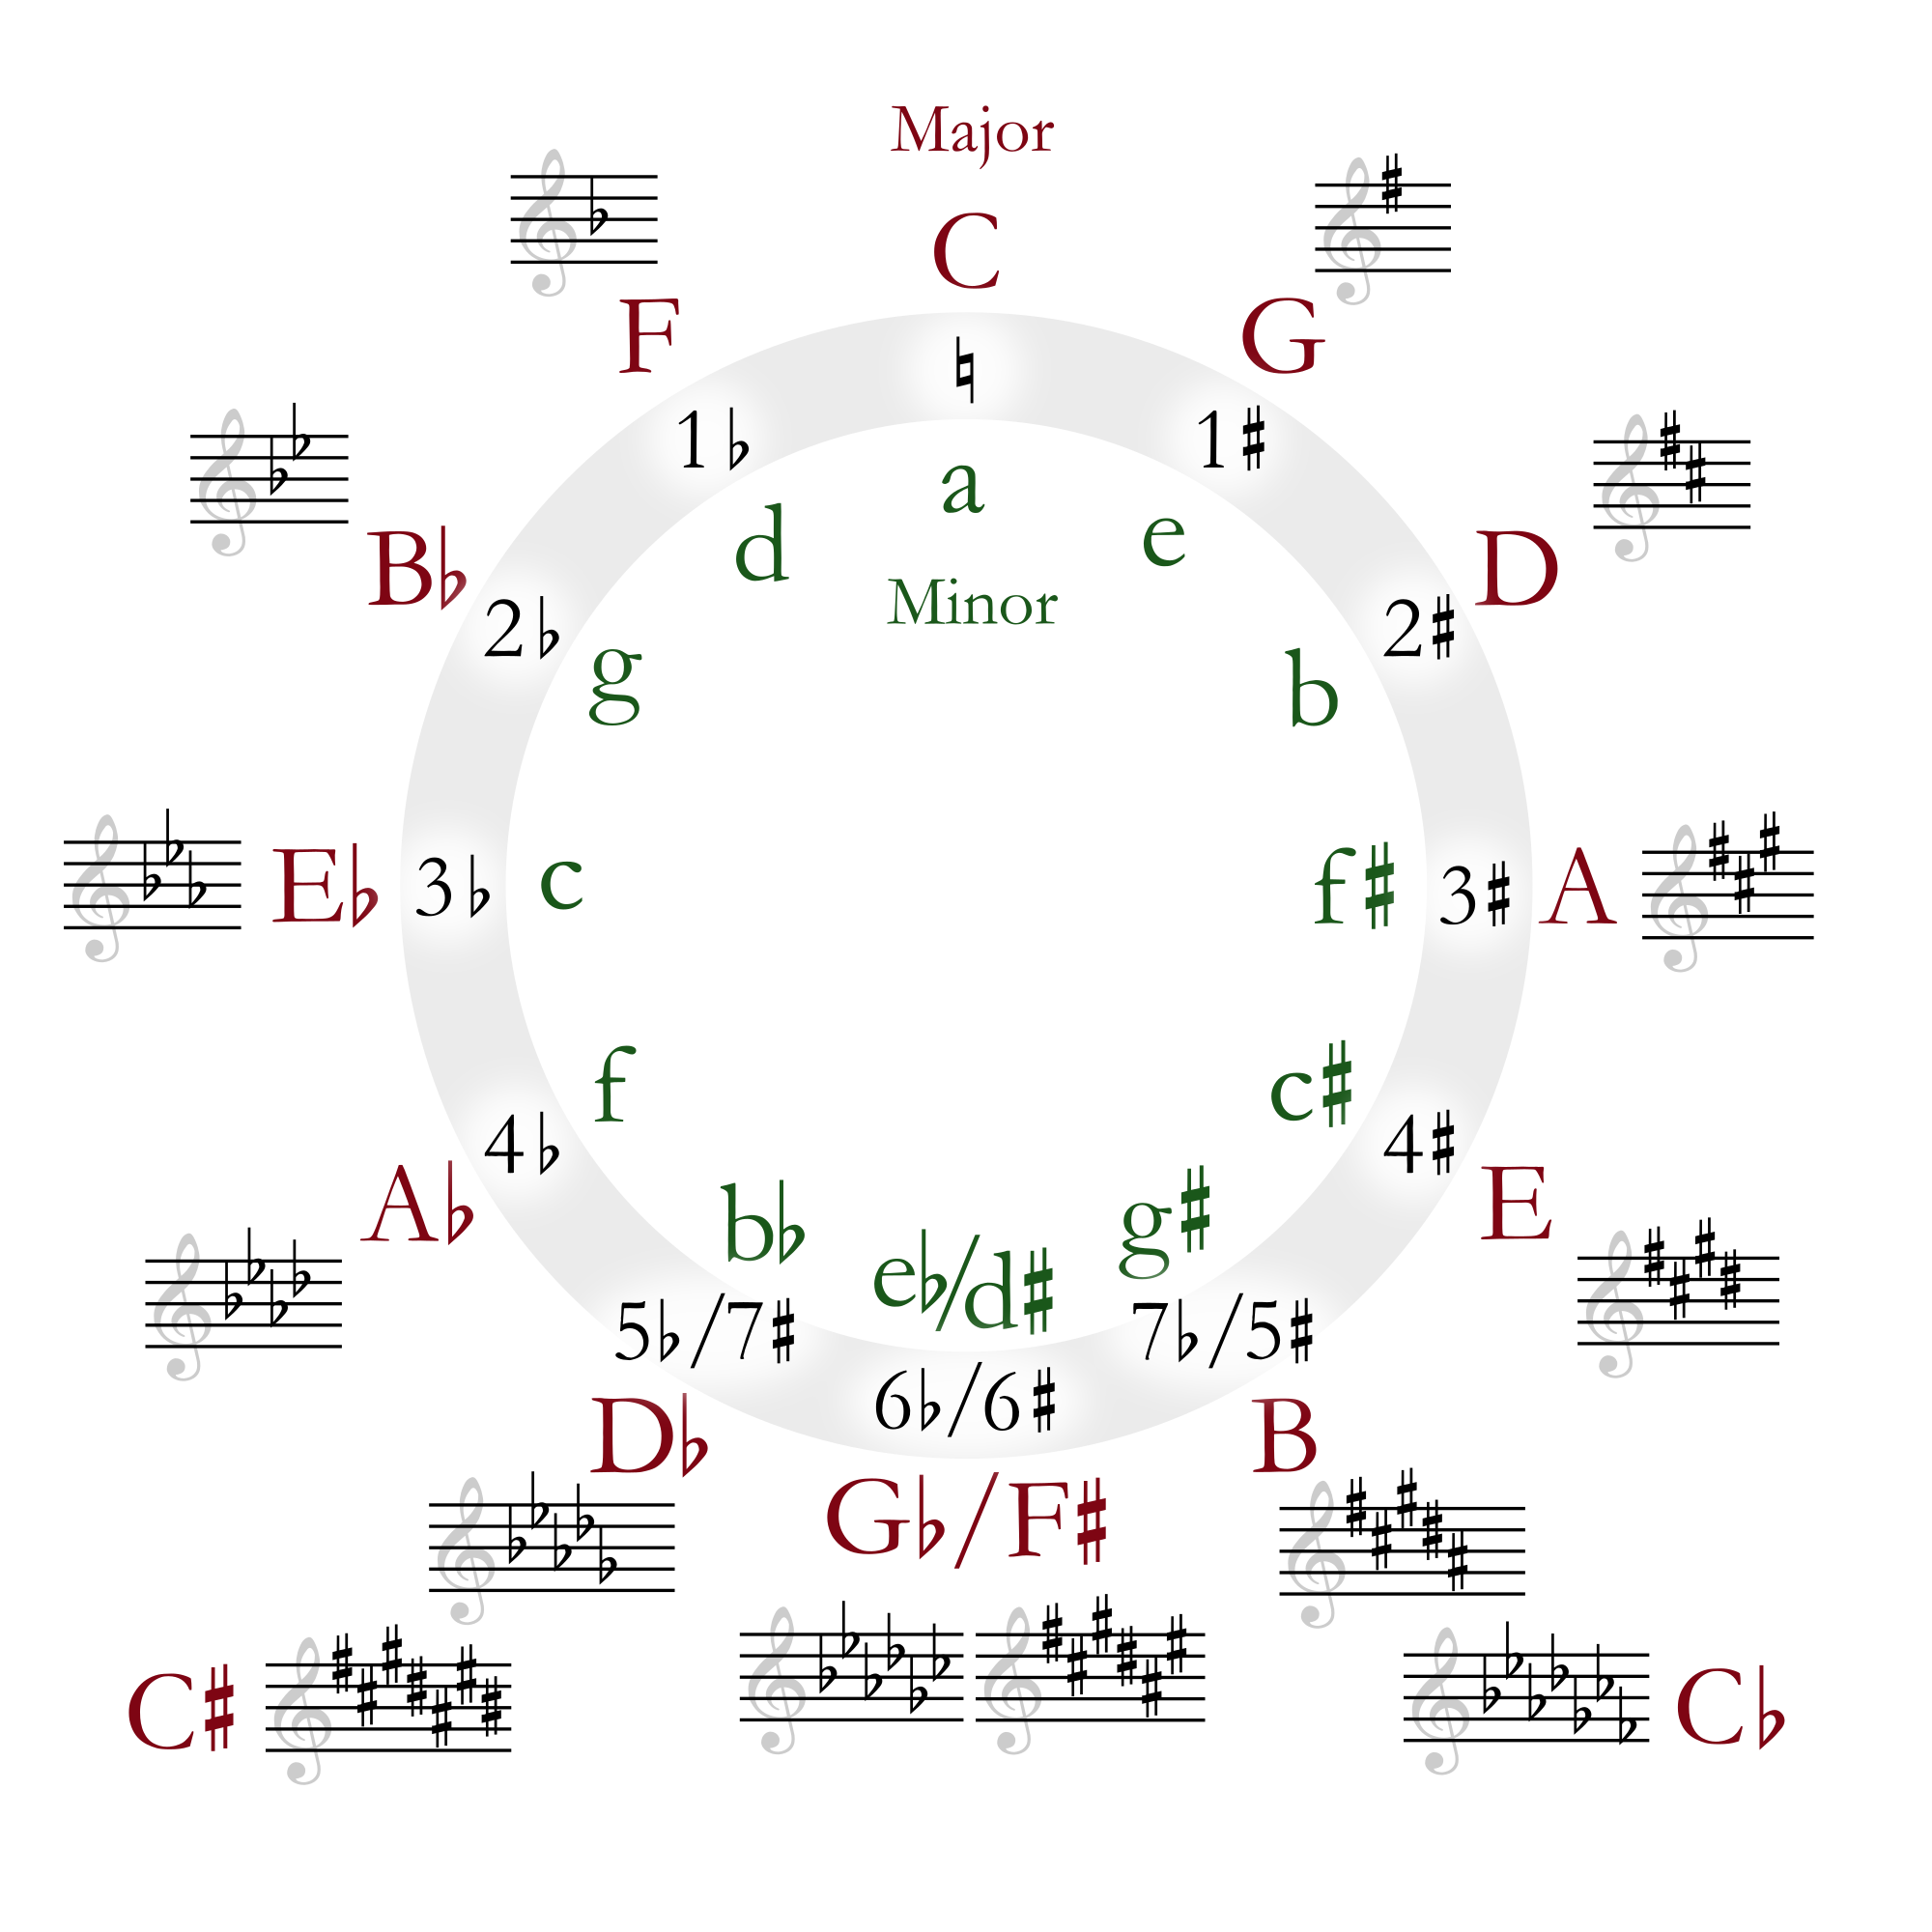
\includegraphics[width=\linewidth]{aa/circle}
 \caption{Circolo delle quinte}
 \label{fig:circle}
 \centering
\end{wrapfigure}

% \begin{figure}[H]
%  \centering
%  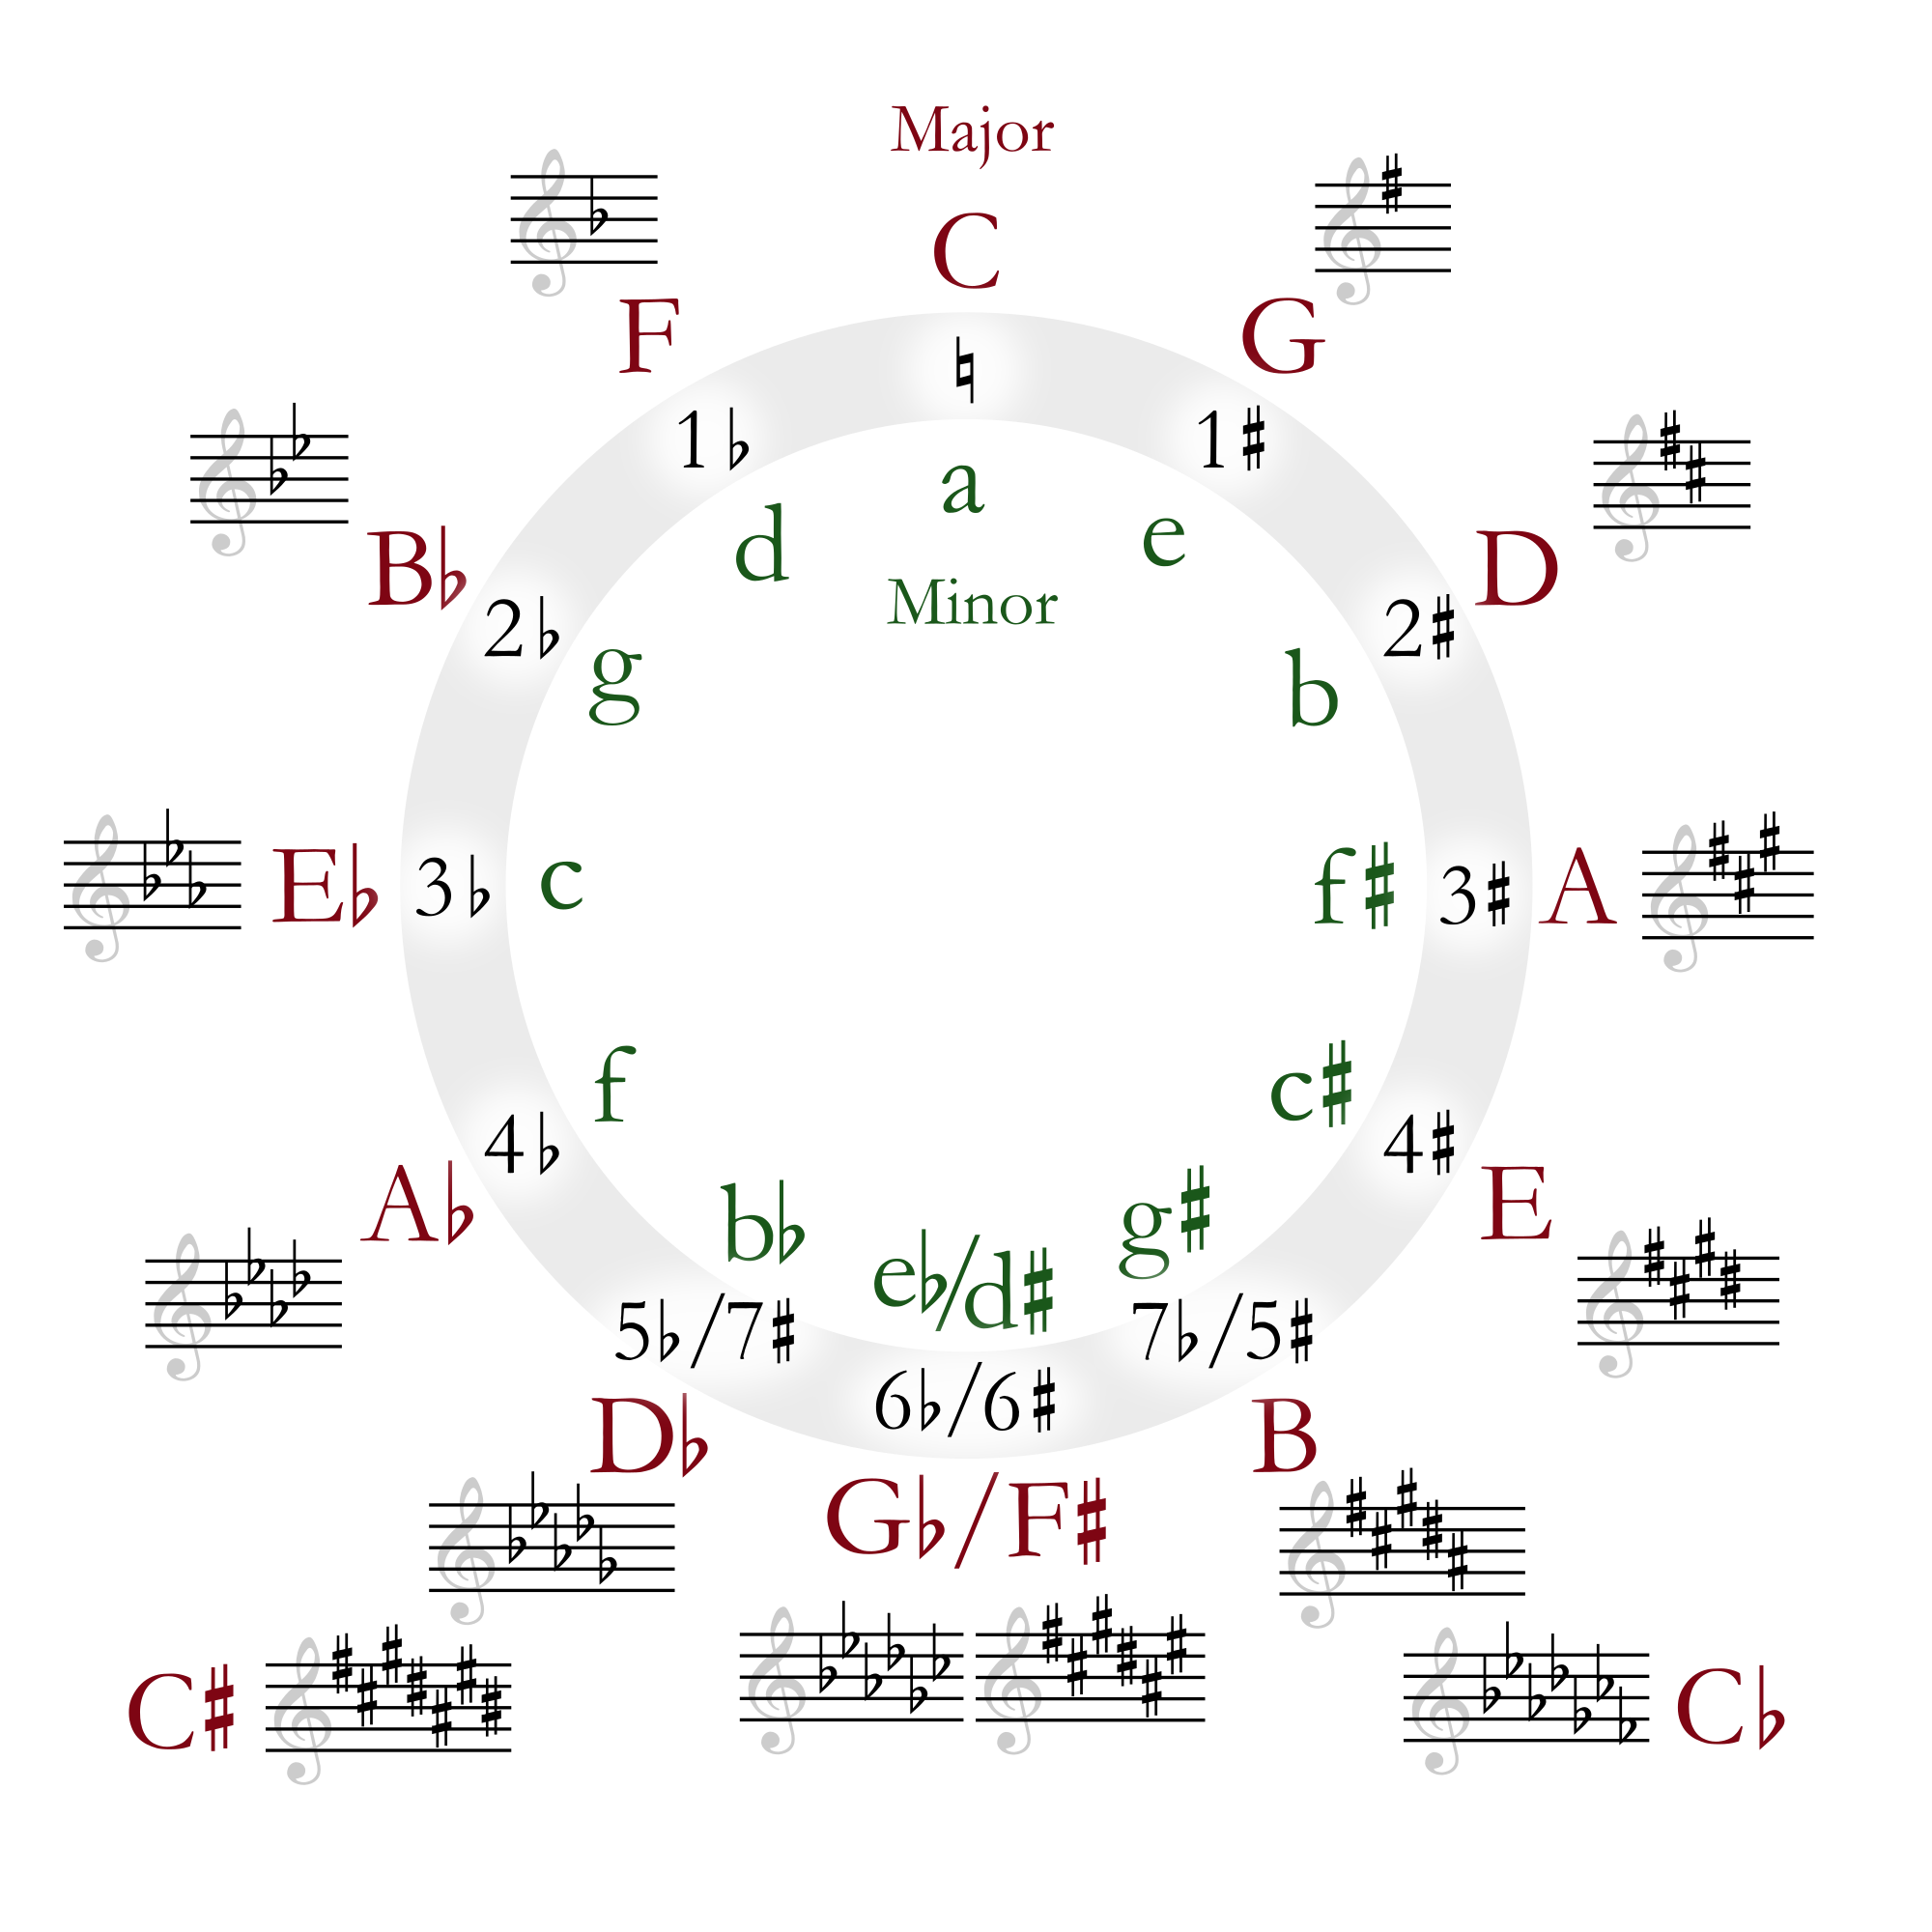
\includegraphics[width=.45\textwidth,keepaspectratio]{aa/circle}
%  \caption{Circolo delle quinte}
%  \label{fig:circle}
% \end{figure}

Non si può far a meno di osservare che la rifrazione negativa di un V\(^{7}\), accordo dominante per eccellenza nella musica occidentale, altro non è che un IVm\(^{6}\), che con il suo colore nostalgico e dolceamaro (e, a questo punto, di "dominante negativo") è certamente uno tra i più diffusi casi in cui si può leggere un'applicazione inconsapevole di quest'idea dell'armonia negativa. Gli esempi di uso di questo accordo sono infiniti; uno dei più iconici è certamente nella coda di piano di \emph{Layla} di Eric Clapton.

\subsubsection{Implicazioni nel nostro brano}
Continuando a parlare del IVm\(^{6}\) osserviamo che la medesima funzione di "dominante negativa (o almeno, così l'abbiamo chiamata in questa trattazione) può essere svolta se muoviamo il basso tre semitoni più in basso, rendendo così l'accordo un IIm\(^{7(\flat5)}\); inoltre, l'aggiunta della settima, nonostante renda l'accordo più interessante e colorato, non è fondamentale nel determinare la funzione dell'accordo, che resta tale anche se l'accordo diventa una semplice triade diminuita II\textsuperscript{dim}; la riflessione positiva di questa triade sarebbe, una nuova triade diminuita costruita sul settimo grado (VII\textsuperscript{dim}), che naturalmente chiama a risolvere verso la tonica.

Ultima assunzione, prima di arrivare al punto: nonostante The Show Must Go On sia, come già detto, un pezzo in SI minore naturale, possiamo analizzarlo considerando la sua relativa maggiore, ossia RE maggiore, dal momento che le note che compongono le due scale sono le medesime.

Qualche riga sopra abbiamo detto che la notazione di A\(\sharp\)\textsuperscript{o}/E è scelta per motivi di \emph{spelling}; dal momento che stavamo pensando quel LA\(\sharp\) come un prestito dalla scala minore armonica di SI, non potevamo certo scriverla come SI\(\flat\). Ovviamente si tratta della stessa nota, per cui non abbiamo alcun problema a pensare a quell'accordo come una triade di E\textsuperscript{dim}, che diventerebbe quindi, rispetto a RE maggiore, il suo secondo grado diminuito, che abbiamo appena dimostrato essere la rifrazione negativa (ma armonicamente equivalente) della triade diminuita costruita sul settimo grado, un DO\(\sharp\)\textsuperscript{dim}. Questo spiega l'origine della componente dominante che sentiamo in quel A\(\sharp\)\textsuperscript{o}/E e conferma, in ultima analisi, di essere una variante di una cadenza d'inganno, ma aggiunge un nuovo livello di mistero, dato dalla sua natura di rifrazione negativa di un accordo già cupo e desolante come un VII\textsuperscript{dim}.

Naturalmente, è estremamente difficile, per non dire impossibile che il compositore del giro avesse in mente tutto questo mentre scriveva, dal momento che il concetto stesso di armonia negativa semplicemente non era ancora stato ripreso; probabilmente ha semplicemente pensato che muovere di un semitono la voce di quel Em suonasse particolarmente efficace, anche se è legittimo pensare che Brian May fosse ben consapevole di star eseguendo quella particolare sostituzione. Tuttavia ho comunque ritenuto questa interpretazione sufficientemente interessante da essere riportata, sia per l'oggettivo fascino che la circonda, sia per dimostrare quanto profonda e quanti livelli possa attraversare l'analisi armonica di un brano di musica leggera.

\subsection{Le altre modulazioni}
A ragion veduta, con le molte parole che abbiamo dedicato alla principale progressione armonica abbiamo quasi esaurito gli elementi importanti da analizzare nel pezzo: come già detto, tutte le sezioni sono costruite su questa progressione, con qualche variazione nel finale per lanciare sezioni specifiche. Tuttavia non si può dimenticare che The Show Must Go On presenta anche non una, ma ben due modulazioni.

\paragraph{Seconda strofa}
Nella seconda strofa del pezzo, infatti, la progressione armonica resta sostanzialmente invariata, ma tutto viene trasposto due semitoni più in alto, in DO\(\sharp\) minore naturale; questo espediente pare sia stato suggerito a May dal produttore \emph{David Richards}. Il cambio di tonalità è introdotto da una misura vuota che segue al ritornello, in cui un arpeggio di chitarra lancia la modulazione. Per tornare a SI minore viene aggiunta una misura alla progressione e viene usato un Em come pivot.

\paragraph{Special}
Questa è l'unica sezione del pezzo che abbandona il giro armonico principale e modula in LA minore naturale. Le prime quattro battute ripetono un giro molto semplice, un \(\flat\)VI - \(\flat\)VII/\(\flat\)VI - Vm\(^{7}\) - Im; nel primo giro viene aggiunto anche un veloce accordo di passaggio, un G\(^{6}\)\textsuperscript{(add\(4\))}. Molto interessante l'uso di quel \(\flat\)VII/\(\flat\)VI, un colore bachiano che all'interno della discografia dei Queen si può ritrovare anche nel ritornello di \emph{Under Pressure}.

\begin{figure}[H]
 \centering
 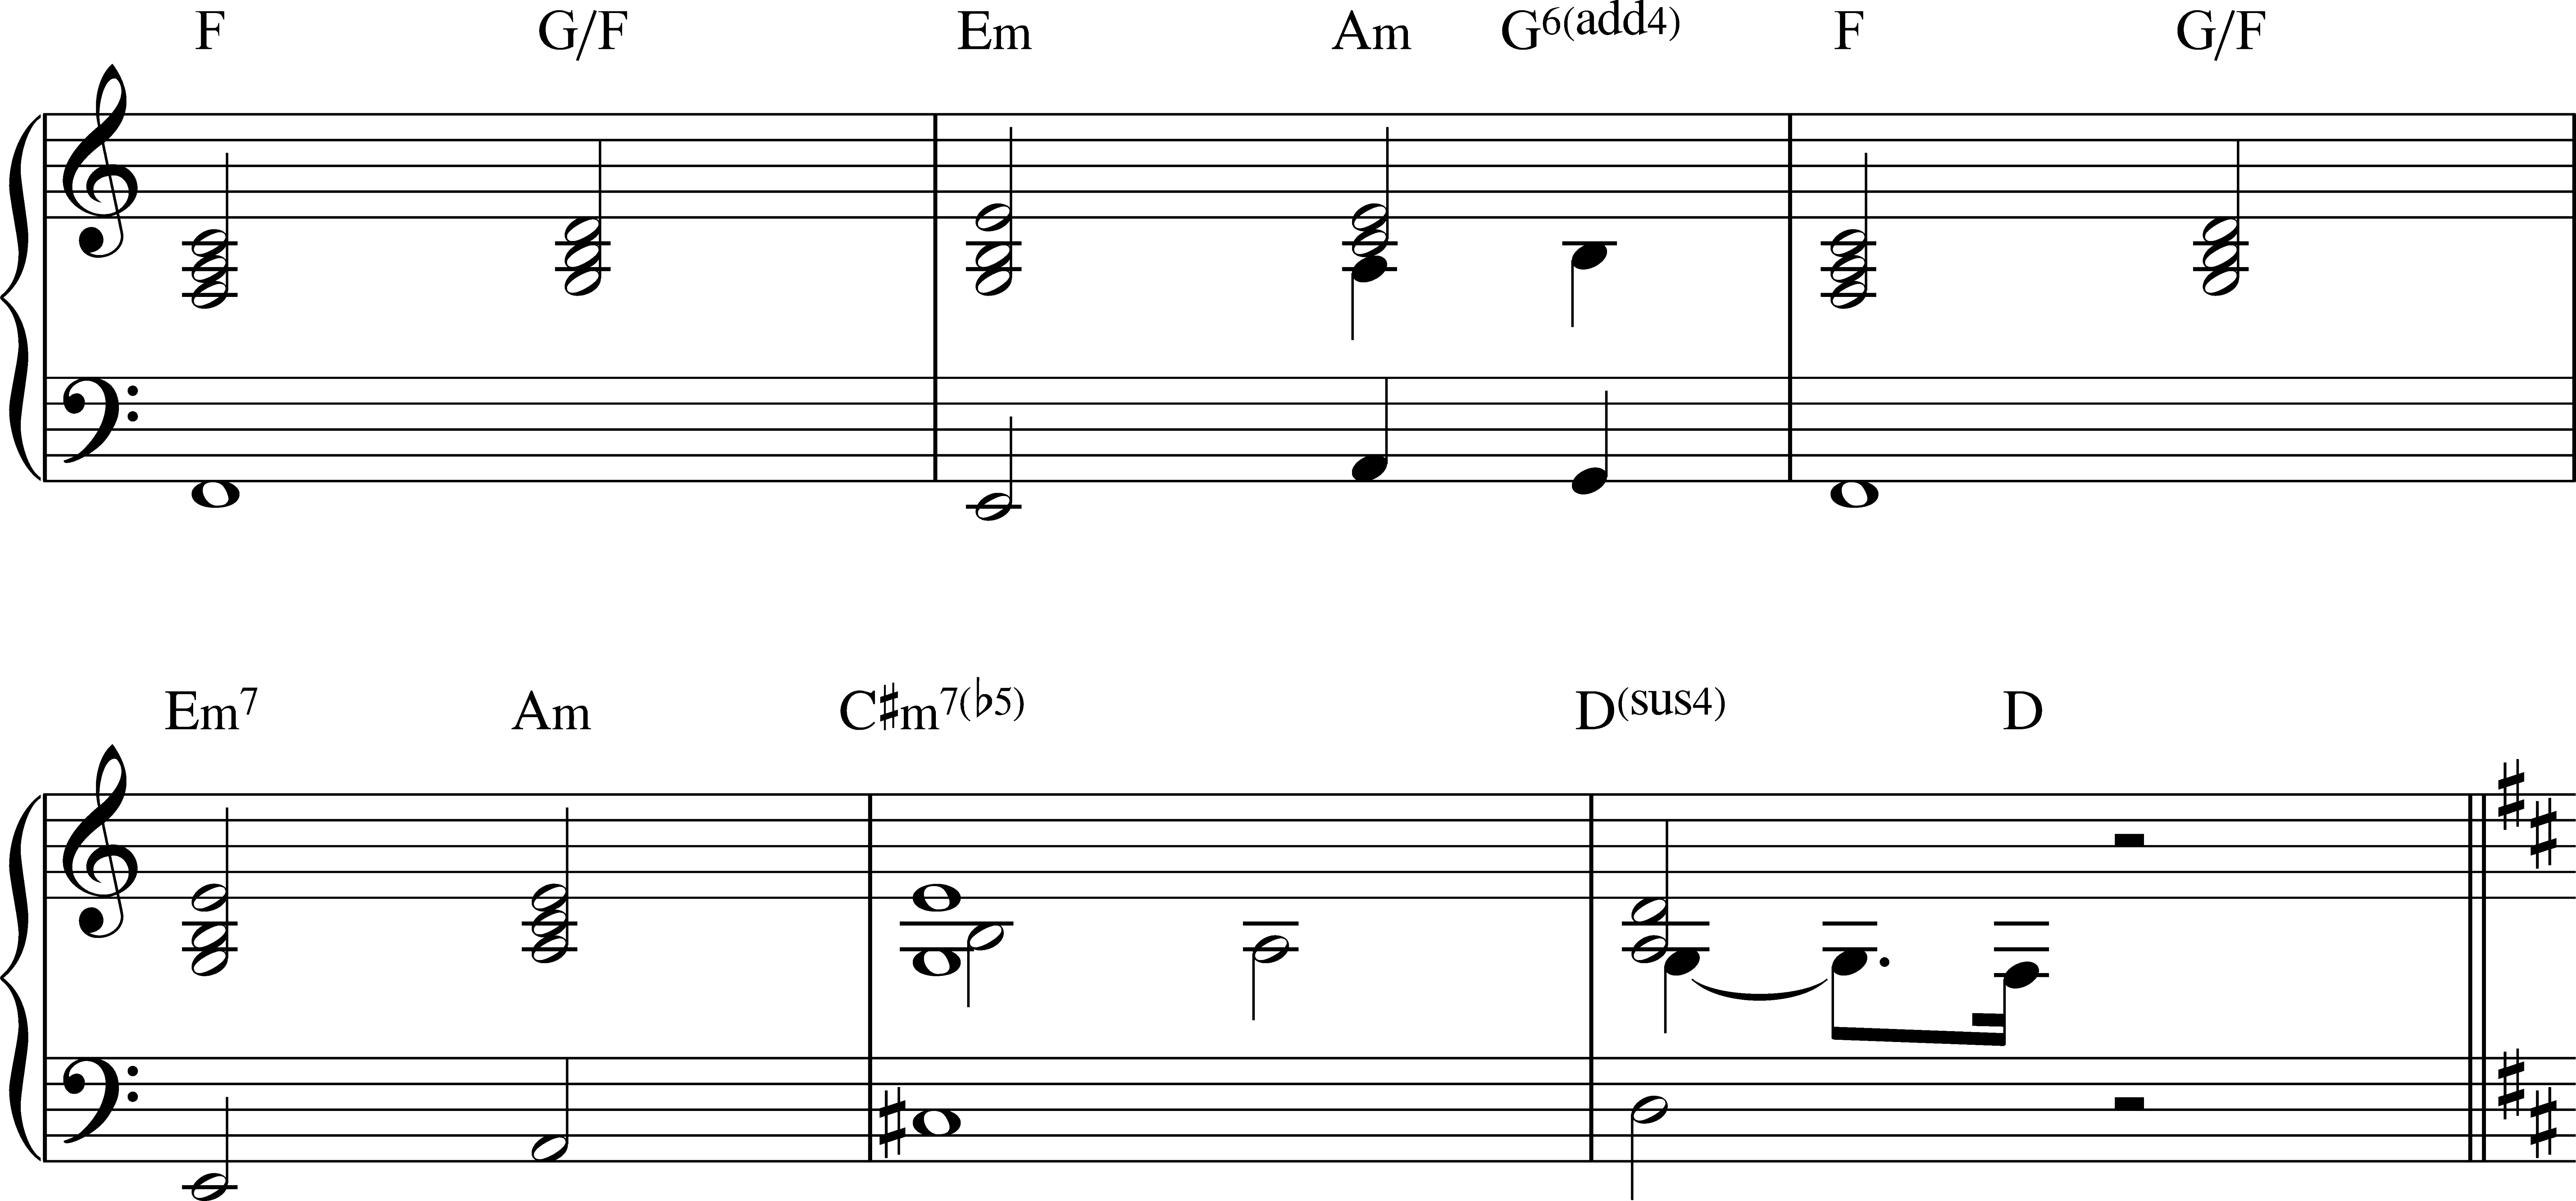
\includegraphics[width=\textwidth,keepaspectratio]{aa/special-chords}
 \caption{Progressione armonica dello special}
 \label{fig:special}
\end{figure}

Come accordo pivot in questo caso viene scelto un C\(\sharp\)m\(^{7(\flat5)}\), che sappiamo essere la quadriade costruita sul secondo grado di SI minore naturale. Nonostante l'accordo ricopra un'intera misura, la voce della settima viene abbassata di un tono dopo due pulsazioni, in modo da rendere più fluido il passaggio ai successivi D\textsuperscript{(sus\(4\))} e D, che riportano il centro tonale verso RE e SI minore.

\section{Considerazioni finali}
Questa è la conclusione del percorso che ci ha portati ad analizzare \emph{The Show Must Go On}, uno dei pezzi più iconici dei \emph{Queen}. Ho pensato che questi fossero un buon candidato sia perché a loro volta sono una tra le formazioni rock più influenti e riconoscibili del loro periodo, sia perché sono stati il gruppo che ha iniziato me alla musica e ha segnato pesantemente una considerevole porzione del mio percorso musicale.

La stesura di questo elaborato mi ha dato l'opportunità di analizzare quali fossero i motivi per cui i Queen sono riusciti a colpirmi in modo così particolare, nei miei \(14\) anni, e se questi potessero in qualche modo destarmi lo stesso interesse anche molti anni dopo. Ho piacevolmente constatato che l'atipicità e la relativa complessità delle composizioni dei Queen, perlomeno rispetto ai canoni della musica pop/rock, riescono a darmi molto da riflettere ancora oggi, nonostante in anni di studio e approfondimento io abbia avuto modo di conoscere moltissimi pattern ed espedienti armonici la cui conoscenza mi fa suonare alcuni pezzi radiofonici quasi banali. Allo stesso modo ho apprezzato la capacità di sintesi di idee e stili che i Queen sono stati capaci di creare.

Ho scelto The Show Must Go On perché mi sembrava un buon compromesso, meno inflazionata ed impegnativa di pezzi come ad esempio Bohemian Rhapsody; ma nonostante questo, ricerca e riflessioni su questo pezzo sono risultate estremamente impegnative e stimolanti, e sono piacevolmente stupito di aver trovato idee ed espedienti interessanti e sono genuinamente felice che la composizione di questo testo mi abbia permesso di sviluppare capacità essenziali come ascolto critico e analisi.

In ultima istanza, spero che anche il lettore abbia potuto trovare qualcosa di interessante in questo testo, e mi auguro che eventuali imprecisioni presenti nell'elaborato non vengano percepite come leggerezza o, ancor peggio, supponenza, ma siano contestualizzate come tentativi di una coscienza musicale ancora in via di formazione di trarre conclusioni e articolare discorsi per cui essa non è ancora sufficientemente preparata.

\newpage

% Initialising backmatter
\appendix

\section{Testo integrale}
\vspace{3cm}
\poemtitle*{The Show Must Go on}
\settowidth{\versewidth}{On and on, does anybody know what we are looking for...}
\begin{verse}[\versewidth]
 Empty spaces - what are we living for \\
 Abandoned places - I guess we know the score \\
 On and on, does anybody know what we are looking for... \\
 Another hero, another mindless crime \\
 Behind the curtain, in the pantomime \\
 Hold the line, does anybody want to take it anymore\\!
 The show must go on \\
 The show must go on \\
 Inside my heart is breaking \\
 My make up may be flaking \\
 But my smile still stays on \\!
 Whatever happens, I'll leave it all to chance \\
 Another heartache, another failed romance \\
 On and on, does anybody know what we are living for... \\
 I guess I'm learning, I must be warmer now \\
 I'll soon ber turning round the corner now \\
 Outside the dawn is breaking \\
 But inside in the dark I'm aching to be free \\!
 The show must go on \\
 The show must go on \\
 Inside my heart is breaking \\
 My make up may be flaking \\
 But my smile still stays on \\!
 My soul is painted like the wings of butterflies \\
 Fairy tales of yesterday will grow but never die \\
 I can fly, my friends \\!
 The show must go on \\
 The show must go on \\
 I'll face it with a grin \\
 I'm never giving in \\
 On, with the show \\!
 I'll top the bill \\
 I'll overkill \\
 I have to find the will to carry on \\
 On with the show \\
 The show must go on
\end{verse}
\attrib{Brian May, 1991}

\section{Innuendo tracklist}

\begin{enumerate}[noitemsep]
 \item \emph{Innuendo} - \(6:31\) (Mercury, Taylor)
 \item \emph{I'm Going Slightly Mad} - \(4:22\) (Mercury)
 \item \emph{Headlong} - \(4:38\) (May)
 \item \emph{I Can't Live With You} - \(4:33\) (May)
 \item \emph{Don't Try So Hard} - \(3:39\) (Mercury)
 \item \emph{Ride the Wild Wind} - \(4:42\) (Taylor)
 \item \emph{All God's People} - \(4:21\) (Mercury, Mike Moran)
 \item \emph{These Are the Days of Our Lives} - \(4:15\) (Taylor)
 \item \emph{Delilah} - \(3:35\) (Mercury)
 \item \emph{The Hitman} - \(4:56\) (Mercury, May, Deacon)
 \item \emph{Bijou} - \(3:36\) (Mercury, May)
 \item \emph{The Show Must Go On} - \(4:35\) (May)
\end{enumerate}

\newpage

\section{Fonti}
In questa sezione vengono presentate le referenze usate per comporre l'elaborato. Lo schema usato è il seguente:

\begin{itemize}
 \item per i libri: [autore dell'opera], \textit{[titolo dell'opera]}, [editore], [informazioni addizionali], [anno];
 \item per le risorse digitali: [autore del contenuto], \textit{[nome del contenuto]}, \texttt{[URL]}.
\end{itemize}

\begin{thebibliography}{99}

 \bibitem{wiki_queen}
 Wikipedia,
 \textit{Queen (band)},
 \texttt{\url{https://en.wikipedia.org/wiki/Queen_(band)}}.

 \bibitem{wiki_smile}
 Wikipedia,
 \textit{Simle (band)},
 \texttt{\url{https://en.wikipedia.org/wiki/Smile_(band)}}.

 \bibitem{wiki_mercury}
 Wikipedia,
 \textit{Freddie Mercury},
 \texttt{\url{https://en.wikipedia.org/wiki/Freddie_Mercury}}.

 \bibitem{wiki_may}
 Wikipedia,
 \textit{Brian May},
 \texttt{\url{https://en.wikipedia.org/wiki/Brian_May}}.

 \bibitem{wiki_taylor}
 Wikipedia,
 \textit{Roger Taylor (Queen Drummer)},
 \texttt{\url{https://en.wikipedia.org/wiki/Roger_Taylor_(Queen_Drummer)}}.

 \bibitem{wiki_deacon}
 Wikipedia,
 \textit{John Deacon},
 \texttt{\url{https://en.wikipedia.org/wiki/John_Deacon}}.

 \bibitem{wiki_innuendo}
 Wikipedia,
 \textit{Innuendo (album)},
 \texttt{\url{https://en.wikipedia.org/wiki/Innuendo_(album)}}.

 \bibitem{wiki_smile}
 Wikipedia,
 \textit{Simle (band)},
 \texttt{\url{https://en.wikipedia.org/wiki/Smile_(band)}}.

 \bibitem{wiki_show}
 Wikipedia,
 \textit{The Show Must Go On (Queen song)},
 \texttt{\url{https://en.wikipedia.org/wiki/The_Show_Must_Go_On_(Queen_song)}}.

 \bibitem{mercury_voice_1}
 NPR Music (non sono riuscito a reperire informazioni sull'autore dell'articolo),
 \textit{Why Freddie Mercury's Voice Was So Great, As Explained By Science},
 \texttt{\url{https://www.npr.org/2016/04/25/475611808/why-freddie-mercurys-voice-was-so-great-as-explained-by-science}}.

 \bibitem{mercury_voice_2}
 Alexander McNamara per ScienceFocus,
 \textit{Why did Freddie Mercury sound so good?},
 \texttt{\url{https://www.sciencefocus.com/the-human-body/why-did-freddie-mercury-sound-so-good/}}.

 \bibitem{innuendo_documentary}
 Estratto di un documentario uscito su VHS e girato nel \(1991\),
 \textit{Queen, Innuendo Electric Press Kit},
 \texttt{\url{https://www.youtube.com/watch?v=VQDZDsEoAyE}}.

 \bibitem{adsr_korg}
 ADSR Music Production Tutorials,
 \textit{Korg M1 - Gear Chat 04},
 \texttt{\url{https://www.youtube.com/watch?v=PK4Id0a_c5g}}.

 \bibitem{html1}
 Tale "Bobby Blues",
 \textit{M1 Description},
 \texttt{\url{http://bobbyblues.recup.ch/korg_m1/m1_description.html}}.

 \bibitem{html2}
 Tale "Bobby Blues",
 \textit{M1 Famous Examples},
 \texttt{\url{http://bobbyblues.recup.ch/korg_m1/m1_examples.html}}.

 \bibitem{lyrics_1}
 Utente anonimo per www.lyricinterpretations.com,
 \textit{Queen: Show Must Go On Meaning},
 \texttt{\url{https://www.lyricinterpretations.com/queen/show-must-go-on}}.

 \bibitem{lyrics_2}
 Adam McDonald,
 \textit{Queen – The Show Must Go On (Lyrics Review and Song Meaning)},
 \texttt{\url{https://justrandomthings.com/2018/11/20/queen-the-show-must-go-on-lyrics-review-and-song-meaning/}}.

 \bibitem{queen_gr_i}
 Richard Gray,
 \textit{Queen - Greatest Hits (Off the record)},
 published by Queen Music Ltd. / EMI music publishing Ltd,
 music transcribed by Barnes Music Engraving Ltd.,
 \(1992\).

 \bibitem{queen_gr_ii}
 Richard Gray,
 \textit{Queen - Greatest Hits II (Off the record)},
 published by Queen Music Ltd. / EMI music publishing Ltd,
 music transcribed by Barnes Music Engraving Ltd.,
 \(1992\).

 \bibitem{voice_yt}
 Mark Ajax,
 \textit{Freddie Mercury VOICE analysis: "The Show Must Go On"},
 \texttt{\url{https://www.youtube.com/watch?v=ic4qxviMP7U&t=258s}}.

 \bibitem{levy}
 Ernst Levy,
 \textit{A Theory of Harmony},
 State University of New York Press,
 \(1985\).

 \bibitem{neely_na}
 Adam Neely,
 \textit{Q+A \#30 - What is negative harmony?},
 \texttt{\url{https://www.youtube.com/watch?v=iHPFAQj0Geg&t=367s}},
 da \(2:32\) a \(7:23\).

 \bibitem{quora_na}
 Curtis Lindsay, utente Quora, in risposta a
 \textit{What is negative Harmony in music?},
 \texttt{\url{https://www.quora.com/What-is-negative-harmony-in-music}}.

 \bibitem{bach}
 Autore anonimo,
 \textit{The Show Must Go On - Songwriting Analysis},
 \texttt{\url{https://www.queensongs.info/song-analysis/songwriting-analyses/modern-era-queen/innuendo/the-show-must-go-on}}.

\end{thebibliography}

\end{document}
